\documentclass[11pt,oneside,openany,report]{jsbook}

\usepackage[a4paper,truedimen,margin=25truemm]{geometry}
\usepackage{cscover}
\usepackage[dvipdfmx]{graphicx}
\usepackage[nobreak]{cite}
\usepackage[a4paper,dvipdfmx,pdfdisplaydoctitle=true,%
    bookmarks=true,bookmarksnumbered=true,bookmarkstype=toc,bookmarksopen=true,%
    pdftitle={グラフ構造によるアルゴリズムの表現を用いたAutoML-Zeroの提案},%
    pdfauthor={三嶋 隆史}%
    ]{hyperref}
\usepackage{pxjahyper}

%追加
\usepackage{amsmath,amssymb}
\usepackage{bbm}
\usepackage{bm}
\usepackage[dvipdfmx]{graphicx}
\usepackage[dvipdfmx]{xcolor}
\usepackage{ascmac}
\usepackage{mathtools}
\usepackage{comment}
\usepackage{subfigure}
\usepackage{algorithm,float}
\usepackage{algorithmic}
\usepackage{setspace}
\usepackage{multirow}
\usepackage{lscape}
\usepackage{fullpage}
\usepackage{ulem}
\usepackage{listings,jvlisting}
\usepackage{longtable}
\usepackage{multicol}
\lstset{
  basicstyle={\ttfamily},
  identifierstyle={\small},
  commentstyle={\smallitshape},
  keywordstyle={\small\bfseries},
  ndkeywordstyle={\small},
  stringstyle={\small\ttfamily},
  frame={tb},
  breaklines=true,
  columns=[l]{fullflexible},
  numbers=left,
  xrightmargin=0zw,
  xleftmargin=3zw,
  numberstyle={\scriptsize},
  stepnumber=1,
  numbersep=1zw,
  lineskip=-0.5ex,
  escapeinside={<@}{@>}
}

\renewcommand{\lstlistingname}{Code.}
\renewcommand{\figurename}{Fig.}
\renewcommand{\tablename}{Table.}
\newcommand{\red}[1]{\textcolor{red}{#1}}
\newcommand{\green}[1]{\textcolor[rgb]{0.1,0.6,0.1}{\textbf{#1}}}
\newcommand{\blue}[1]{\textcolor[rgb]{0.1,0.1,1}{\textbf{#1}}}
\newcommand{\erase}[1]{\textcolor{red}{\sout{\textcolor{black}{\textbf{#1}}}}}
\renewcommand{\bibname}{参考文献}
\renewcommand{\algorithmicrequire}{\textbf{Input:}}
\renewcommand{\algorithmicensure}{\textbf{Output:}}
\newcommand{\TODO}[1]{\textbf{[TODO: #1]}}

\newenvironment{breakablealgorithm}
  {% \begin{breakablealgorithm}
   \begin{center}
     \refstepcounter{algorithm}% New algorithm
     \hrule height.8pt depth0pt \kern2pt% \@fs@pre for \@fs@ruled
     \renewcommand{\caption}[2][\relax]{% Make a new \caption
       {\raggedright\textbf{Algorithm~\thealgorithm} ##2\par}%
       \ifx\relax##1\relax % #1 is \relax
         \addcontentsline{loa}{algorithm}{\protect
umberline{\thealgorithm}##2}%
       \else % #1 is not \relax
         \addcontentsline{loa}{algorithm}{\protect
umberline{\thealgorithm}##1}%
       \fi
       \kern2pt\hrule\kern2pt
     }
  }{% \end{breakablealgorithm}
     \kern2pt\hrule\relax% \@fs@post for \@fs@ruled
   \end{center}
  }

\title{グラフ構造によるアルゴリズムの表現を用いたAutoML-Zeroの提案}
\thesistype{修士論文}
\author{三嶋 隆史}
\studentid{23M31318}
\affiliation{東京科学大学\\情報理工学院\\情報工学系 知能情報コース}
\date{2025年1月}

\supervisorname{指導教員}
\supervisor{小野 功}
\date{\today}


\begin{document}

\frontmatter

\maketitle

\chapter{概要}

本論文では, グラフ構造によるアルゴリズムの表現を導入した AutoML-Zero 手法を提案する. AutoML-Zeroは, 人間からの前提知識をほとんど使わずに, 機械学習タスクを最適に解くことができるアルゴリズムを探索する分野であり, 従来のAutoMLで専門家に依存していた部分を完全に自動化できるという点で重要である. Estebanらが提案したAutoML-Zero手法は, Regularized Evolution (RE)という世代交代モデルを用いた進化計算によって最適な機械学習アルゴリズムを探索する. Estebanらの手法は, 人間による事前知識をほとんど利用していないにも関わらず, 勾配降下法やReLU関数の再発明に成功している. しかし, Estebanらの手法は探索効率の観点で3つの問題があると考えられる. 1つ目は, 探索空間の冗長性の問題である. Estebanらの手法は, 実行結果が同じで変数名や命令の順序のみが異なるアルゴリズムを同一視できない点や機械学習アルゴリズムとして非妥当なアルゴリズムが探索対象となっている点で, 探索空間が冗長となっている. 2つ目は, 良質な構造を子個体に継承できない問題である. Estebanらの手法は, 突然変異で非妥当なアルゴリズムが生成されたり, 元のアルゴリズムが大きく破壊的に変更されたりするため, 良質な構造の継承が難しい. 3つ目は,世代交代において, 集団の多様性が維持しにくいREが使われている問題である. そこで, 本研究では, これらの問題に対処した手法を提案する. 本研究では, グラフ構造を用いてアルゴリズムを表現する手法を導入した上で, 非妥当なアルゴリズム定式化することで探索空間から除外する. また, グラフ構造に基づく突然変異操作を導入し, アルゴリズムの破壊的な変更や非妥当なアルゴリズムへの変更を防止する. さらに, 集団の多様性を維持するために, Minimal Generation Gap (MGG) による世代交代, 集団内の同一個体の排除, および希少度を考慮した生存選択を導入する. 提案手法は, 線形回帰問題において既存手法の1/1000の評価回数で最適解の発見に成功し. 非線形回帰問題では適合度を42\%上昇させることに成功した.

\tableofcontents
\listoffigures
\listoftables

\mainmatter

\chapter{序論}\label{chap:intr}

\section{研究の背景と目的}\label{sec:intr:background}

AutoMLは, 機械学習のモデルを自動で最適化する手法として注目されてきた. AutoML登場以前は, 機械学習のモデルを最適化を人間の手でしていたため, 高度な専門知識と膨大な時間を必要としていた. AutoMLはこの膨大にかかる最適化プロセスをコンピュータに置き換えることを目指してきた分野であり\cite{Fahlman_1989}\cite{Hutter_2011}\cite{Finn_2017}, 今後の機械学習の進歩において非常に重要である. これまでのAutoMLに関する研究の多くは, 計算コストを抑えるために人間のデザインに大きく依存した制約付きの空間を探索している. 例えば, ニューラルネットワークの構造探索では, 事前に専門家が用意した経験則的に性能が高くなる層を構成要素として使うことで, 最適化の対象を構成要素の組合わせやハイパーパラメータに限定したり, 重みの更新方法として常に誤差逆伝搬法を用いることで探索空間を制限している\cite{Zoph_2016}\cite{Real_2019}\cite{Tan_2019}. 他のAutoMLでも同様に, 誤差逆伝搬法の学習ルール, データの増強, 強化学習における好奇心に基づく内部報酬といったアルゴリズムの特定の要素のみを最適化対象とすることで探索空間を限定している\cite{Andrychowicz_2016}\cite{Cubuk_2019}\cite{Alet_2020}.

Estebanらが言及しているように, 探索空間を限定する既存のAutoMLには, 主に2つの問題点が存在する\cite{automl_zero}. 1つ目は, 人間がデザインした探索空間にはバイアスがかかってしまい, 人間がまだ発見していないより良いアルゴリズムを見つけられる可能性が減少してしまう点である. 実際, Elskenらによって, 探索空間の制限は性能に影響を大きく影響を与える観点が無視されることがあることが報告されている\cite{Yang_2019}. 2つ目は探索空間を限定する際は, 極めて慎重に行う必要があり\cite{Zoph_2018}\cite{So_2019}\cite{Negrinho_2019}, 結果的に研究者に負担が掛かってしまう点である. これは, AutoMLの本来の目的である人間の介入を最小限にするという点に反する.

Estebanらは, これらのAutoMLにおける課題を解決するため, 人間からの入力を最小限に抑えた機械学習アルゴリズムの探索手法AutoML-Zeroを提案した\cite{automl_zero}. AutoML-Zeroは, Regularized Evolution (RE) を世代交代モデルとして採用した進化計算により, 与えられた機械学習タスクの集合内の各タスクに対する適合度を最大化する機械学習アルゴリズムを探索する. 機械学習タスクに対するアルゴリズムの適合度は, 学習データを用いて学習した後, 検証データに対する損失の平均を$[0,1]$の範囲に変換した値として定義される. AutoML-Zeroでは, 機械学習アルゴリズムを仮想メモリ上で動作するプログラムとして表現する. プログラムはSetup, Predict, Learnの3つの関数で構成され, 各関数内では高校数学レベルの基本的な演算のみが許可されている. アルゴリズムの改善は, REによる突然変異を通じて行われる. 具体的な突然変異操作として, 命令の追加・削除, 変数アドレスの書き換え, および関数全体のランダムな初期化が実装されている. このように, 人間の事前知識をほとんど使用しない設計にもかかわらず, AutoML-Zeroは勾配降下法やReLU関数の再発明に成功するなど, 注目すべき成果を示している\cite{automl_zero}. また, Estebanらの貢献をベースとして, 様々なAutoML-Zeroの拡張が提案されている. 例えばGuhaらは, 精度と計算コストのトレードオフ構造を考慮した多目的のAutoML-Zero (Moaz) を提案している\cite{multi_objective_automl_zero}. AutoML-Zeroの最適化対象が適合度のみであることに対して, Moazでは計算コストも考慮した多目的の最適化を行っている. また, Haoらによって, AutoML-Zeroの探索手法を利用して損失関数のみを探索する手法も提案されている\cite{auto_loss_zero}.

しかしながら, EstebanらのAutoML-Zeroは人間の事前知識や介入を最小限に抑えつつ機械学習アルゴリズムを自動探索するという画期的な成果を示した一方で, その探索効率には重要な課題が残されている. 例えば, ReLU関数の再発明に成功し, CIFAR-10やMNISTデータセットに対する分類アルゴリズムを発見したSection 4.2の実験では, 膨大な計算リソースが必要とされた. 具体的には, 1秒間あたり10,000モデルの評価が可能なCPUを搭載したマシンを10,000台使用し, 約5日間, 評価回数にして$10^{12}$オーダーの計算を実行している. このような大規模な計算リソースの要求は, 現実的な環境下での応用可能性を制限していると考えられる.

我々は, AutoML-Zeroにおいて探索効率を低下させ得る3つの要因に着目した. 第一に, 探索空間の冗長性が挙げられる. 既存手法では, 変数名や実行順序のみが異なり, 実行結果が同等であるアルゴリズムが別々のアルゴリズムとして扱われ, 探索空間が冗長となっている. また, 機械学習アルゴリズムとして非妥当なアルゴリズムまでもが探索対象に含まれている. 例えば, 予測ラベルが代入されないアルゴリズム, 入力ベクトルが予測に利用されていないアルゴリズム, 逐次更新される学習パラメータが存在しないアルゴリズム, 学習時に正解ラベルを利用していないアルゴリズム, 予測に無関係な変数が存在するアルゴリズムが探索対象となっている. これらの要因により, 既存手法では無意味な評価が多く発生し, 探索効率を低下していると考えられる. 第二に, 突然変異操作に関する2つの問題が挙げられる. 一つは, 非妥当な突然変異が多く発生し, 探索が非効率になる問題である. ここで非妥当な突然変異とは, 親個体が妥当なアルゴリズムであるにも関わらず, 非妥当なアルゴリズムに変化してしまう突然変異を意味する. また既存手法では, 関数全体をランダムに再構成する破壊的な突然変異が高確率で発生する. 故に, 関数中の良質な部分命令列を保存しつつ, 関数を逐次改善することが難しいと考えられる. 第三に, 集団の多様性維持に関する問題が挙げられる. 既存手法で採用されている世代交代モデルREは, 佐藤らの研究が示唆するように, 集団の多様性維持が困難であると考えられる\cite{mgg}. さらに, 集団内における個体の重複や希少度が考慮されていないため, 同一もしくは類似したアルゴリズムが集団内に過度に増加してしまう傾向があると考えられる. これにより, 有望な個体が早期に淘汰され, 局所最適なアルゴリズムに収束する問題が生じる可能性がある.

本研究の目的は, 人間の事前知識や介入を最小限に抑えて機械学習アルゴリズムの探索が可能であるというAutoML-Zeroの利点を保持しつつ, 探索効率を改善した新たな手法を提案することである. 具体的には, 既存手法の問題点に対処した手法を提案し, 評価回数を揃えて探索を行った時に, 既存手法よりも高い適合度を持つアルゴリズムの発見できることを確かめる. 提案手法では, グラフ構造を用いてアルゴリズムを表現する手法(アルゴリズムグラフ)を導入する. アルゴリズムグラフはプログラムの本質的な依存関係のみを抽出するFerrantらが提案した中間表現形式PDGの考え方を参考にして導入した\cite{vag}. グラフ構造を用いることで, 変数名や実行順が異なるだけで実行結果は同じアルゴリズムを同一視することが可能となる. その上で, アルゴリズムグラフに対して, 機械学習アルゴリズムとして満たすべき条件(妥当なアルゴリズムの条件)を明確に規定し, 条件を満たさないアルゴリズムを探索空間から除外する. これにより, 探索空間の冗長性の削減を目指す. また, アルゴリズムグラフに対する突然変異を導入することで, 非妥当な突然変異が起こらないように設計する. 加えて, 部分グラフの再構成を用いた新たな突然変異により, アルゴリズムの関数内の部分命令列を局所的に変更することを実現する. 突然変異の工夫により, 近傍探索性能が向上し, より効率的な探索ができると期待される. さらに, 集団の多様性を維持するために, Minimal Generation Gap (MGG) \cite{mgg}による世代交代モデル, 集団内の同一個体の重複排除, および希少度に基づく生存選択を導入する. これにより, 有望な個体が早期に淘汰され, 局所最適なアルゴリズムに収束する問題を防ぐことが期待できる.

\section{本論文の貢献}\label{sec:intr:contribution}

本研究の主要な貢献は以下の4点である.

\begin{itemize}
  \item グラフ構造によるアルゴリズム表現の提案: 機械学習アルゴリズムをグラフ構造で表現し, 満たすべき条件を明確に規定した. これにより, 条件を満たさないアルゴリズムを探索空間から排除し, 探索空間を99.9\%以上削減することに成功した. また, アルゴリズムをグラフ構造で表現したことで, 変数名によるアルゴリズムの冗長性の排除をすることができた.
  \item グラフ構造に基づく突然変異操作の提案: グラフ構造を活用した突然変異により, 既存手法で99.6\%以上発生していた非妥当な突然変異を完全に発生しないようにすることができた. さらに, 部分グラフに対する突然変異を導入することで, 特定の変数計算に必要な部分命令列のみを変更可能な突然変異を実現した.
  \item 集団の多様性維持のための手法の提案: Minimal Generation Gap (MGG) による世代交代モデル, 集団内の同一個体の排除, および希少度を考慮した生存選択を導入した. これらの改善により, 集団の多様性が維持され, 早期収束が抑制された結果, アフィン回帰問題において最適解を発見するまでにかかる評価回数を1/3にすることができた.
  \item 提案手法の有効性の検証: ローカルPCという限られた計算リソース環境において, 主要な回帰問題と分類問題を用いた比較実験を実施した. その結果, 非線形回帰問題において同一評価回数内で発見されるアルゴリズムの適合度が42\%以上向上することを確認した. また, 線形回帰問題の最適解を発見するまでの評価回数を比較する実験では, 提案手法は既存手法の1/1000回未満の評価回数で最適解を発見できることがわかった.
\end{itemize}

\section{本論文の構成}\label{sec:intr:structure}
本論文では, 第\ref{chap:intr}章で研究の背景と目的および貢献, 第\ref{chap:problem}章でAutoML-Zeroの問題設定とEstebanらが提案した既存手法の説明と問題点, 第\ref{chap:proposed}章で既存手法の問題点に対処した提案手法の詳細な説明, 第\ref{chap:exp}章で提案手法の有効性を検証するための実験, 第\ref{chap:consideration}章で実験結果の考察や提案手法の各工夫の有効性の検証,  第\ref{chap:conclusion}章で本研究のまとめと今後の課題について述べる.

\chapter{問題の所在}\label{chap:problem}

\section{はじめに} \label{sec:problem:introduction}
本章では, 第\ref{sec:problem:definition}節で我々が研究対象とするAutoML-Zeroの問題設定の定義を説明した上で, 第\ref{sec:problem:re_automl_zero}節でAutoML-Zeroの既存手法であるRE-AutoML-Zeroについて説明する. その後, 第\ref{sec:problem:existing_problem}節で, 探索空間の冗長性に関する問題, 良質な構造を子個体に継承できない問題, 集団の多様性時に関する問題について述べる.

\section{問題の定義} \label{sec:problem:definition}

本研究で対象とするAutoML-Zeroは, 与えられた機械学習タスク集合$\mathcal{T}$内の各機械学習タスクに対して, 最も高い適合度を達成可能なアルゴリズム$a^\ast \in \mathcal{A}$を, $\mathcal{T}$の代表的な部分集合$\mathcal{T}_\mathrm{search} \subset \mathcal{T}$から探索する問題である. ここで, $\mathcal{A}$はアルゴリズム全体の集合である. 以下, 第\ref{subsec:problem:definition:tasksets}節でタスク集合, 第\ref{subsec:problem:definition:fitness}節で適合度, 第\ref{subsec:problem:definition:optimum}節において最適なアルゴリズムの詳細な説明を行う.

\subsection{タスク集合}\label{subsec:problem:definition:tasksets}

タスク集合$\mathcal{T}$は, 複数の機械学習タスクによって構成される. 各機械学習タスク$T \in \mathcal{T}$は, 入力ベクトル$\bm{x}_j$と正解ラベル$y_j$の順序対の集合であり, 以下のように定義される.

$$
  T = \left\{\left(\bm{x}_j, y_j \right) \ |\ \bm{x}_j \in \mathbb{R}^{d},\ y_j \in \mathbb{R},\ j \in \mathbb{N},\ 1 \le j \le N \right\}
$$

\noindent
ここで, $N$および$d$はそれぞれタスクごとに定まるデータの個数とタスクの次元である. また, タスク$T$には学習用データ$D_\mathrm{train} \subset T$および検証用データ$D_\mathrm{valid} \subset T$が定められており, $D_\mathrm{train} \cup D_\mathrm{valid} = T $, $D_\mathrm{train} \cap D_\mathrm{valid} = \emptyset$を満たす.

\subsection{適合度} \label{subsec:problem:definition:fitness}

アルゴリズム$a$のタスク$T$に対する適合度$F(a, T)$は, 学習データ$D_\mathrm{train}$をアルゴリズム$a$で学習させた上で, 検証データ$D_\mathrm{valid}$に対する損失を$[0,1]$に変換することで計算される. 適合度は, 1に近いほどタスク$T$に適合している, 言い換えれば$T$の検証データに対する損失が小さいことを意味する. 損失や損失を$[0,1]$に変換する関数はユーザによって与えられる. 例えば, 線型回帰のタスクであれば, $D_\mathrm{valid}$に対する予測ラベルと正解ラベルの平均二乗誤差$l$が損失として利用され, 適合度は$1-\frac{2}{\pi} \arctan\left(\sqrt{l}\right)$を用いて, $[0,1]$の区間に変換することで算出される.

\subsection{最適なアルゴリズム}\label{subsec:problem:definition:optimum}

本研究における最適なアルゴリズム$a^\ast \in \mathcal{A}$は, 以下のように定式化される.
\begin{equation}
\label{eq:optimum}
a^\ast =  \arg \max_{a \in \mathcal{A}} \frac{1}{|\mathcal{T}_\mathrm{eval}|} \sum_{T \in \mathcal{T}_\mathrm{eval}} F(a, T)
\end{equation}

\noindent
一般に, $\mathcal{T}$は無限集合であり, $\mathcal{T}$の全タスクに対する適合度の計算は困難である. そのため, $\mathcal{T}$の有限部分集合$\mathcal{T}_\mathrm{eval}$内のタスクに対する適合度の平均を最大化するアルゴリズムを最適なアルゴリズムと定義する. ここで, $\mathcal{T}_\mathrm{eval}$に含まれるタスクは$\mathcal{T}_\mathrm{search}$と同様にタスクの種類に偏りが生じないよう構成する必要がある. また, $\mathcal{T}_\mathrm{search}$への過適合を防ぐため, $\mathcal{T}_\mathrm{search}$と$\mathcal{T}_\mathrm{eval}$は互いに独立に構成する.

最適なアルゴリズムについて具体例を挙げて説明する. $\mathcal{T}$が線形回帰タスク全体$\mathcal{T}_\mathrm{LinReg}$である場合, $\mathcal{T}_\mathrm{LinReg}$内の全タスクに対して誤差0で回帰可能な線型回帰アルゴリズム$a_\mathrm{LinReg} \in \mathcal{A}$が最適なアルゴリズムとなる. 一方, $\mathcal{T}$が一般の回帰問題全体の集合$\mathcal{T}_\mathrm{Reg}$である場合, $\mathcal{T}_\mathrm{Reg}$には線型回帰タスクに加えて非線形回帰タスクも含まれる. このとき, 線型回帰アルゴリズム$a_\mathrm{LinReg}$では非線形回帰問題に対して十分な精度を得られないため, 最適なアルゴリズムとはならない. したがって, 本問題設定では, タスク集合として$\mathcal{T}_\mathrm{LinReg}$が与えられた場合は線型回帰アルゴリズム$a_\mathrm{LinReg}\in \mathcal{A}$が, $\mathcal{T}_\mathrm{Reg}$が与えられた場合は非線形回帰タスクにも対応可能なアルゴリズム$a_\mathrm{Reg}\in \mathcal{A}$が得られることが求められる.

\section{既存手法 RE-AutoML-Zero}\label{sec:problem:re_automl_zero}

本節では, Estebanらが提案したAutoML-Zero手法について述べる. Estebanらが提案した手法は, Regularized Evolution (RE)を使ったAutoML-Zero手法であるため, 以降ではRE-AutoML-Zeroと呼ぶ. 以下, 第\ref{subsec:problem:existing_method:algorithm_exp}項ではRE-AutoML-Zeroにおけるアルゴリズムの表現方法, 第\ref{subsec:problem:existing_method:algorithm_eval}項ではRE-AutoML-Zeroにおけるアルゴリズムの評価方法, 第\ref{subsec:problem:existing_method:re}項ではREによる世代交代, 第\ref{subsec:problem:existing_method:mutation}項では突然変異による個体生成について述べる.

\subsection{アルゴリズムの表現方法}\label{subsec:problem:existing_method:algorithm_exp}

RE-AutoML-Zeroにおいて機械学習アルゴリズムは, 小さな仮想メモリで動作するプログラムとして表される. 仮想メモリには, スカラー, $d$次元ベクトル, $d \times d$次元行列を複数個格納できる.ここで, $d $はタスク集合$\mathcal{T}_\mathrm{search}$に含まれるタスク$T$の入力ベクトルの次元である. 以降, スカラーを格納する変数を$s0,s1,\cdots$, ベクトルを格納する変数を$v0,v1,\cdots$, 行列を格納する変数を$m0,m1,\cdots$と表す. $s0$, $s1$, $v0$は, それぞれ正解ラベル, アルゴリズムによる予測ラベル, 入力ベクトルを格納する先として使われる特別な変数である. その他の変数は学習対象のパラメータを格納したり, 計算結果を一時的に保存する用途で用いられる. 変数の個数の上限はスカラー, ベクトル, 行列それぞれに対してユーザが指定する必要がある.

アルゴリズムは, Code.\ref{code:affine_algorithm}に示したように, Setup, Predict, Learnの3つの関数で表現される. 各関数はTable.\ref{table:instructions}に示した64個の命令の列で構成される. 命令は, 人間のバイアスを与えすぎないようにするため, 高校数学で学ぶ程度の演算のみを使用し, 機械学習のアルゴリズムの概念や行列の分解等の演算は含まれていない. また, 命令に与える引数は, 基本的には仮想メモリに格納されているスカラー$s1,s2,\cdots$, ベクトル$v1,v2,\cdots$, 行列$m1,m2,\cdots$のいずれかである. 一部例外として, 正規分布による乱数生成の命令等では, $\mu$, $\sigma$等の定数が入力されることもある.

\begin{lstlisting}[caption=アフィン回帰と解釈可能なアルゴリズム,label=code:affine_algorithm]
  def Setup():
    s3 = 0.01 // 学習率の設定

  def Predict():
    s2 = dot(v6, v0) // 重みと入力ベクトルの内積を計算
    s1 = s7 + s2 // 切片を加算

  def Learn():
    s4 = s0 - s1 // 予測ラベルと正解ラベルの誤差を計算
    s6 = s3 * s4 // 学習率の適用
    v3 = s6 * v0 // 傾きの更新するための差分を計算
    v6 = v6 + v3 // 傾きを更新
    s7 = s7 + s6 // 切片を更新
\end{lstlisting}



\subsection{アルゴリズムの評価方法}\label{subsec:problem:existing_method:algorithm_eval}

既存手法のアルゴリズムの探索では, 以下の式で定義されるタスク集合 $\mathcal{T}_\mathrm{search}$ に対する適合度 $F(a, \mathcal{T}_\mathrm{search})$ を評価指標として用いる.
\[
F(a, \mathcal{T}_\mathrm{search}) = \frac{1}{\left|\mathcal{T}_\mathrm{search}\right|} \sum_{T \in \mathcal{T}_\mathrm{search}} F(a, T)
\]
この適合度 $F(a, \mathcal{T}_\mathrm{search})$ を最大化するアルゴリズムは, $\mathcal{T}_\mathrm{eval}$のタスクに対しても高い適合度を示すことが期待される.

タスク集合内の1つのタスク$T$に対するアルゴリズムの評価は, Algorithm \ref{algorithm:algorithm_evaluation}に示した流れで行われる. Algorithm \ref{algorithm:algorithm_evaluation}の入力は評価対象のアルゴリズム$a \in \mathcal{A}$, タスク$T \in \mathcal{T}_\mathrm{search}$の学習用データ$D_\mathrm{train}$および検証用データ$D_\mathrm{valid}$であり, 出力は評価対象のアルゴリズムのタスク$T$に対する適合度である.

\begin{breakablealgorithm}
  \caption{タスク$T$に対するアルゴリズムの評価方法}
  \label{algorithm:algorithm_evaluation}
  \begin{algorithmic}[1]
    \REQUIRE 評価対象のアルゴリズム$a=(\mathrm{Setup}, \mathrm{Predict}, \mathrm{Learn})$, タスク$T = D_\mathrm{train} \cup D_\mathrm{valid}$
    \ENSURE タスク$T$に対するアルゴリズムの適合度 $F(a, T)$
    \STATE initialize\_memory()
    \STATE Setup()
    \FOR{$ e = 0, 1, \cdots, N_\mathrm{epochs} $}
    \FORALL{$ (\bm{x}_j, y_j) \in  D_\mathrm{train}$}
    \STATE $v0 \leftarrow \bm{x}_j$
    \STATE Predict()
    \STATE $s1 \leftarrow \mathrm{Normalize}(s1)$
    \STATE $s0 \leftarrow y_j$
    \STATE Learn()
    \ENDFOR
    \ENDFOR
    \STATE $l_\mathrm{sum} = 0.0$
    \FORALL{$ (\bm{x}_j, y_j) \in  D_\mathrm{valid}$}
    \STATE $v0 \leftarrow \bm{x}_j$
    \STATE Predict()
    \STATE $s1 \leftarrow \mathrm{Normalize}(s1)$
    \STATE $l_\mathrm{sum} \leftarrow l_\mathrm{sum} + \mathrm{Loss}(y, s1)$
    \ENDFOR
    \STATE $ l_\mathrm{mean} \leftarrow l_\mathrm{sum} / \left|D_\mathrm{valid}\right|$
    \STATE $ \mathrm{fitness} = \mathrm{Rescale}(l_\mathrm{mean})$
    \RETURN $ \mathrm{fitness} $
  \end{algorithmic}
\end{breakablealgorithm}

Algorithm \ref{algorithm:algorithm_evaluation}の各行の詳細な説明を以下に示す.

\begin{description}
  \item[1行目] 仮想メモリをすべて0で初期化する.
  \item[2行目] Setup関数を実行する.
  \item[3-11行目] 学習用のループを実行する. $N_\mathrm{epochs}$はエポック数であり, 学習用データを使う回数を表す.
    \begin{description}
      \item[4-10行目] $e$番目のエポックに対応する学習を行う. エポックごと$(\bm{x}_j, y_j) \in D_\mathrm{train}$を取り出す順番は異なる.
        \begin{description}
          \item[5行目] $v0$に入力ベクトル$\bm{x}_j$を代入する.
          \item[6行目] Predict関数の実行を行う. 正解ラベル$y_j$は事前に代入されていないので使うことが出来ない. また, Predict関数実行後は, $s1$に予測結果が含まれているものとして扱う.
          \item[7行目] $s1$に格納されている予測結果をNormalize関数を用いて正規化する. Normalize関数は, 回帰タスクの場合には恒等関数, 二値分類タスクの場合にはsigmoid関数などが使われる.
          \item[8行目] 正解ラベルを$s0$に代入する.
          \item[9行目] Learn関数を実行する.
        \end{description}
    \end{description}
  \item[12行目] 検証用データにおける損失の合計を計算するための変数$l_\mathrm{sum}$を初期化する.
  \item[13-18行目] 検証用データ$D_\mathrm{valid}$を用いて検証用ループを実行する.
    \begin{description}
      \item[14行目] 学習用ループと同様に$v0$に入力ベクトル$\bm{x}_j$を代入する.
      \item[15行目] 学習用ループと同様にPredict関数の実行を行う.
      \item[16行目] 学習用ループと同様に予測結果を正規化する.
      \item[17行目] 学習用ループとは異なり, Learn関数の実行はせず予測結果の損失をLoss関数を使って計算する. Loss関数は, 回帰タスクの場合には二乗誤差を返す関数, 二値分類タスクの場合にはの場合には予測ラベルと正解ラベルが一致しているときに1, それ以外のときは0を返す関数である.
    \end{description}
  \item[19行目] 損失の平均値$l_\mathrm{mean}$を計算する.
  \item[20行目] 損失をRescale関数を用いて適合度に変換する. Rescale関数は, 回帰タスクの場合は$\mathrm{Rescale}(l) = 1 - \frac{2}{\pi} \arctan{\sqrt{l}} $, 二値分類タスクの場合は$\mathrm{Rescale}(l) = 1 - l$などが用いられる.
  \item[21行目] 適合度を返却する.
\end{description}

\noindent
1行目で行ったメモリの初期化以降, 特別な変数$s0$, $s1$, $v0$以外の変数への代入は, Setup, Predict, Learnの中以外で行われることがない. そのため, 評価対象のアルゴリズムの各関数Setup, Predict, Learnでは, $s0$, $s1$, $v0$以外の変数に学習対象のパラメータを格納することで, 初期化時から検証時まで当該パラメータの値を引き継ぐことができる.

\subsection{REによる世代交代}\label{subsec:problem:existing_method:re}

\begin{figure}[tbp]
  \centering
  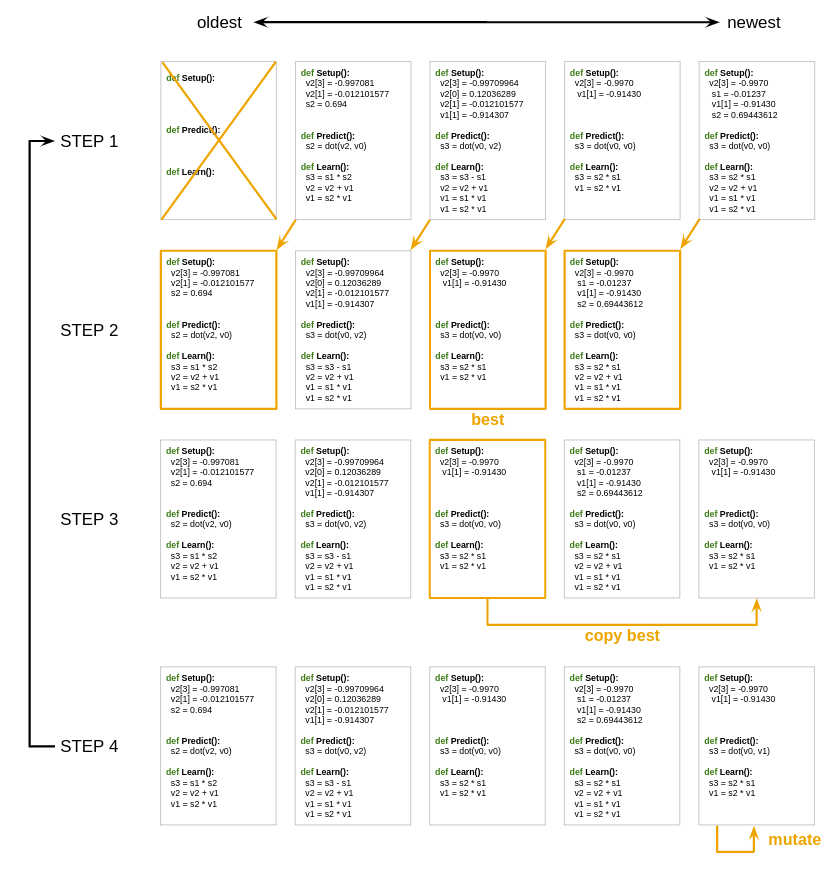
\includegraphics[width=14cm]{problem/existing_method/regularized_evolution.png}
  \caption{RE-AutoML-Zero\cite{automl_zero}の世代交代モデル. STEP1からSTEP4を繰り返すことで最適なアルゴリズムの発見を目指す. STEP1で最も古い個体を削除した後に, STEP2でトーナメント選択を行う. その後, STEP3でトーナメント選択によって選ばれた個体をコピーし, STEP4で一定確率$p_\mathrm{mutate}$で突然変異を行う. }
  \label{fig:regularized_evolution}
\end{figure}


Estebanらが提案したRE-AutoML-Zeroでは, $N_\mathrm{pop}$個のアルゴリズムをランダムに初期集団として生成した後に, Fig.\ref{fig:regularized_evolution}のSTEP1からSTEP4に示したRegularized Evolution (RE) を繰り返し行うことで, 最適なアルゴリズムの探索を行う. REでは, STEP1で最も古い個体を削除した後に, STEP2でトーナメント選択, すなわち$K( < N_\mathrm{pop})$個の個体を非復元抽出した上で最も適合度の高い個体を選択を行う. その後, STEP3でトーナメント選択によって選ばれた個体をコピーし, STEP4で一定確率$p_\mathrm{mutate}$で突然変異を行う. 集団サイズ$N_\mathrm{pop}$, トーナメントサイズ$K$, 突然変異確率$p_\mathrm{mutate}$はユーザパラメータである.

RE-AutoML-Zeroの詳細なアルゴリズムをAlgorithm \ref{algorithm:re_automl_zero}に示す. Algorithm \ref{algorithm:re_automl_zero}の入力はタスク集合$\mathcal{T}_\mathrm{search}$, 集団サイズ$N_\mathrm{pop}$, トーナメントサイズ$K$, 突然変異確率$p_\mathrm{mutate}$, 最大評価回数$ N_\mathrm{eval}$である. また, 出力は探索結果のアルゴリズムである.

\begin{breakablealgorithm}
  \caption{Regularized Evolution (RE) のアルゴリズム}
  \label{algorithm:re_automl_zero}
  \begin{algorithmic}[1]
    \REQUIRE タスク集合$\mathcal{T}_\mathrm{search}$, 集団サイズ$N_\mathrm{pop}$, トーナメントサイズ$K$, 突然変異確率$p_\mathrm{mutate}$, 最大評価回数$ N_\mathrm{eval}$
    \ENSURE 発見されたアルゴリズム
    \STATE $\mathrm{eval\_num} \leftarrow 0 $
    \STATE $P \leftarrow \emptyset $
    \FOR{$ i = 1 $ to $ N_\mathrm{pop}$}
    \STATE $\mathrm{algorithm} \leftarrow  \mathrm{generate\_algorithm}()$
    \STATE $\mathrm{fitness} \leftarrow  F(a, \mathcal{T_\mathrm{search}})$
    \STATE $\mathrm{eval\_num} \leftarrow \mathrm{eval\_num} + 1 $
    \STATE $\mathrm{individual} \leftarrow  (\mathrm{algorithm}, \mathrm{fitness}) $
    \STATE $P \leftarrow P \cup \{ \mathrm{individual} \} $
    \ENDFOR
    \WHILE{$\mathrm{eval\_num} < N_\mathrm{eval}$}
    \STATE $\mathrm{oldest} = \mathrm{get\_oldest}(P)$
    \STATE $ P \leftarrow P \setminus \{ \mathrm{oldest} \} $
    \STATE $(\mathrm{base\_algorithm}, \mathrm{fitness}) \leftarrow \mathrm{tournament\_select}(P, K)$
    \STATE $\mathrm{algorithm} \leftarrow \mathrm{copy}(\mathrm{base\_algorithm})$
    \IF{   $\mathrm{rand}(0, 1) < p_\mathrm{mutate}$}
    \STATE $\mathrm{algorithm} \leftarrow \mathrm{mutate}(\mathrm{algorithm})$
    \STATE $\mathrm{fitness} \leftarrow  F(a, \mathcal{T_\mathrm{search}})$
    \STATE $\mathrm{eval\_num} \leftarrow \mathrm{eval\_num} + 1 $
    \ENDIF
    \STATE $\mathrm{individual} \leftarrow  (\mathrm{algorithm}, \mathrm{fitness}) $
    \STATE $P \leftarrow P \cup \{ \mathrm{individual} \} $
    \ENDWHILE
    \STATE $(\mathrm{best\_algorithm}, \mathrm{best\_fitness}) \leftarrow \mathrm{get\_best\_fitness}(P)  $
    \RETURN $\mathrm{best\_algorithm}$
  \end{algorithmic}
\end{breakablealgorithm}

Algorithm \ref{algorithm:re_automl_zero}の各行の説明を以下に示す.

\begin{description}
  \item[1行目] 評価回数のカウンターを初期化する.
  \item[2行目] 集団$P$を初期化する.
  \item[3-9行目] 集団$P$に$N_\mathrm{pop}$個のアルゴリズムをランダムに生成し, 適合度を計算する.
  \begin{description}
    \item[4行目] アルゴリズムをランダムに生成する関数$\mathrm{generate\_algorithm}()$を実行する.
    \item[5行目] タスク集合$\mathcal{T_\mathrm{search}}$に対するアルゴリズムの適合度を計算する.
    \item[6行目] 評価回数をインクリメントする.
    \item[7行目] アルゴリズムと適合度のペアである個体を作成する.
    \item[8行目] 集団$P$に個体を追加する.
  \end{description}
  \item[10-22行目] 評価回数が上限を超えるまでREによる世代交代を繰り返す.
  \begin{description}
    \item[11行目] 集団$P$から最も古いアルゴリズム(個体)を取り出す関数$\mathrm{get\_oldest}(P)$を実行する.
    \item[12行目] 集団$P$から最も古いアルゴリズムを消去する.
    \item[13行目] 集団$P$からトーナメントサイズ$K$でトーナメント選択する関数$\mathrm{tournament\_select}(P, K)$を実行する.
    \item[14行目] トーナメント選択されたアルゴリズムをコピーする.
    \item[15-19行目] 一定確率$p_\mathrm{mutate}$で突然変異を行う.
    \begin{description}
      \item[16行目] アルゴリズムを突然変異させる関数$\mathrm{mutate}(\mathrm{algorithm})$を実行する.
      \item[17行目] タスク集合$\mathcal{T_\mathrm{search}}$に対するアルゴリズムの適合度を計算する.
      \item[18行目] 評価回数をインクリメントする.
    \end{description}
    \item[20行目] アルゴリズムと適合度のペアである個体を作成する.
    \item[21行目] 集団$P$に個体を追加する.
  \end{description}
  \item[23行目] 集団$P$から最も適合度の高いアルゴリズムを取得する.
  \item[24行目] 最も適合度の高いアルゴリズムを返却する.
\end{description}

\subsection{突然変異による子個体生成}\label{subsec:problem:existing_method:mutation}

\begin{figure}
  \centering
  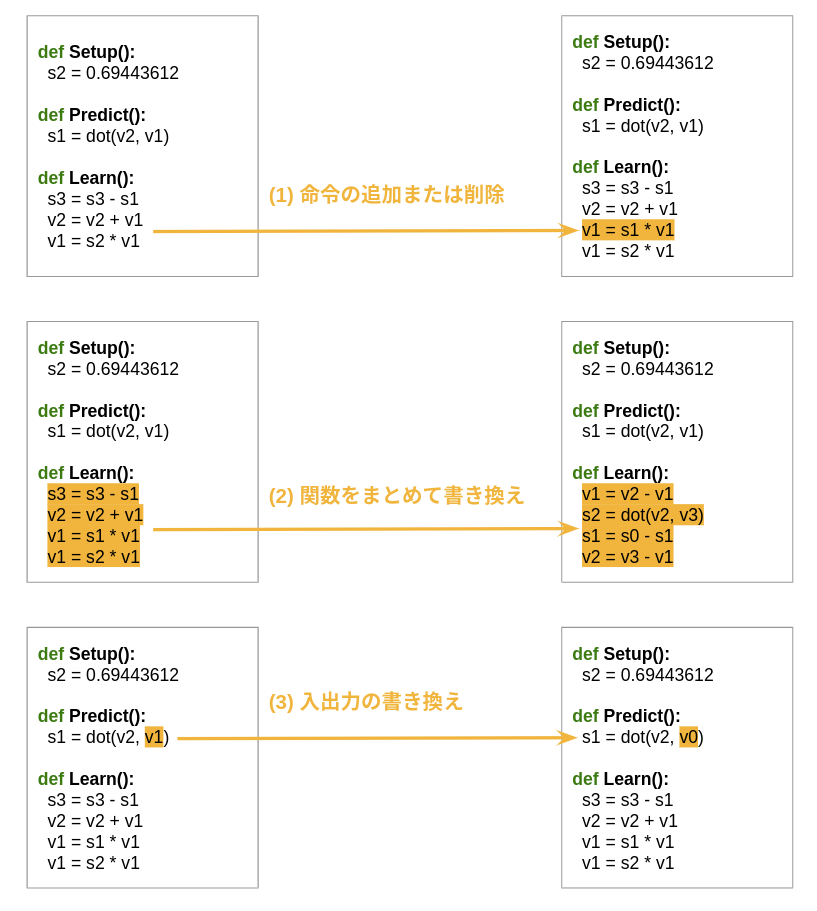
\includegraphics[width=10cm]{problem/existing_method/mutation.png}
  \caption{突然変異の種類\cite{automl_zero}. (1) アルゴリズムのSetup, Predict, Learnのいずれかをランダムに選択した上で, ランダムに命令を追加または削除する. (2) アルゴリズムのSetup, Predict, Learnのいずれかをすべてランダムな命令列で書き換える. (3) アルゴリズム内のいずれかの命令の入出力をランダムに変更する. }
  \label{fig:re_automl_zero:mutation}
\end{figure}

RE-AutoML-Zeroの突然変異は図\ref{fig:re_automl_zero:mutation}に示した3種類が存在する. それぞれの突然変異手法の以下で説明する.

\begin{enumerate}
  \renewcommand{\labelenumi}{(\arabic{enumi})}
  \item Setup関数, Predict関数, Learn関数のいずれかを一様ランダムに選択した上で, 選択された関数に対して命令の追加または削除を行う突然変異. 追加または削除する場所も一様ランダムに決まる.
  \item Setup関数, Predict関数, Learn関数のいずれかを, ランダムな命令列で書き換える突然変異. 命令数は元の個数と変更しない.
  \item Setup関数, Predict関数, Learn関数のいずれかを選択した上で, その関数の1つの命令の入力, 出力もしくは即値のいずれかをランダムに変更する突然変異.
\end{enumerate}
\noindent
突然変異はユーザが与える制限を満たす範囲でのみ行うことができる. RE-AutoML-Zeroのユーザは, Setup関数, Predict関数, Learn関数のそれぞれに対して, 命令数の下限および上限, 命令の種類を指定することができる, また, スカラー, ベクトル, 行列それぞれの仮想メモリのアドレス数も指定可能である. そのため, (1)によってユーザが設定した命令数の上限を超えた追加や下限を下回る削除を行ったり, (2)によって許可されていない命令を関数に追加することは出来ない. また, 仮想メモリ上のスカラーの変数の個数が3個と決まっている場合, すなわち$s0$から$s2$まで使える場合に, (3)で命令の入力変数として$s4$に設定することはできない.

\section{既存手法の問題点}\label{sec:problem:existing_problem}

EstebanらのAutoML-Zeroは人間の事前知識や介入を最小限に抑えつつ機械学習アルゴリズムを自動探索するという画期的な成果を示した一方で, その探索効率には重要な課題が残されている. 例えば, ReLU関数の再発明に成功し, CIFAR-10やMNISTデータセットに対する分類アルゴリズムを発見したSection 4.2の実験では, 膨大な計算リソースが必要とされた. 具体的には, 1秒間あたり10,000モデルの評価が可能なCPUを搭載したマシンを10,000台使用し, 約5日間, 評価回数にして$10^{12}$オーダーの計算を実行している. このような大規模な計算リソースの要求は, 現実的な環境下での応用可能性を制限していると考えられる.

我々は, 既存手法の探索効率を低下させ得る問題として, 探索空間の冗長性に関する問題, 良質な構造を子個体に継承できない問題, 集団の多様維持に関する問題に着目した. 以下, 第\ref{subsec:problem:existing_problem:space}節で探索空間の冗長性に関する問題, 第\ref{subsec:problem:existing_problem:mutation}節で良質な構造を子個体に継承できない問題, 第\ref{subsec:problem:existing_problem:diversity}節で集団の多様維持に関する問題について説明する.

\subsection{探索空間の冗長性に関する問題}\label{subsec:problem:existing_problem:space}

AutoML-Zeroでは, アルゴリズムの評価をする際に, $\mathcal{T}_\mathrm{search}$に含まれる全ての機械学習タスクを解く必要があり多くの時間を要するため, 冗長な探索空間は探索効率を大きく低下させる要因になる. 既存手法には, 変数名の違いによる冗長性, 命令の実行順の違いによる冗長性, 非妥当なアルゴリズムによる冗長性の3つの冗長性が存在すると考えられる. 本節では, それぞれの冗長性について詳しく説明する.

\subsubsection{変数名の違いによる冗長性}
既存手法には, 変数名の違いによる冗長性が存在すると考えられる. 例えば, アフィン回帰と解釈可能なアルゴリズムであるCode.\ref{code:affine_algorithm}において, $s6$という変数が$s8$に変わったり, $v6$が$v1$に変わっても実行結果は同じである. 既存手法では, 実行結果に違いがなく, 変数名が異なるアルゴリズムを区別して探索しているため, 探索空間が冗長になっていると考えられる.

\subsubsection{命令の実行順の違いによる冗長性}
既存手法には, 命令の実行順の違いによる冗長性が存在すると考えられる. 例えば, アフィン回帰と解釈可能なアルゴリズムであるCode.\ref{code:affine_algorithm}において, 12行目と13行目が入れ替わっても実行結果は同じである. 既存手法では, 実行結果に違いがなく, 命令の順序が異なるアルゴリズムを区別して探索しているため, 探索空間が冗長になっていると考えられる.

\subsubsection{非妥当なアルゴリズムによる冗長性}

既存手法は, 機械学習アルゴリズムとして妥当ではないアルゴリズムが探索対象となっており, 探索空間が冗長になっているという問題が存在する. ここで, 妥当ではないアルゴリズムとは, 以下の妥当なアルゴリズムの条件のいずれかを満たさないアルゴリズムである.

\begin{enumerate}
  \item Learn関数で逐次更新される全ての学習パラメータが以下の条件を満たすこと.
  \begin{enumerate}
    \item 1ステップ前の自分自身の値に依存して更新されていること
    \item Predict関数で利用されている場合は, 正解ラベル$s0$に依存して更新されていること.
    \item Predict関数で利用されている場合は, 予測ラベル$s1$に依存して更新されていること.
  \end{enumerate}
  \item Predict関数で予測ラベル$s1$の算出に, 以下が利用されていること.
  \begin{enumerate}
    \item 入力ベクトル$v0$
    \item 1つ以上のLearn関数で逐次更新される学習パラメータ
  \end{enumerate}
  \item 全ての変数が最終的に予測ラベル$s1$の算出に寄与すること.
\end{enumerate}

これらの条件は, 機械学習タスクを高い適合度で解くために, タスクの種類によらず普遍的に必要不可欠な性質である. そのため, 妥当なアルゴリズムの条件を満たさないアルゴリズムを探索することは非効率的である. しかし, 既存手法ではこれらの条件を考慮せずに, 全てを探索しているため, 探索空間に冗長性が生じていると考えられる.

妥当なアルゴリズムの例をCode.\ref{code:valid_algorithm}に, 既存手法で探索対象となっている妥当ではないアルゴリズムの例と妥当ではない理由をCode.\ref{code:invalid_algorithm_1}からCode.\ref{code:invalid_algorithm_7}に示す.

\begin{multicols}{2}
  \begin{lstlisting}[caption=妥当な機械学習アルゴリズムの例,label=code:valid_algorithm]
  def Setup():
    s2 = 0.01

  def Predict():
    s1 = dot(v1, v0)

  def Learn():
    s3 = s0 - s1
    s3 = s2 * s3
    v2 = s3 * v0
    v1 = v1 + v2
  \end{lstlisting}

  \columnbreak

  \begin{lstlisting}[caption=妥当なアルゴリズムの条件4を満たさない非妥当なアルゴリズム,label=code:invalid_algorithm_1]
  def Setup():
    s2 = 0.01

  def Predict():
    <@\red{s2}@> = dot(v1, v0)

  def Learn():
    s3 = s0 - s1
    s3 = s2 * s3
    v2 = s3 * v0
    v1 = v1 + v2
\end{lstlisting}
\end{multicols}

\begin{multicols}{2}
  \begin{lstlisting}[caption=妥当なアルゴリズムの条件2の(a)を満たさない非妥当なアルゴリズム,label=code:invalid_algorithm_2]
    def Setup():
      s2 = 0.01

    def Predict():
      s1 = dot(v1, <@\red{v3}@>)

    def Learn():
      s3 = s0 - s1
      s3 = s2 * s3
      v2 = s3 * v0
      v1 = v1 + v2
  \end{lstlisting}

  \columnbreak

  \begin{lstlisting}[caption=妥当なアルゴリズムの条件2の(b)を満たさない非妥当なアルゴリズム,label=code:invalid_algorithm_3]
    def Setup():
      s2 = 0.01

    def Predict():
      s1 = dot(<@\red{v3}@>, v0)

    def Learn():
      s3 = s0 - s1
      s3 = s2 * s3
      v2 = s3 * v0
      v1 = v1 + v2
  \end{lstlisting}
\end{multicols}

\newpage

\begin{multicols}{2}
  \begin{lstlisting}[caption=妥当なアルゴリズムの条件1の(a)を満たさない非妥当なアルゴリズム,label=code:invalid_algorithm_4]
    def Setup():
      s2 = 0.01

    def Predict():
      s1 = dot(v1, v0)

    def Learn():
      s3 = s0 - s1
      s3 = s2 * s3
      v2 = s3 * v0
      v1 = <@\red{v0}@> + v2
  \end{lstlisting}

  \columnbreak

  \begin{lstlisting}[caption=妥当なアルゴリズムの条件1の(b)を満たさない非妥当なアルゴリズム,label=code:invalid_algorithm_5]
    def Setup():
      s2 = 0.01

    def Predict():
      s1 = dot(v1, v0)

    def Learn():
      s3 = <@\red{s2}@> - s1
      s3 = s2 * s3
      v2 = s3 * v0
      v1 = v1 + v2
  \end{lstlisting}
\end{multicols}

\begin{multicols}{2}
  \begin{lstlisting}[caption=妥当なアルゴリズムの条件1の(c)を満たさない非妥当なアルゴリズム. ,label=code:invalid_algorithm_6]
    def Setup():
      s2 = 0.01

    def Predict():
      s1 = dot(v1, v0)

    def Learn():
      s3 = s0 - <@\red{s2}@>
      s3 = s2 * s3
      v2 = s3 * v0
      v1 = v1 + v2
  \end{lstlisting}

  \columnbreak

  \begin{lstlisting}[caption=妥当なアルゴリズムの条件3を満たさない非妥当なアルゴリズム,label=code:invalid_algorithm_7]
    def Setup():
      s2 = 0.01

    def Predict():
      s1 = dot(v1, v0)

    def Learn():
      s3 = s0 - s1
      <@\red{s4}@> = s2 * s3
      v2 = s3 * v0
      v1 = v1 + v2
  \end{lstlisting}
\end{multicols}

\subsection{良質な構造を子個体に継承できない問題}\label{subsec:problem:existing_problem:mutation}

既存手法の突然変異の2つの問題によって, 既存手法では良質な構造を子個体に継承できない問題が存在すると考えられる. 一つは, 親個体が妥当なアルゴリズムであっても, 既存手法の突然変異によって非妥当なアルゴリズムに変化してしまう確率が高い点である. もう一つは突然変異の局所性に関する課題である. 本節では, それぞれについて説明する.

\subsubsection{非妥当なアルゴリズムに高確率で突然変異する問題}
既存手法では, 親個体が妥当なアルゴリズムであったとしても, 妥当ではないアルゴリズムに変化させてしまう妥当ではない突然変異が頻発する問題が存在する. 実際, 予備実験の結果により, 妥当な線形回帰アルゴリズムを突然変異させると, 98\%以上の確率で妥当ではないアルゴリズムに変化することが確かめられている. これによって, 妥当ではないアルゴリズムが大量に評価されてしまい, 探索効率が低下していると考えられる.

\subsubsection{突然変異の局所性に関する問題}
既存手法では, (1)の単一命令の追加・削除や(3)の変数アドレスの変更といった局所的な突然変異と(2)の関数全体をランダムに変更する破壊的な突然変異が実装されている. 局所的な突然変異のみでは, アルゴリズム構造を大きく変更することはない一方で, 十分な探索空間を探索することが難しい. しかしながら, (2)のような関数内のアルゴリズムを全て変える破壊的な突然変異は, 関数中の良質な部分命令列が存在していたとしても, 子個体にその良質な部分命令列が継承ができなくなってしまう可能性が高い. 故に, 既存手法の子個体生成方法では, 関数中の良質な部分命令列を保存しつつ, 関数を逐次改善することが難しいと考えられる.

\subsection{集団の多様性維持に関する問題}\label{subsec:problem:existing_problem:diversity}

既存手法には, 多様性維持に関する問題として, 世代交代モデルREの問題, 集団に同一個体が存在する問題, 個体の希少性が無視される問題が存在すると考えられる. 多様性維持の困難さにより, 既存手法は探索序盤で発見された局所最適なアルゴリズムに早期収束してしまい, 探索効率の低下を招いていると考えられる.

\subsubsection{世代交代モデルREに関する問題}

既存手法のRE-AutoML-Zeroで採用されている世代交代モデルであるREは, 集団の多様性を失いやすいと考えられる. 佐藤らの論文\cite{mgg}の考察を踏まえると, REが集団の多様性を低下させる要因として, 主に以下の3点が考えられる.

\begin{enumerate}
  \item Fig.\ref{fig:regularized_evolution}のSTEP1 (Algorithm \ref{algorithm:re_automl_zero}の11行目)において, 無条件で元の集団の個体が淘汰されている点
  \item Fig.\ref{fig:regularized_evolution}のSTEP2 (Algorithm \ref{algorithm:re_automl_zero}の12行目)における複製選択で, 強い選択圧が掛かるトーナメント選択が用いられている点
  \item Fig.\ref{fig:regularized_evolution}のSTEP3およびSTEP4(Algorithm \ref{algorithm:re_automl_zero}の13行目から19行目)における生存選択で選ばれる個体が淘汰される個体と無関係である点
\end{enumerate}

\noindent
1つめは, 希少な構造を持つ個体も無条件で淘汰されることを意味しており, 多様性の低下を招くと考えられる. 2つめは, 探索序盤で得られた局所最適解に対しても選択圧が強く掛かることを意味しており, 十分な探索をする前に多様性を低下させる恐れがある. 3つめは, 淘汰される個体の形質が次世代に引き継げなくなることを意味しており, 集団の多様性を低下させる要因になると考えられる. 実際, これらの要因によって, 集団の多様性維持が困難になり, 探索に要す評価回数が増加したり, 局所最適解に陥りやすくなることが佐藤らの論文\cite{mgg}でも示されている.

\subsubsection{集団に同一個体が存在する問題}

既存手法のRE-AutoML-Zeroは, 既に集団内に存在する個体と同等の個体が初期個体や子個体生成時に追加される問題が存在する. 集団内に同等のアルゴリズムが追加されると, 相対的に希少な構造を持つ個体が淘汰される可能性が高まり, 集団の多様性が維持しにくくなると考えられる.

\subsubsection{個体の希少性が考慮されていない問題}

既存手法では, 個体の希少度を考慮せずに世代交代を行なっており, 仮に改善の見込みがある良質な構造を持つアルゴリズムが生成されたとしても, 他の数が多い局所最適なアルゴリズムによって淘汰されてしまい, 集団の多様性が低下してしまうと考えられる.

\chapter{提案手法}\label{chap:proposed}

\section{基本的な考え方}

提案手法では, 既存手法の問題点として挙げた探索空間の冗長性, 個体の良質な構造を子個体に継承できない問題, 集団の多様性維持に関する問題に対処した手法を提案する. RE-AutoML-Zeroの人間の事前知識や介入を最小限にできる利点は残しつつ, 探索効率を向上させることを目指す.

探索空間の冗長性については, グラフ構造によるアルゴリズムの表現(アルゴリズムグラフ)を導入することで対処する. アルゴリズムグラフは, 付録\ref{chap:ordered_directed_graph}で示した閉路を持たない順序付き有向グラフであり, 各ノードには, 命令, 定数値, 入力ベクトル, 正解ラベル, および学習過程で逐次更新される学習パラメータが割り当てられる. 命令ノードの子ノードに命令の入力に対応するノードを配置することで, アルゴリズムの依存関係を表現する. グラフ構造を用いることで, 変数名や実行順が異なるだけで実行結果は同じアルゴリズムを同一視することが可能となり, 変数名や命令の順序による冗長性の削減が可能となる. その上で, アルゴリズムグラフに対して, 機械学習アルゴリズムとして満たすべき条件(妥当なアルゴリズムの条件)を明確に規定し, 条件を満たさないアルゴリズムを探索空間から除外する. これにより, 非妥当なアルゴリズムによる探索空間の冗長性についても対処する.

個体の良質な構造を子個体に継承できない問題には, アルゴリズムグラフを用いた突然変異によって対処する. 提案手法の突然変異では, アルゴリズムの妥当性を引き継げない非妥当な突然変異が起こらないように保証する. その上で, 部分グラフの再構成を用いた新たな突然変異を導入することで, 関数内の特定の変数の計算に利用する部分命令列のみを変化させる子個体生成を実現する. これによって, 第\ref{subsec:problem:existing_problem:mutation}節で述べた関数全体をランダムに書き換える破壊的な突然変異を抑制することができ, 少ない評価回数で高い適合度のアルゴリズムを発見できることが期待できる.

集団の多様性維持に関する問題には, Minimal Generation Gap (MGG) \cite{mgg}による世代交代モデル, 集団内の同一個体の排除および希少度に基づく生存選択を導入することで対処する. 佐藤らの考察を踏まえると, MGGは既存手法のREに比べて, 集団の多様性を維持しやすい世代交代モデルと考えられる\cite{mgg}. また, 集団内に同一個体や類似個体が増えてしまうと, 探索の初期段階で局所最適なアルゴリズムに陥ってしまうため, 同一個体が集団に追加されないようにした上で, 個体の希少度を考慮した世代交代を実現する. これにより, 探索が進んでいない段階で, 有望な個体を淘汰させる可能性が減少し, 局所最適なアルゴリズムに陥る問題を解決できると考えられる.

本章では, 第\ref{sec:proposed:ag}節で, アルゴリズムグラフの定義と評価, 探索空間を削減するために必要となる妥当なアルゴリズムの条件, 個体の生成や世代交代に必要となるアルゴリズムグラフのノードに対するNLP媒介数や同一性の概念について説明する. その後, 第\ref{sec:proposed:initialization}節で, 提案手法における初期集団の生成方法, 第\ref{sec:proposed:mutation}節で既存手法の問題点に対処した突然変異を導入した子個体生成方法について説明する. 最後に, 第\ref{sec:proposed:diversity}節で, 集団の多様性を維持するために必要な世代交代モデルMGG, 集団内の同一個体の排除, 希少度に基づく生存選択について述べる.

\section{アルゴリズムグラフ (AG)}\label{sec:proposed:ag}

本節では, 提案手法の機械学習アルゴリズムの表現形式であるアルゴリズムグラフ (Algorithm Graph, AG) について論じる. AGは, 閉路を持たない順序付き有向グラフであり, 各ノードには, 命令, 定数値, 入力ベクトル, 正解ラベル, および学習過程で逐次更新される学習パラメータが割り当てられる. 命令ノードの子ノードに命令の入力に対応するノードを配置することで, アルゴリズムの依存関係を表現する. AGを用いると, 変数名や実行順序の異なる同値なアルゴリズムを一意に表現でき, 探索空間の冗長性を削減可能である. さらに, AGにおける妥当なアルゴリズムの条件を定式化し, 妥当なアルゴリズムグラフ (Valid Algorithm Graph, VAG)のみを探索対象とすることで, 非妥当なアルゴリズムに起因する冗長性も合わせて削減する.

本節では, 第\ref{subsec:proposed:ag:exp}節でAGの定義, 第\ref{subsec:proposed:ag:eval}節でAGの評価, 第\ref{subsec:proposed:ag:redundancy}節でAGで削減できる探索空間の冗長性, 第\ref{subsec:proposed:ag:vag}節でVAGについて述べる. その後, 第\ref{subsec:proposed:ag:nlp_count}節で, VAGの個体を生成するために必要となるノードのNLP媒介数を定義する. 最後に, 第\ref{subsec:proposed:ag:equivalent}節で提案手法の世代交代モデルで必要となるAGの同一性と構造的同一性について述べる.

\subsection{AGの定義}\label{subsec:proposed:ag:exp}
本論文では, アルゴリズムグラフを非巡回順序付き有向グラフ$G = (U, E)$として定式化する. ここで, $U$はノードの集合, $E \subset U \times \mathbb{N} \times U$は順序エッジの集合である. 順序エッジ$(u_1, n, u_2)$は通常の有向グラフのエッジとは異なり, 始点$u_1$と終点$u_2$の他に, $u_1$の何番目のエッジであるかを表す順序値$n \in \mathbb{N}$を持つ. 非巡回順序付き有向グラフの詳細は, 付録\ref{chap:ordered_directed_graph}を参照されたい.

アルゴリズムグラフ$G = (U, E)$のノード集合$U$に属する各ノードは, 以下の4つの型のいずれかに分類される.

\begin{description}
  \item[定数ノード] \ \\ 定数値を表すノードでスカラー, ベクトル, 行列のいずれかの定数値が格納されている.
  \item[データノード]\ \\ 学習データや検証データの代入先となるノードであり, 以下の2つが存在する.
  \begin{description}
    \item[入力ベクトルノード: $u_\mathrm{f}$] \ \\ 学習データや検証データの入力ベクトルを代入するノード. $U$の中にただ一つのみ存在し, $u_\mathrm{f}$と表す. 第\ref{subsec:problem:existing_method:algorithm_exp}節で述べた既存手法のアルゴリズムの表現における$v0$に対応する.
    \item[正解ラベルノード: $u_\mathrm{c}$] \ \\ 学習データの正解ラベルを代入するノード. $U$の中にただ一つのみ存在し, $u_\mathrm{c}$と表す. 第\ref{subsec:problem:existing_method:algorithm_exp}節で述べた既存手法のアルゴリズムの表現における$s0$に対応する.
  \end{description}
  \item[LPノード: $u_{\mathrm{lp},i}$] \ \\ 学習時に逐次更新される学習パラメータ (Learning Parameter, LP) を表すノード. 学習時の最初のステップでは, 当該学習パラメータの初期値が格納されており, それ以降のステップでは, 1ステップ前で更新された値が格納されている. 一般に複数存在するため, 順序をつけて$u_{\mathrm{lp},i}$と表す.
  \item[命令ノード] \ \\ Table.\ref{table:instructions}に示した命令セット内の命令が割り当てられたノード. 命令の入力に対応するノードを子ノードとして持ち, 命令の出力値が格納されている. $n$番目の子ノードが第$n$引数に対応する. また, 出力の利用用途が特殊な命令ノードとして, 以下の予測ノードとNLPノードが存在する.
  \begin{description}
    \item[予測ノード: $u_{p}$] \ \\ 出力が予測ラベルとして利用される特殊な命令ノード. ノード集合の$U$内にただ一つのみ存在し, $u_{p}$と表す. 第\ref{subsec:problem:existing_method:algorithm_exp}節で述べた既存手法のアルゴリズムの表現における$s1$に対応する. また, 予測に正解ラベルを利用することはできないため, 予測ノードの子孫ノードに正解ラベルノードを含めることはできない.
    \item[NLPノード: $u_{\mathrm{nlp},i}$] \ \\ 出力が次のステップの特定の学習パラメータ (Next Learning Parameter, NLP) の値として利用される特殊な命令ノード. NLPノードは, $U$内にLPノードと同様の個数存在し, NLPノードとLPノードは1対1で対応するため, 添え字を対応させて$u_{\mathrm{nlp},i}$と表す.
  \end{description}
\end{description}
\noindent
これらのノードのうち, 子ノードを持つノードは命令ノードのみであり, それ以外のノードは子ノードを持たない. そのため, 定数ノード, 入力ベクトルノード, 正解ラベルノード, LPノードをまとめて終端ノードと呼ぶ. また, 各ノードにはスカラー型, ベクトル型, 行列型のいずれかが割り当てられており, 命令ノードの子ノードを割り当てる際は, 命令の入力の型の整合性が保たれる必要がある.

AGにおける1つの命令ノードとそのノードを始点とするエッジは, 第\ref{subsec:problem:existing_method:algorithm_exp}節で述べた既存手法のアルゴリズムの表現における1行と対応する. 例えば, Fig.\ref{fig:mgg_automl_zero_vag:op_node}に示した命令ノード$u_\mathrm{op} \in U$と2つのエッジ$(u_\mathrm{op}, 1, u_\mathrm{c})$と$(u_\mathrm{op}, 2, u_\mathrm{p})$は, Code.\ref{code:affine_algorithm_proposed}の9行目の命令$s4 = s0 - s1$と対応しており, $u_\mathrm{op}$は$s4$, $s0$は正解ラベルノード$u_\mathrm{c}$, $s1$は予測ノード$u_\mathrm{p}$に対応する.

アフィン回帰と解釈可能なアルゴリズムCode.\ref{code:affine_algorithm}のAGをFig.\ref{fig:mgg_automl_zero_vag:affine}に示す. 図において, 命令ノードは円形, 定数ノードは四角形, データノードはひし形, LPノードは台形で表現されている. 特殊な命令ノードである予測ノードとNLPノードは二重丸で示した. また, 対応関係にあるLPノードとNLPノードは同じ色で着色した. 命令ノードには, 割り当てられている命令の演算子, 定数ノードには代入されている定数値, LPノードには学習パラメータの初期値が記載されている. 子ノードを持つノードの場合は, 図の上部にある子ノードを順序値が小さいものとする. また, アルゴリズムグラフでは不要ではあるが, Code.\ref{code:affine_algorithm}との対応関係を明確にするために, 各ノードには代入先の変数名を記載している.

\begin{figure}[t]
\begin{lstlisting}[caption=アフィン回帰と解釈可能なアルゴリズム (Code.\ref{code:affine_algorithm}と同様),label=code:affine_algorithm_proposed]
  def Setup():
    s3 = 0.01 // 学習率の設定

  def Predict():
    s2 = dot(v6, v0) // 重みと入力ベクトルの内積を計算
    s1 = s7 + s2 // 切片を加算

  def Learn():
    s4 = s0 - s1 // 予測ラベルと正解ラベルの誤差を計算
    s6 = s3 * s4 // 学習率の適用
    v3 = s6 * v0 // 傾きの更新するための差分を計算
    v6 = v6 + v3 // 傾きを更新
    s7 = s7 + s6 // 切片を更新
\end{lstlisting}
\end{figure}

\begin{figure}
  \centering
  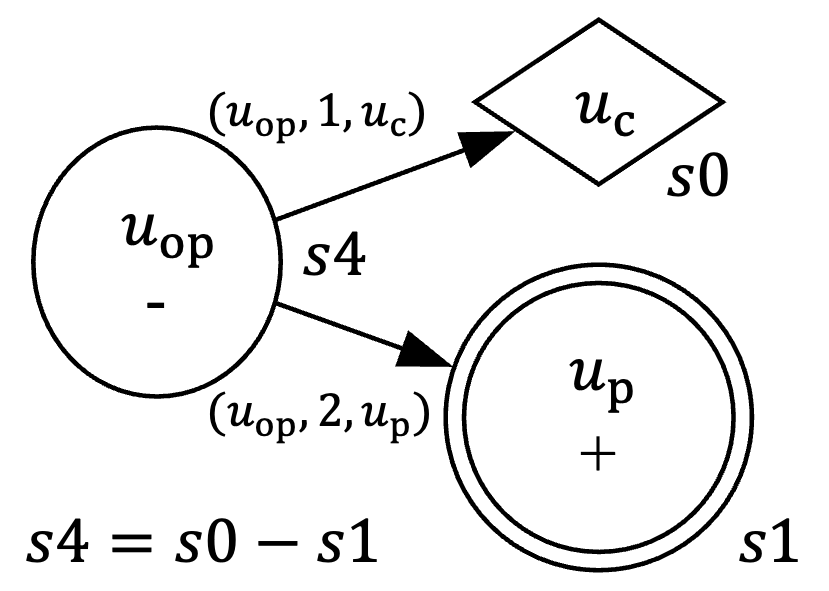
\includegraphics[width=6cm]{mgg_automl_zero_vag/ag/op_node.png}
  \caption{Code.\ref{code:affine_algorithm_proposed}における9行目の命令$s4 = s0 - s1$に対応するAGの命令ノード. $u_\mathrm{op}$は$s4$, $s0$は正解ラベルノード$u_\mathrm{c}$, $s1$は予測ノード$u_\mathrm{p}$に対応する. 後述するFig.\ref{fig:mgg_automl_zero_vag:affine}のAGの例と整合性を取るためにノードを表す図形を区別して利用している. また, 対応関係を分かりやすくするために, 変数名をノードに併記している. }
  \label{fig:mgg_automl_zero_vag:op_node}
\end{figure}

\begin{figure}
  \centering
  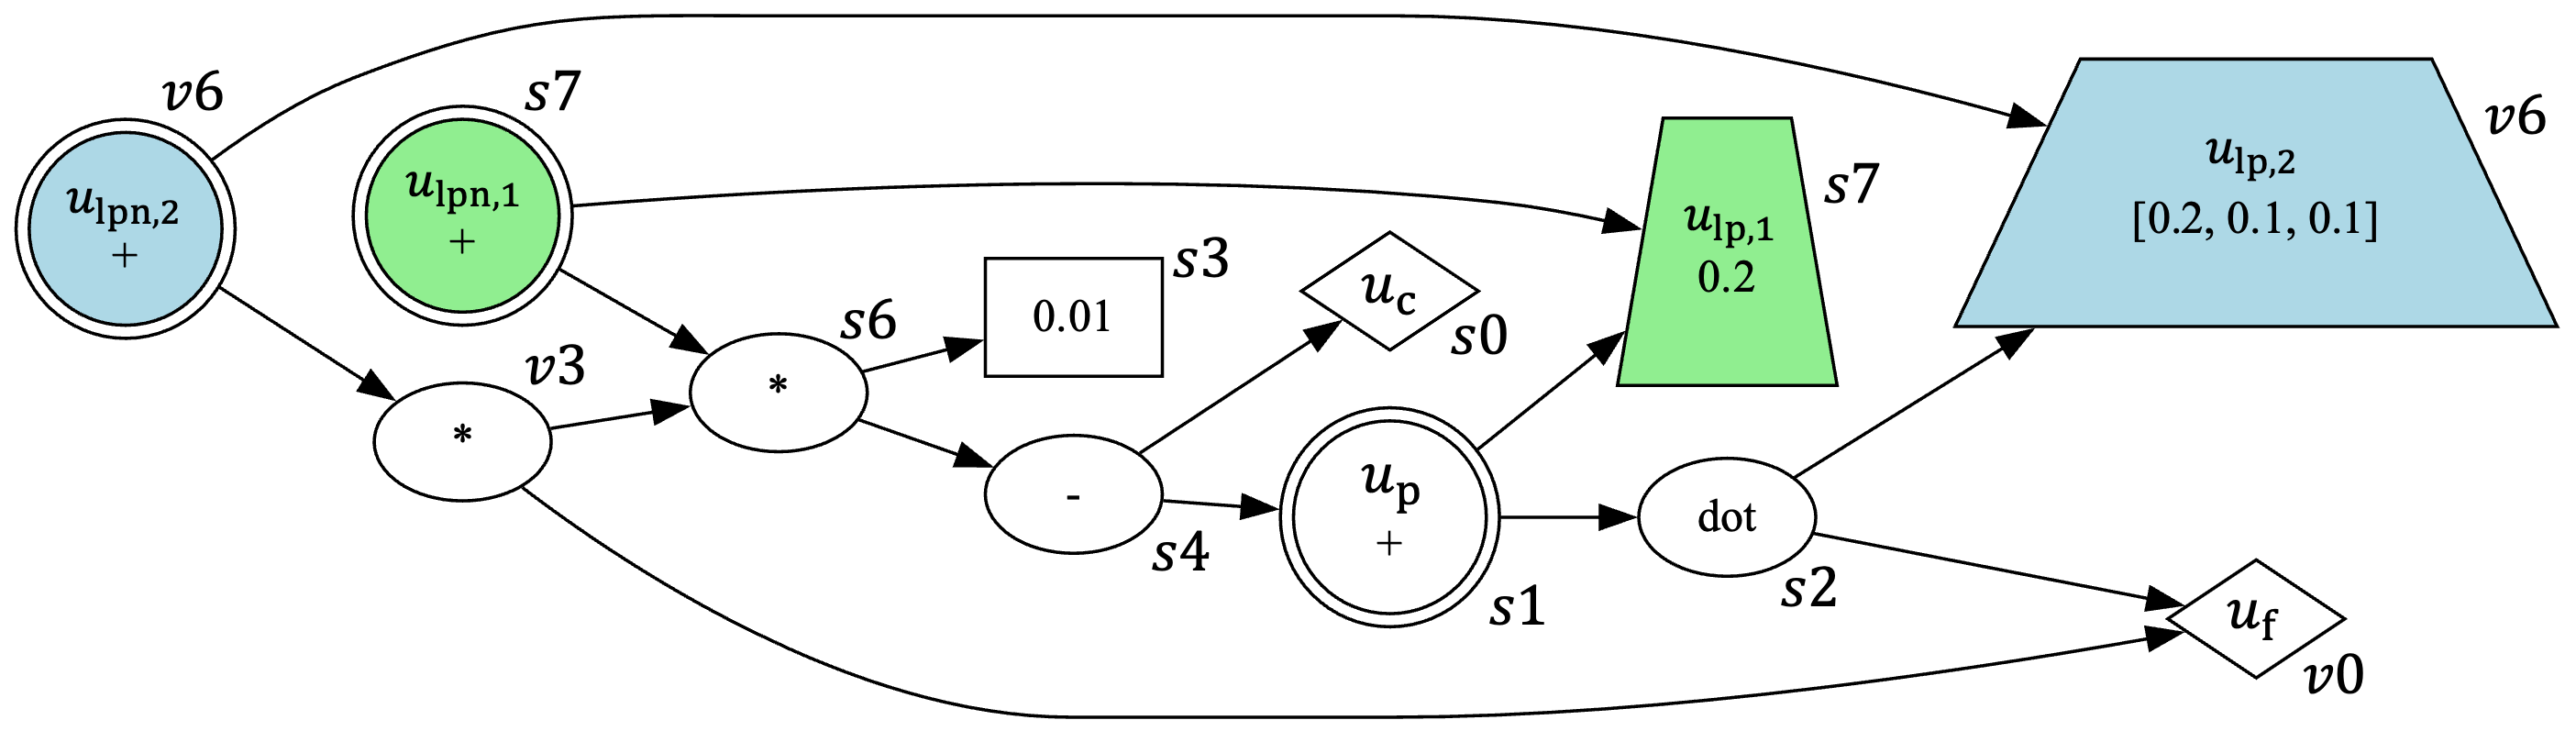
\includegraphics[width=14cm]{mgg_automl_zero_vag/ag/affine.png}
  \caption{アフィン回帰と解釈可能なアルゴリズムCode.\ref{code:affine_algorithm_proposed}のAG.  命令ノードは円形, 定数ノードは四角形, データノードはひし形, LPノードは台形で表現されている. 特殊な命令ノードである予測ノードとNLPノードは二重丸で示した. また, 対応関係にあるLPノードとNLPノードは同じ色で着色した. 命令ノードには, 割り当てられている命令の演算子, 定数ノードには代入されている定数値, LPノードには学習パラメータの初期値が記載されている. 子ノードを持つノードの場合は, 図の上部にある子ノードを順序値が小さいものとする. また, AGでは不要ではあるが, Code.\ref{code:affine_algorithm_proposed}との対応関係を明確にするために, 各ノードには代入先の変数名を併記している. }
  \label{fig:mgg_automl_zero_vag:affine}
\end{figure}

\subsection{AGの評価} \label{subsec:proposed:ag:eval}

AGは, 既存手法の命令列の形式に変換した上で, 第\ref{subsec:problem:existing_method:algorithm_eval}節で述べた既存手法と同様の手法で評価を行う. 変換する際は, 定数ノードの定数の代入とLPノードの初期値の代入をSetup関数に割り当てて, 予測ノードおよびその子孫の命令ノードをPredict関数に割り当てる. また, NLPノードおよびその子孫の命令ノードのうち, Predict関数に割り当てていないノードをLearn関数に割り当てる. 命令ノードを割り当てる際は, 命令の実行順が付録\ref{chap:ordered_directed_graph}に示したトポロジカルソートの逆順になるようにする. これにより, AGで表される依存関係を保持して, 既存手法の表現形式で命令の実行を行うことができる. また, 中間変数に関しては, 特殊な変数$s0$, $s1$, $v0$以外のアドレスを順番に利用する.

機械学習タスクを実行する際の1ステップ分 (1データ分) の処理の流れを, AGに対応させて説明する. Setup関数実行時は, Fig.\ref{fig:mgg_automl_zero_vag:setup}に赤色で示した定数ノードの値とLPノードの初期値が代入される. 予測時には, Fig.\ref{fig:mgg_automl_zero_vag:predict}で示したように, 入力ベクトルノードに入力ベクトルが代入された後で, 赤色で示した命令ノードが数字の順に実行される. 予測ラベルノード$u_\mathrm{p}$の出力値が, 既存手法における予測ラベル$s1$の値として利用される. 学習時には, Fig.\ref{fig:mgg_automl_zero_vag:learn}で示したように, 正解ラベルノードに正解ラベルが代入された後で, 赤色で示した命令ノードが数字の順に実行される. 各NLPノードの出力値は, 次のステップの対応するLPノードの値として利用される.

\begin{figure}
  \centering
  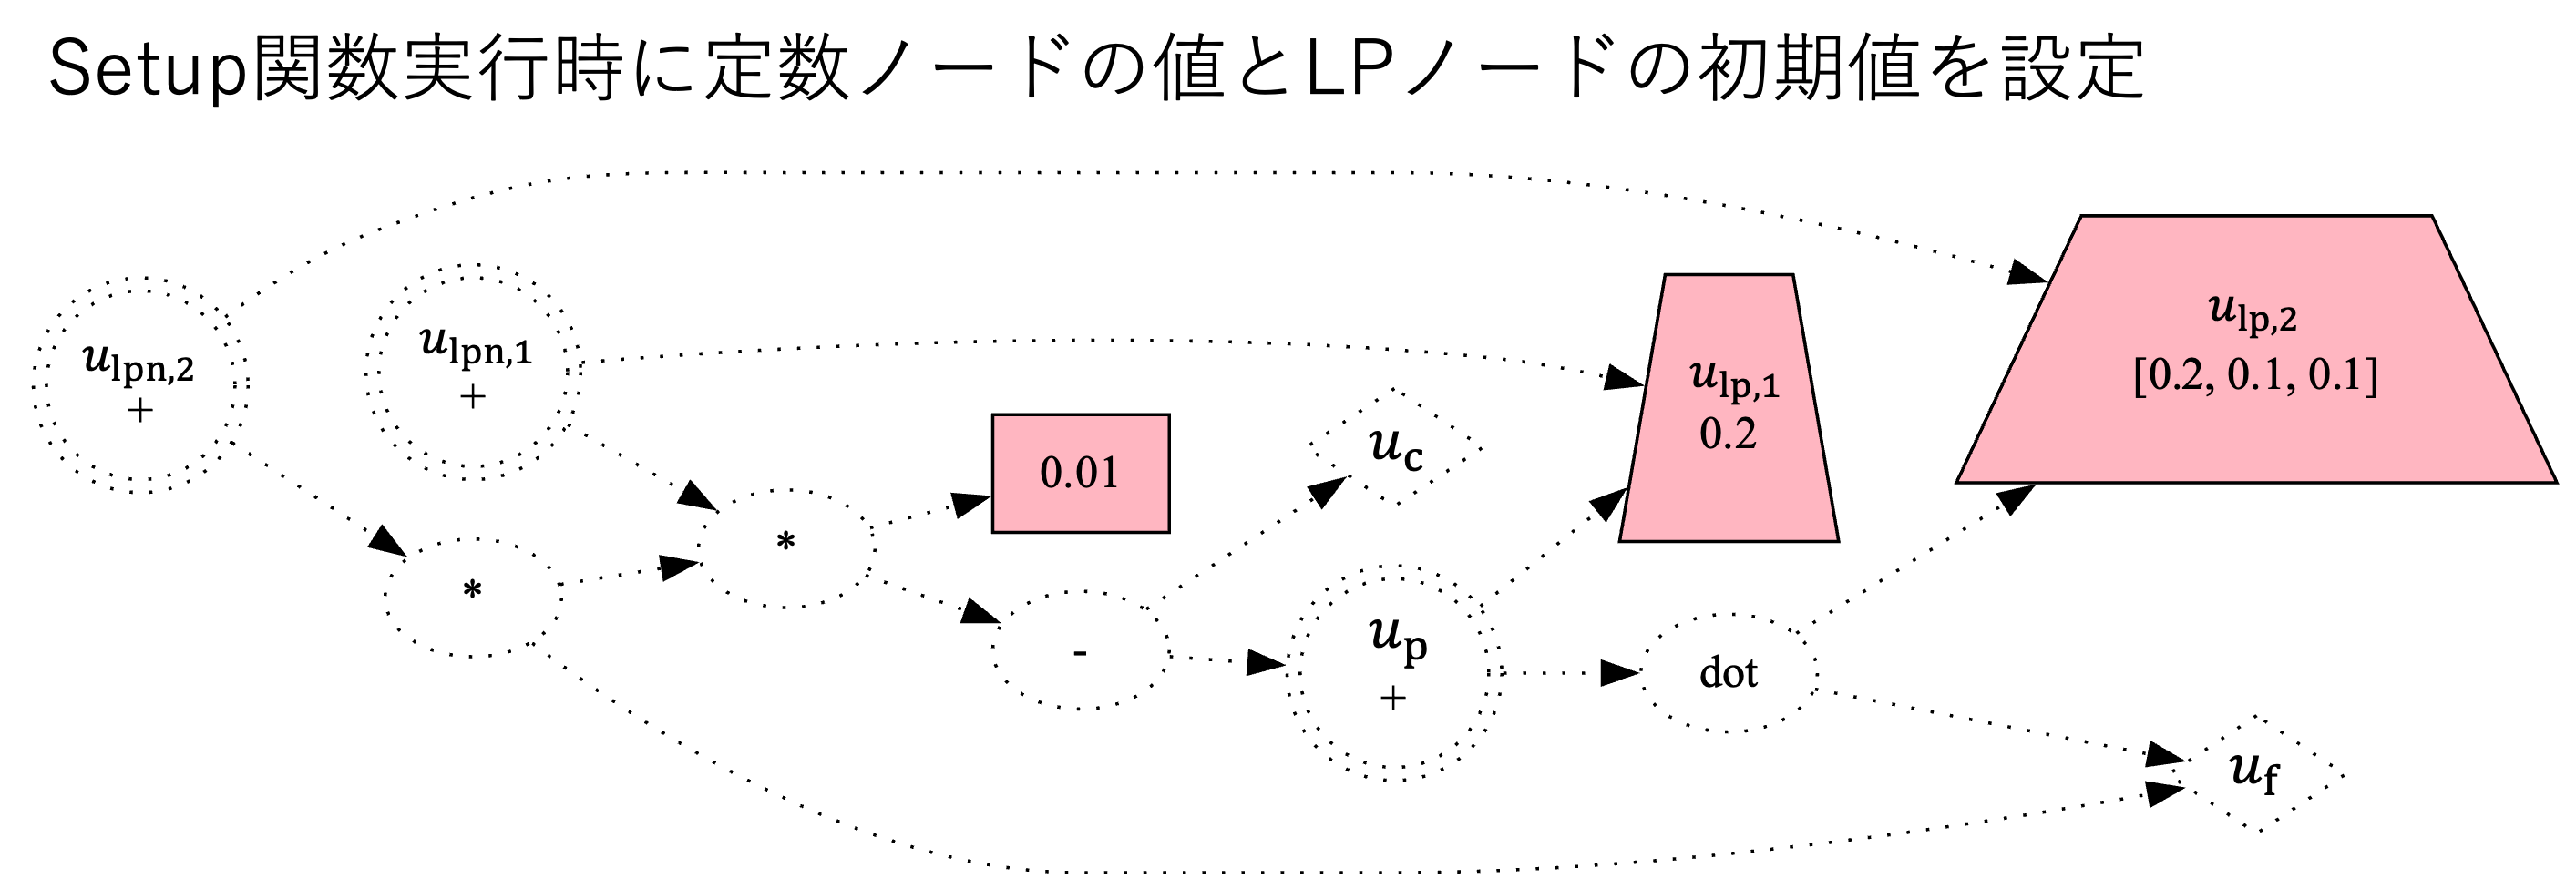
\includegraphics[width=14cm]{mgg_automl_zero_vag/ag/setup.png}
  \caption{Setup関数を実行時のAGの様子. Setup関数では定数ノードの値とLPノードの初期値が代入される. ピンク色で着色したノードがSetup関数内で代入されるノードである. }
  \label{fig:mgg_automl_zero_vag:setup}
\end{figure}
\begin{figure}
  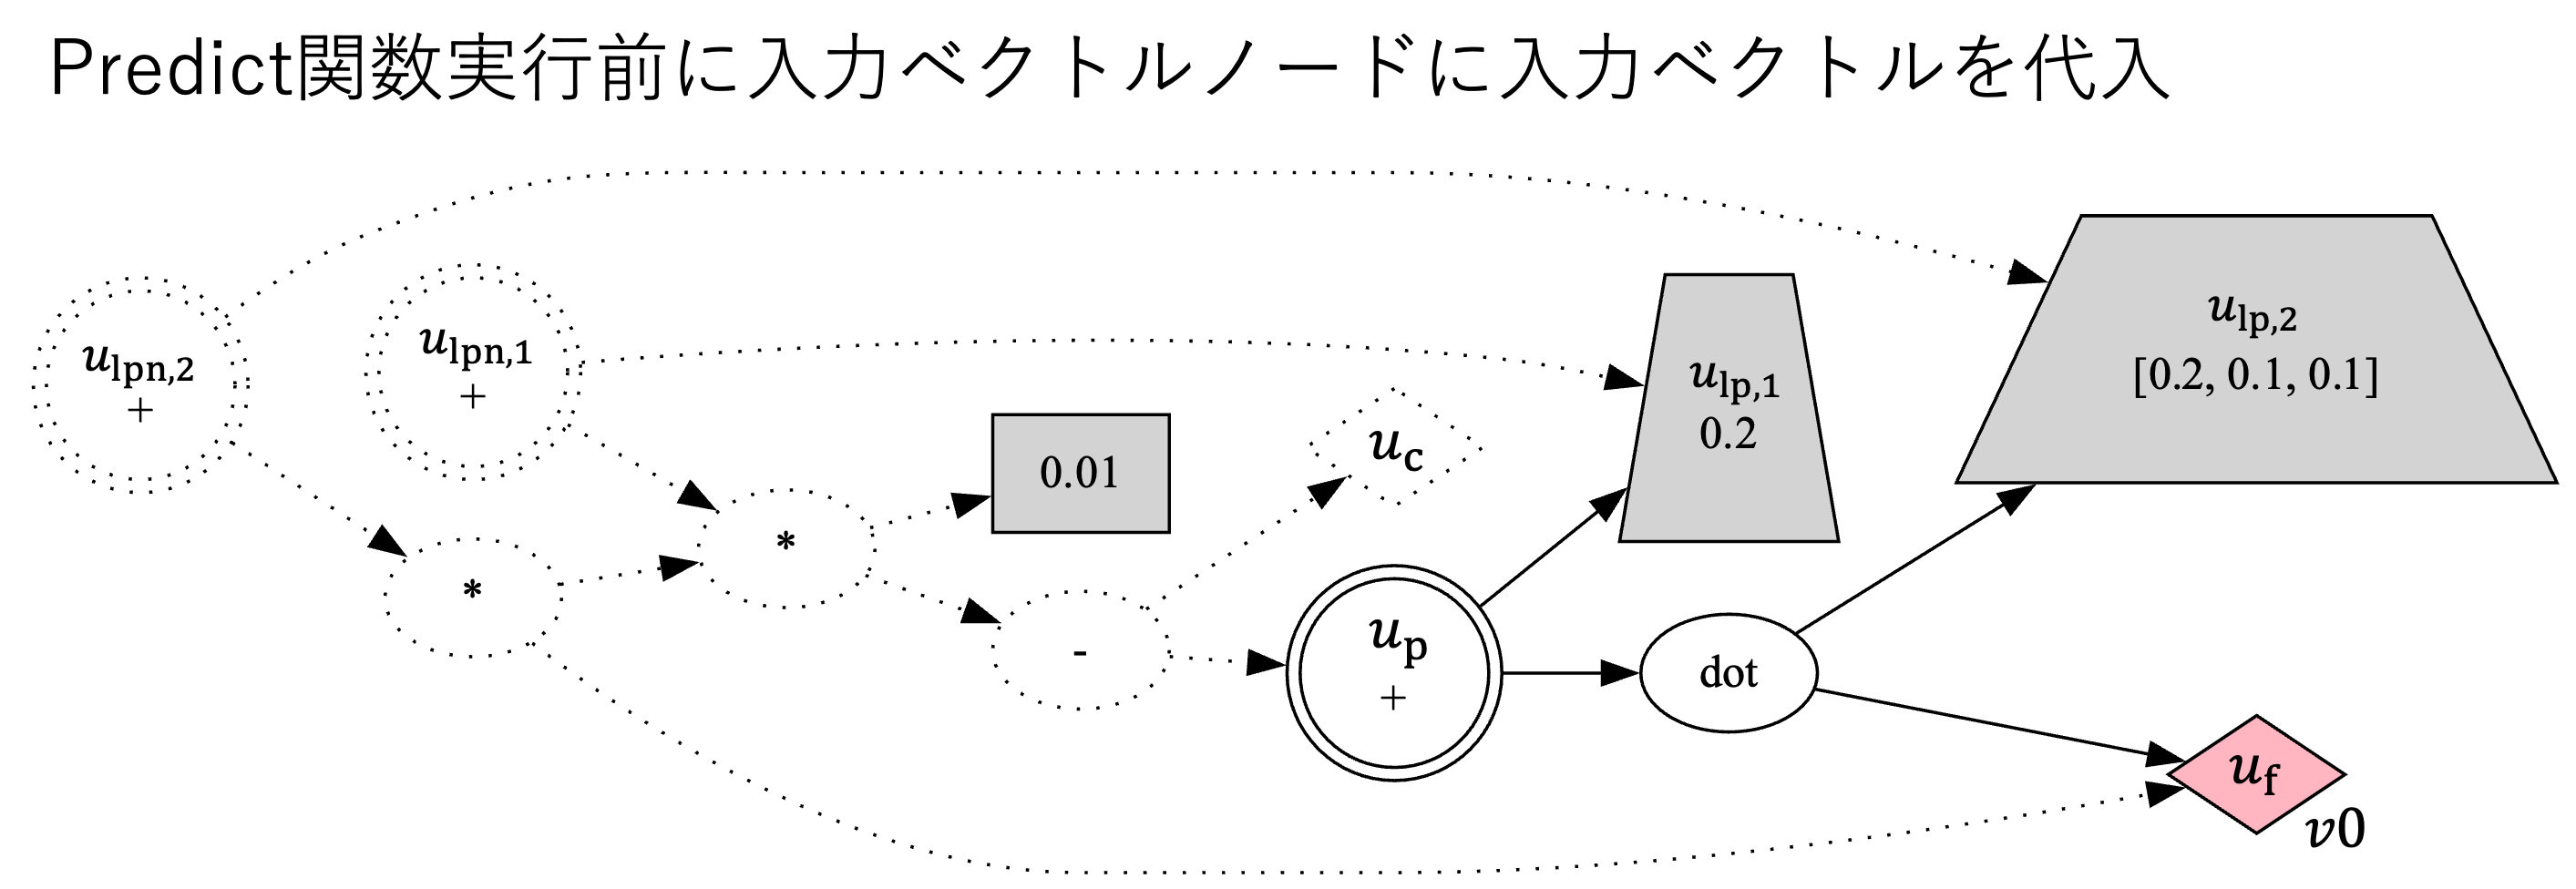
\includegraphics[width=14cm]{mgg_automl_zero_vag/ag/before_predict.png}
  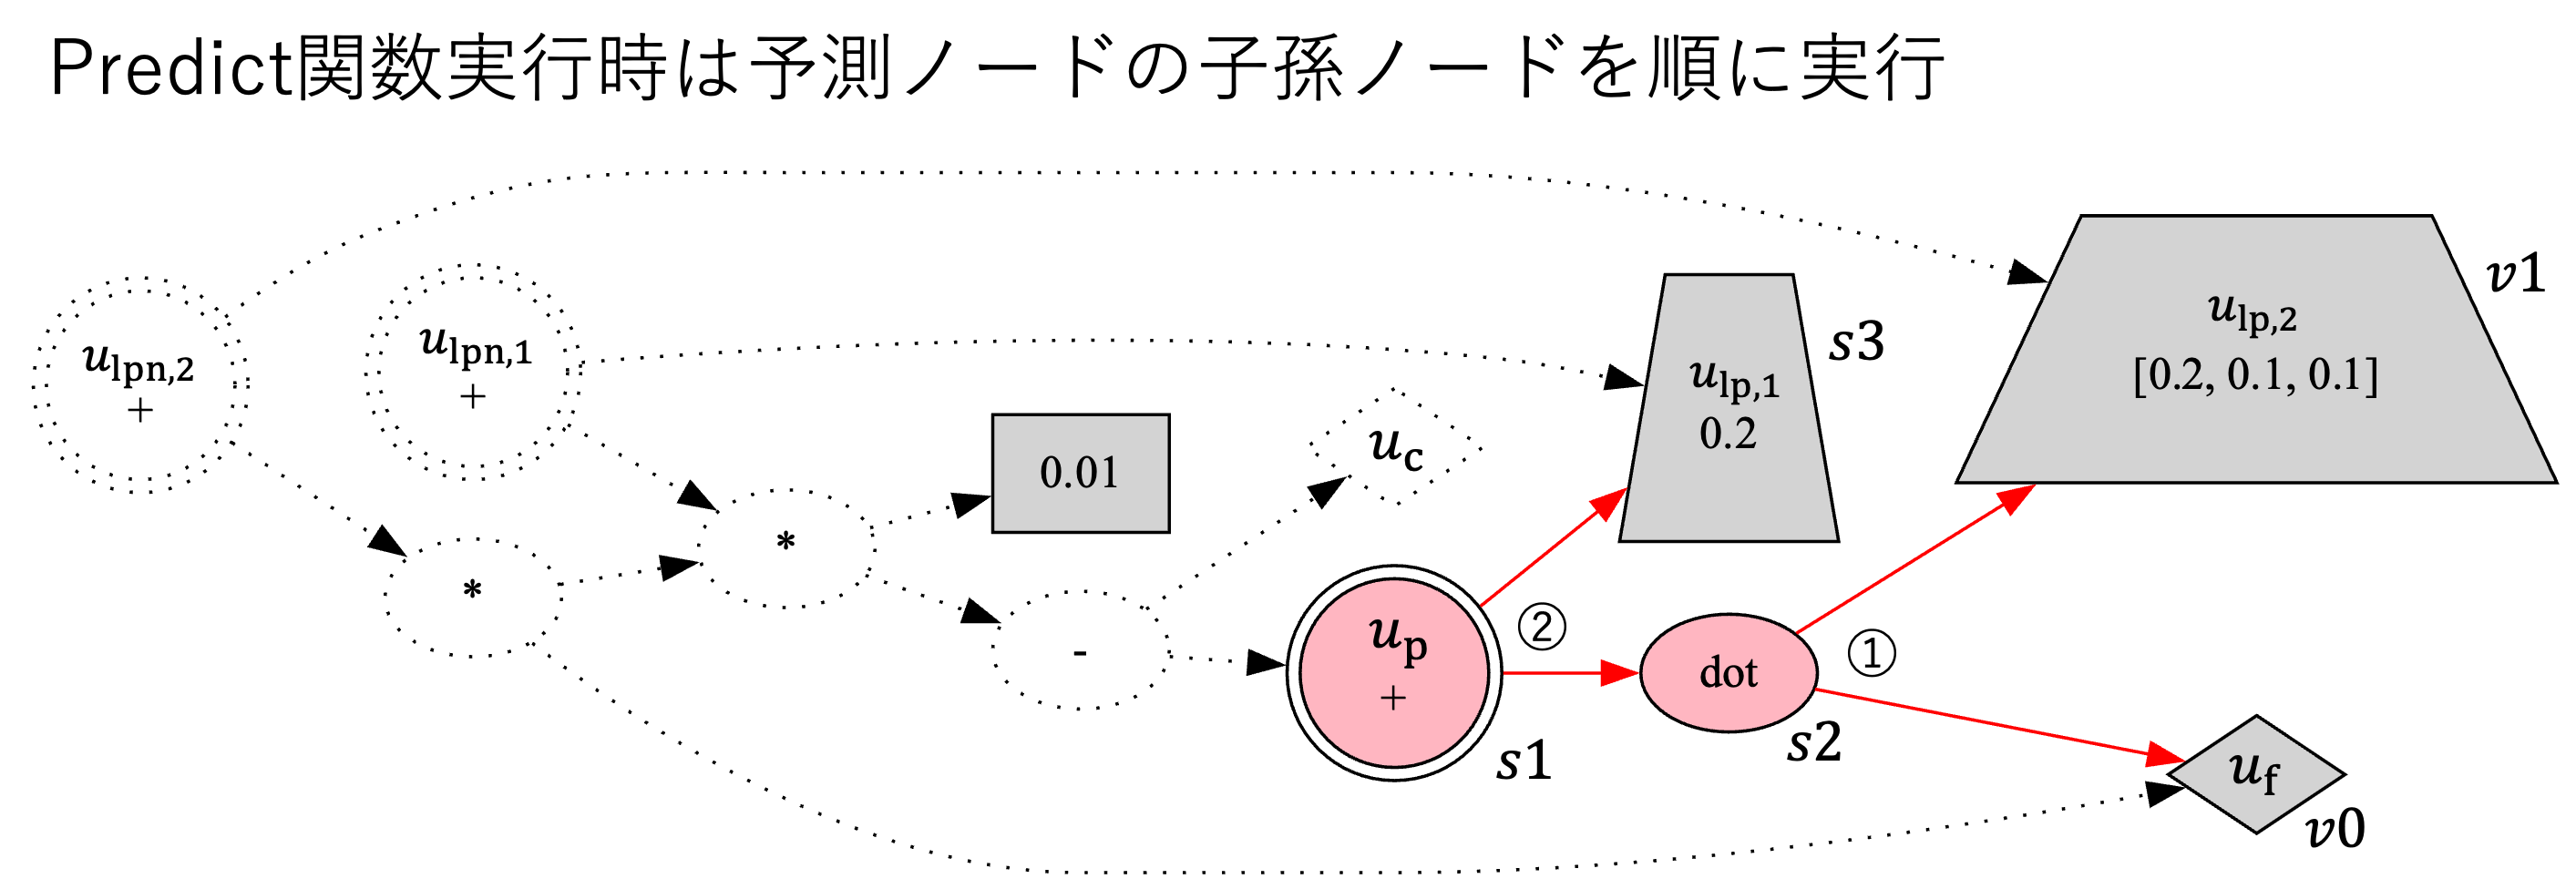
\includegraphics[width=14cm]{mgg_automl_zero_vag/ag/predict.png}
  \caption{予測時のAGの様子. 予測時は入力ベクトルノードに入力ベクトルが代入された後で, 着色したノードが処理される. まるで囲まれた数字はPredict関数における実行順を意味する. 予測ラベルノード$u_\mathrm{p}$の出力値が, 既存手法における予測ラベル$s1$の値として利用される.}
  \label{fig:mgg_automl_zero_vag:predict}
\end{figure}
\begin{figure}
  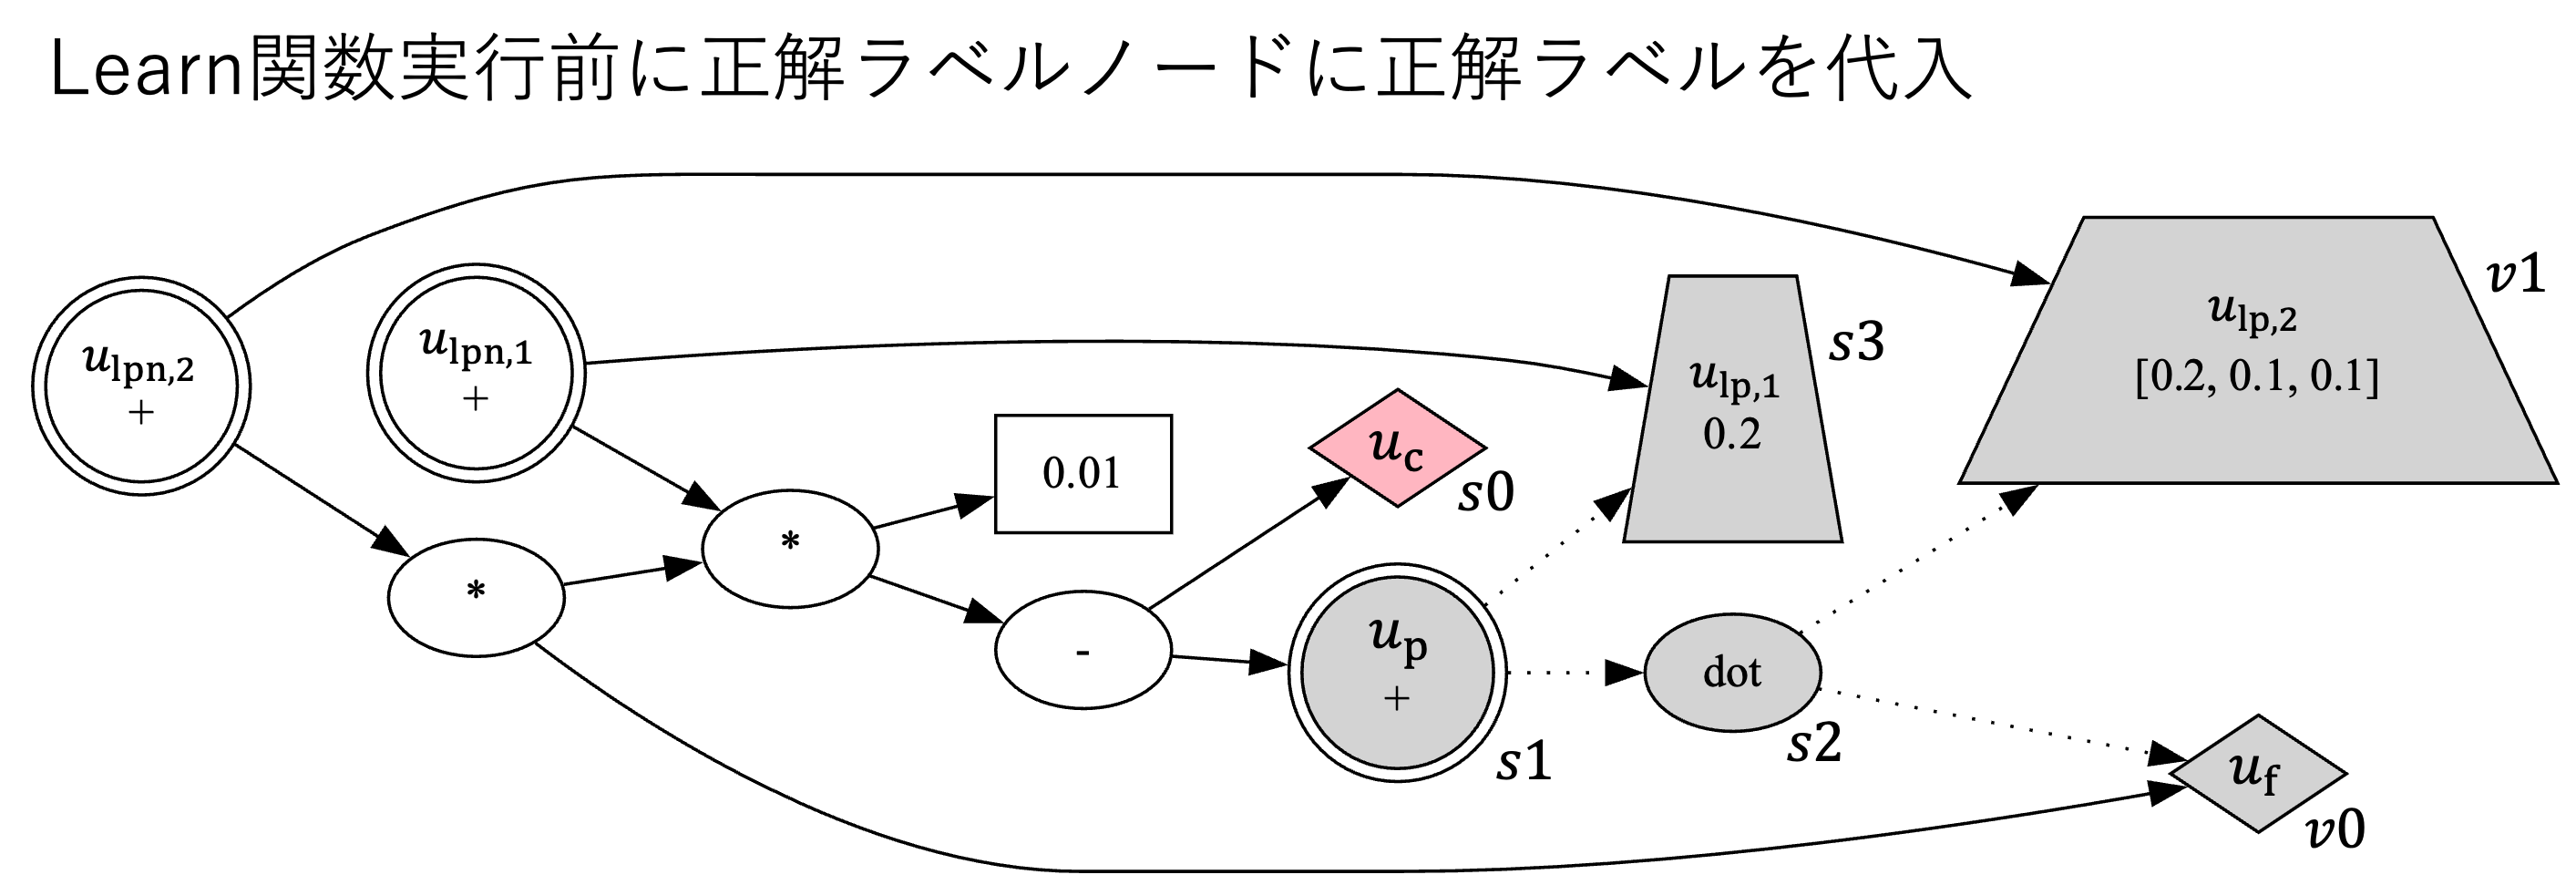
\includegraphics[width=14cm]{mgg_automl_zero_vag/ag/before_learn.png}
  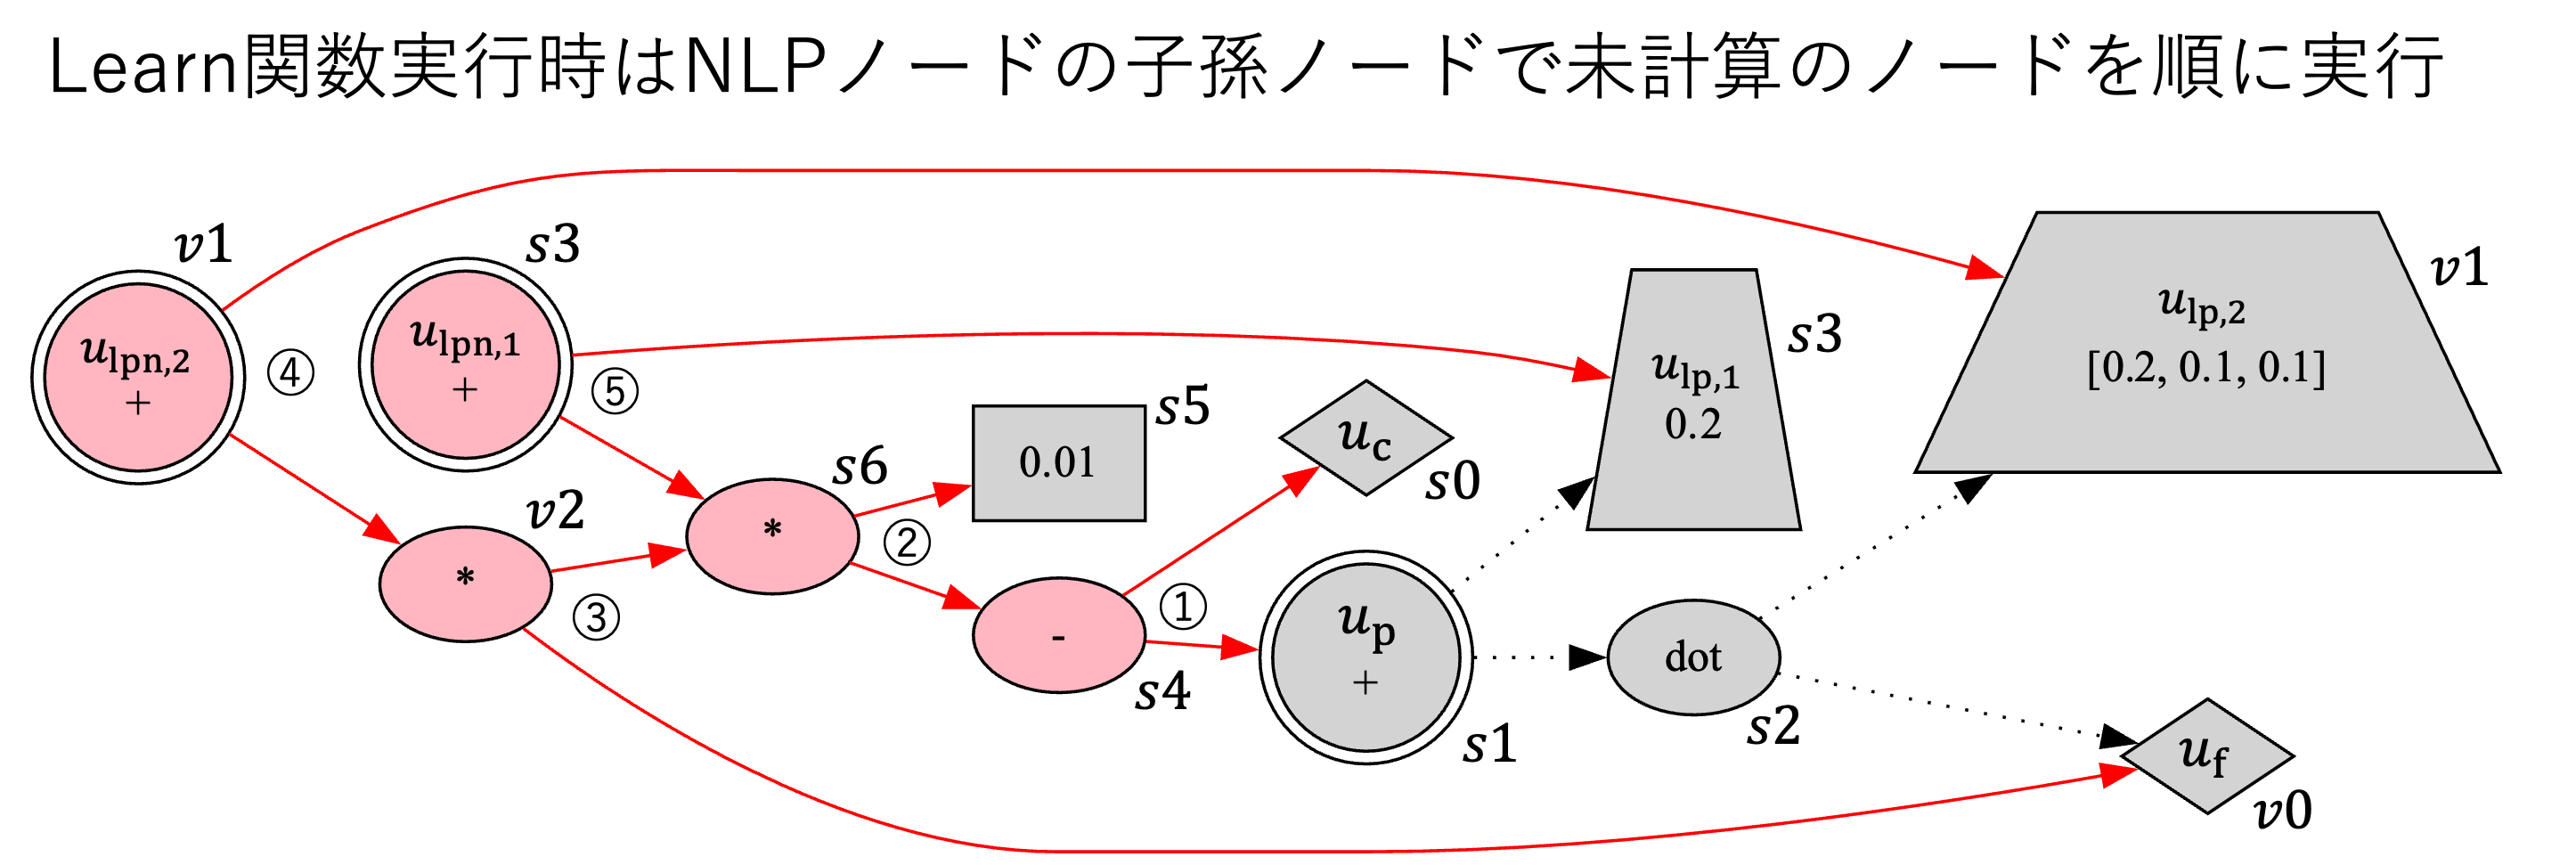
\includegraphics[width=14cm]{mgg_automl_zero_vag/ag/learn.png}
  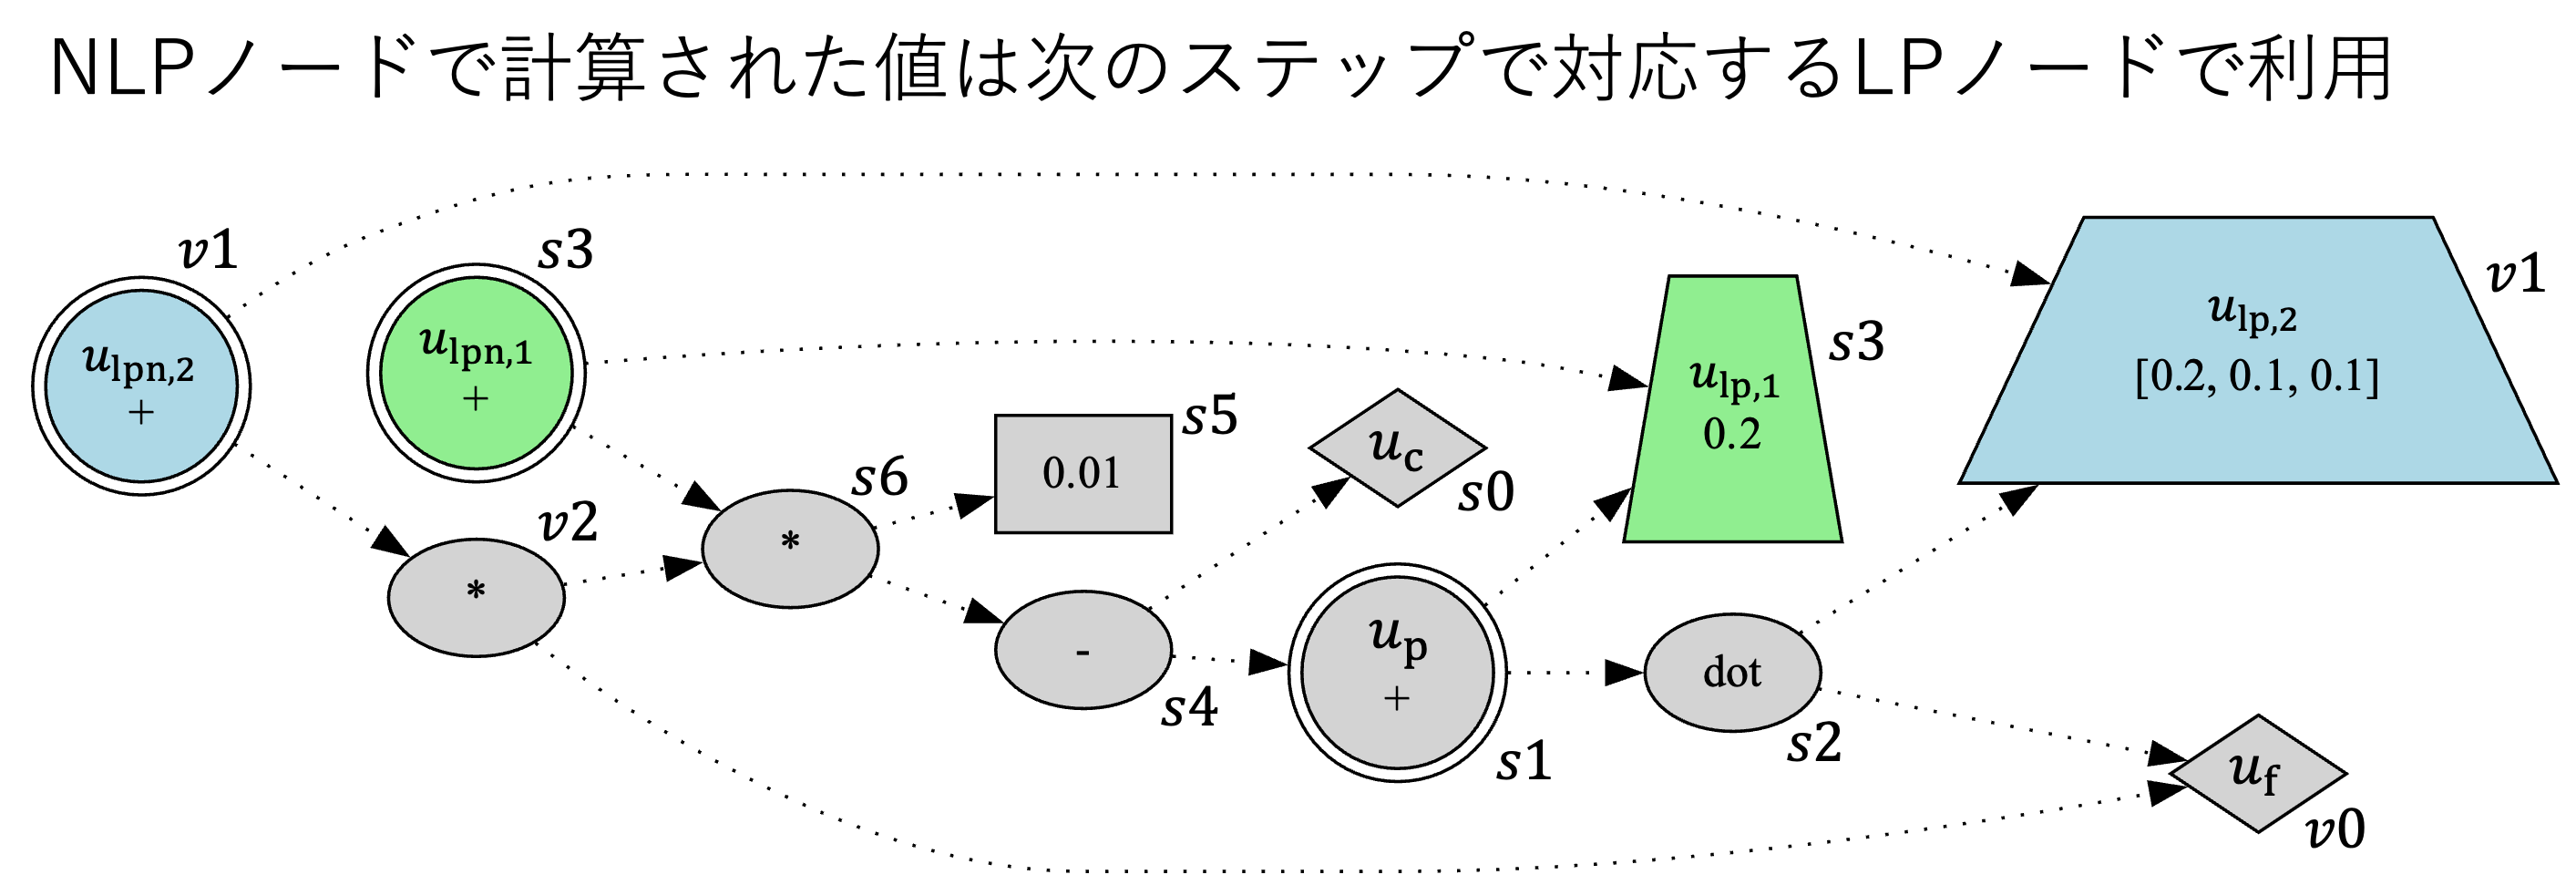
\includegraphics[width=14cm]{mgg_automl_zero_vag/ag/after_learn.png}
  \caption{学習時のAGの様子. 学習時は正解ラベルノードに正解ラベルが代入された後で, 着色したノードが処理される. まるで囲まれた数字はLearn関数における実行順を意味する. 各NLPノードの出力値は, 次のステップの対応するLPノードの値として利用される.}
  \label{fig:mgg_automl_zero_vag:learn}
\end{figure}

\subsection{AGによる冗長性の削減} \label{subsec:proposed:ag:redundancy}
本節では, AGによって削減可能な探索空間の冗長性について説明する. AGを導入することで, 既存手法の探索空間の冗長性の問題のうち, 変数名の違いによる冗長性と命令の実行順の違いによる冗長性に対処することができる. 既存手法では, 実行結果が同等で変数名のみが異なるアルゴリズムが区別されて扱われていた. 一方で, 提案手法のAGには変数名の情報は含まれていないため, 実行結果が同等で変数名のみが異なるアルゴリズムは同一視することができる. また, 既存手法では実行結果が同等で実行順序が異なるアルゴリズムがトポロジカルソートの数分だけ区別されて扱われてしまう. 一方で, 提案手法のAGでは依存関係のみを扱っており, 評価時にトポロジカルソートを1つ選んで実行するため, 実行結果が同等で実行順序が異なるアルゴリズムを同一視することができる.

非妥当なアルゴリズムに関する冗長性は, 依存関係が構造化されたAGに対して, 次節(第\ref{subsec:proposed:ag:vag}節)で述べる妥当なアルゴリズムの条件を規定し 条件を満たすAGのみを探索対象とすることで削減することができる.

\subsection{妥当なアルゴリズムグラフ (VAG)}\label{subsec:proposed:ag:vag}
本研究では, 以下の妥当なアルゴリズムの条件を満たすアルゴリズムグラフ$G = (U, E)$を, 妥当なアルゴリズムグラフ (Valid Algorithm Graph, VAG) と定義する.

\begin{enumerate}
  \item 全てのLPノード$u_{\mathrm{lp}, i} \in U$とNLPノード$u_{\mathrm{nlp}, i}\in U$に対して, 以下が満たされる.
  \begin{enumerate}
    \item $ u_{\mathrm{lp}, i}\in D_G(u_{\mathrm{nlp}, i})$
    \item $ u_{\mathrm{lp}, i} \in D_G(u_\mathrm{p}) \Rightarrow u_\mathrm{c} \in D_G(u_{\mathrm{nlp}, i}) $
    \item $ u_{\mathrm{lp}, i} \in D_G(u_\mathrm{c}) \Rightarrow u_\mathrm{c} \in D_G(u_{\mathrm{nlp}, i}) $
  \end{enumerate}
  \item $u_\mathrm{p} \in U$に関して以下が満たされる.
  \begin{enumerate}
    \item $v0 \in D_G(u_\mathrm{p})$
    \item $ \exists u_{\mathrm{lp}, i}, u_{\mathrm{lp}, i} \in D_G(u_\mathrm{p}) $
  \end{enumerate}
  \item 順序付き有向グラフ$G$が付録\ref{chap:ordered_directed_graph}に示した弱連結を持ち, 任意のノード$u \not\in D_G(u_\mathrm{p})$に対して, 以下の条件を満たすNLPノードの系列$ \pi: \{ 1,2,3,\cdots, m \}\rightarrow \{ i \in \mathbb{N} \ :\ 1 \leq i \leq N_\mathrm{lp}\} $が存在する. ここで, $N_\mathrm{lp}$はLPノードの総数である.
  \begin{itemize}
    \item $ u_{\mathrm{lp}, \pi(1)} \in D_G(u_\mathrm{p}) $
    \item $ u_{\mathrm{lp}, \pi(k+1)} \in D_G(u_{\mathrm{nlp}, \pi(k)}),\ k \in \mathbb{N},\ 1 \leq k \leq m - 1  $
    \item $ u \in D_G(u_{\mathrm{nlp}, \pi(m)}) \lor u = u_{\mathrm{nlp}, \pi(m)} $
  \end{itemize}
\end{enumerate}

\noindent
ここで, $D_G(u)$は$u$を始点として, 予測ノード$u_\mathrm{p}$を経由点として持たない経路で到達可能なノードの集合である. つまり, $u' \in U$であれば$u$を始点, $u'$を終点とする経路で, $u_\mathrm{p}$を経由点として持たない経路が存在する. 経路や経由点の詳細な定義は付録\ref{chap:ordered_directed_graph}を参照されたい. 本条件は, 第\ref{subsec:problem:existing_problem:space}節で述べた妥当なアルゴリズムの条件を, AGを用いて定式化したものである. 条件の番号は, 既存手法で述べた妥当なアルゴリズムの条件の番号と対応している.

\begin{figure}
  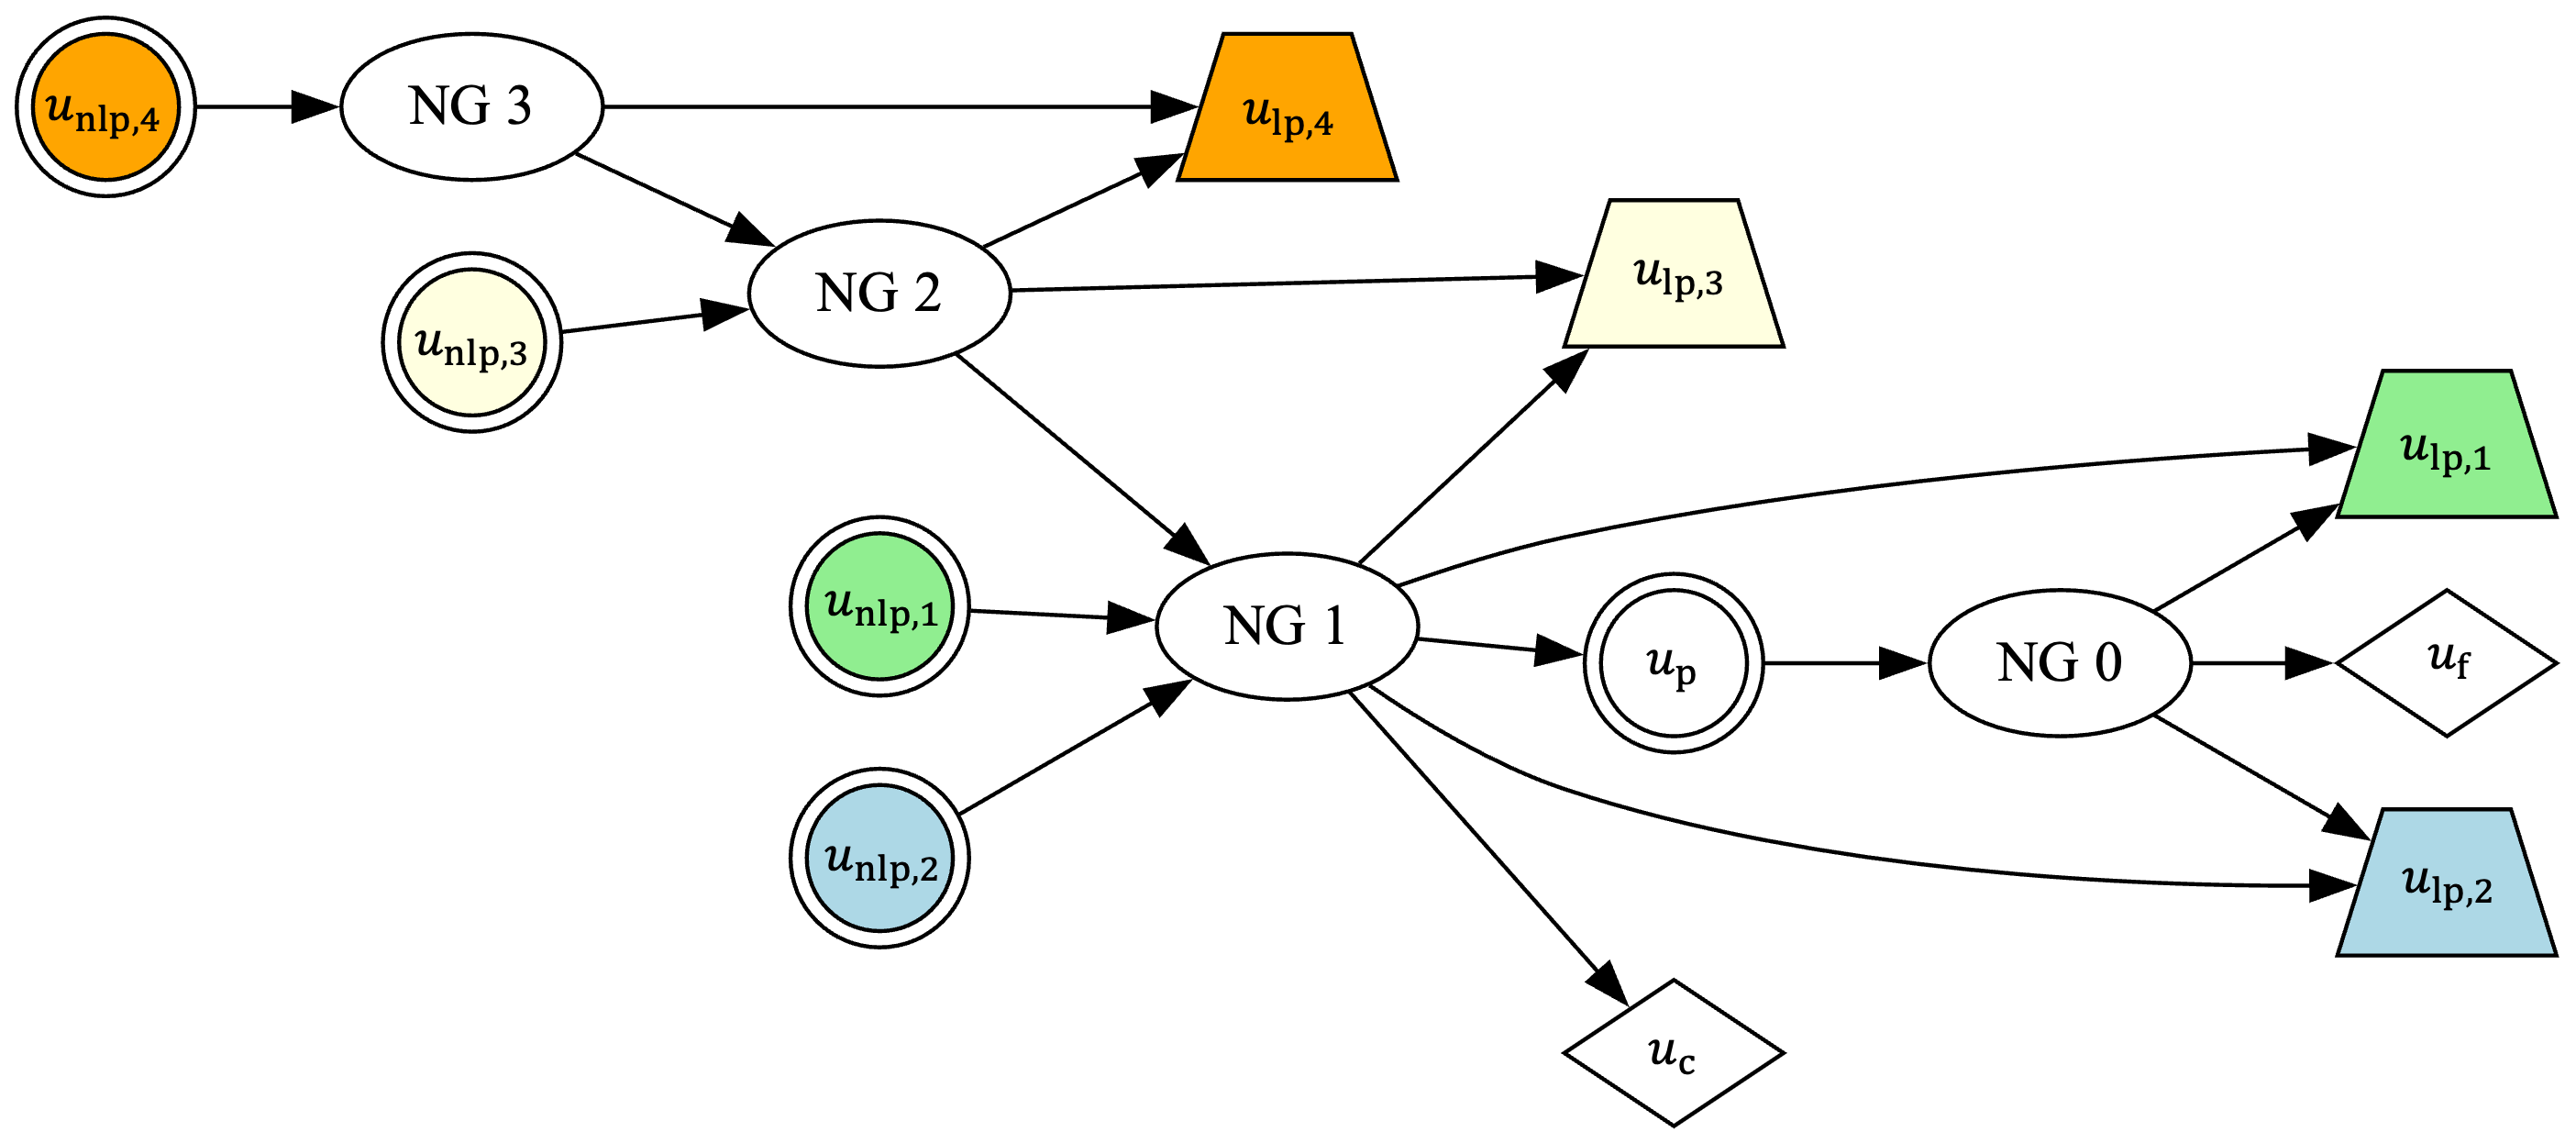
\includegraphics[width=14cm]{mgg_automl_zero_vag/ag/valid_lp.png}
  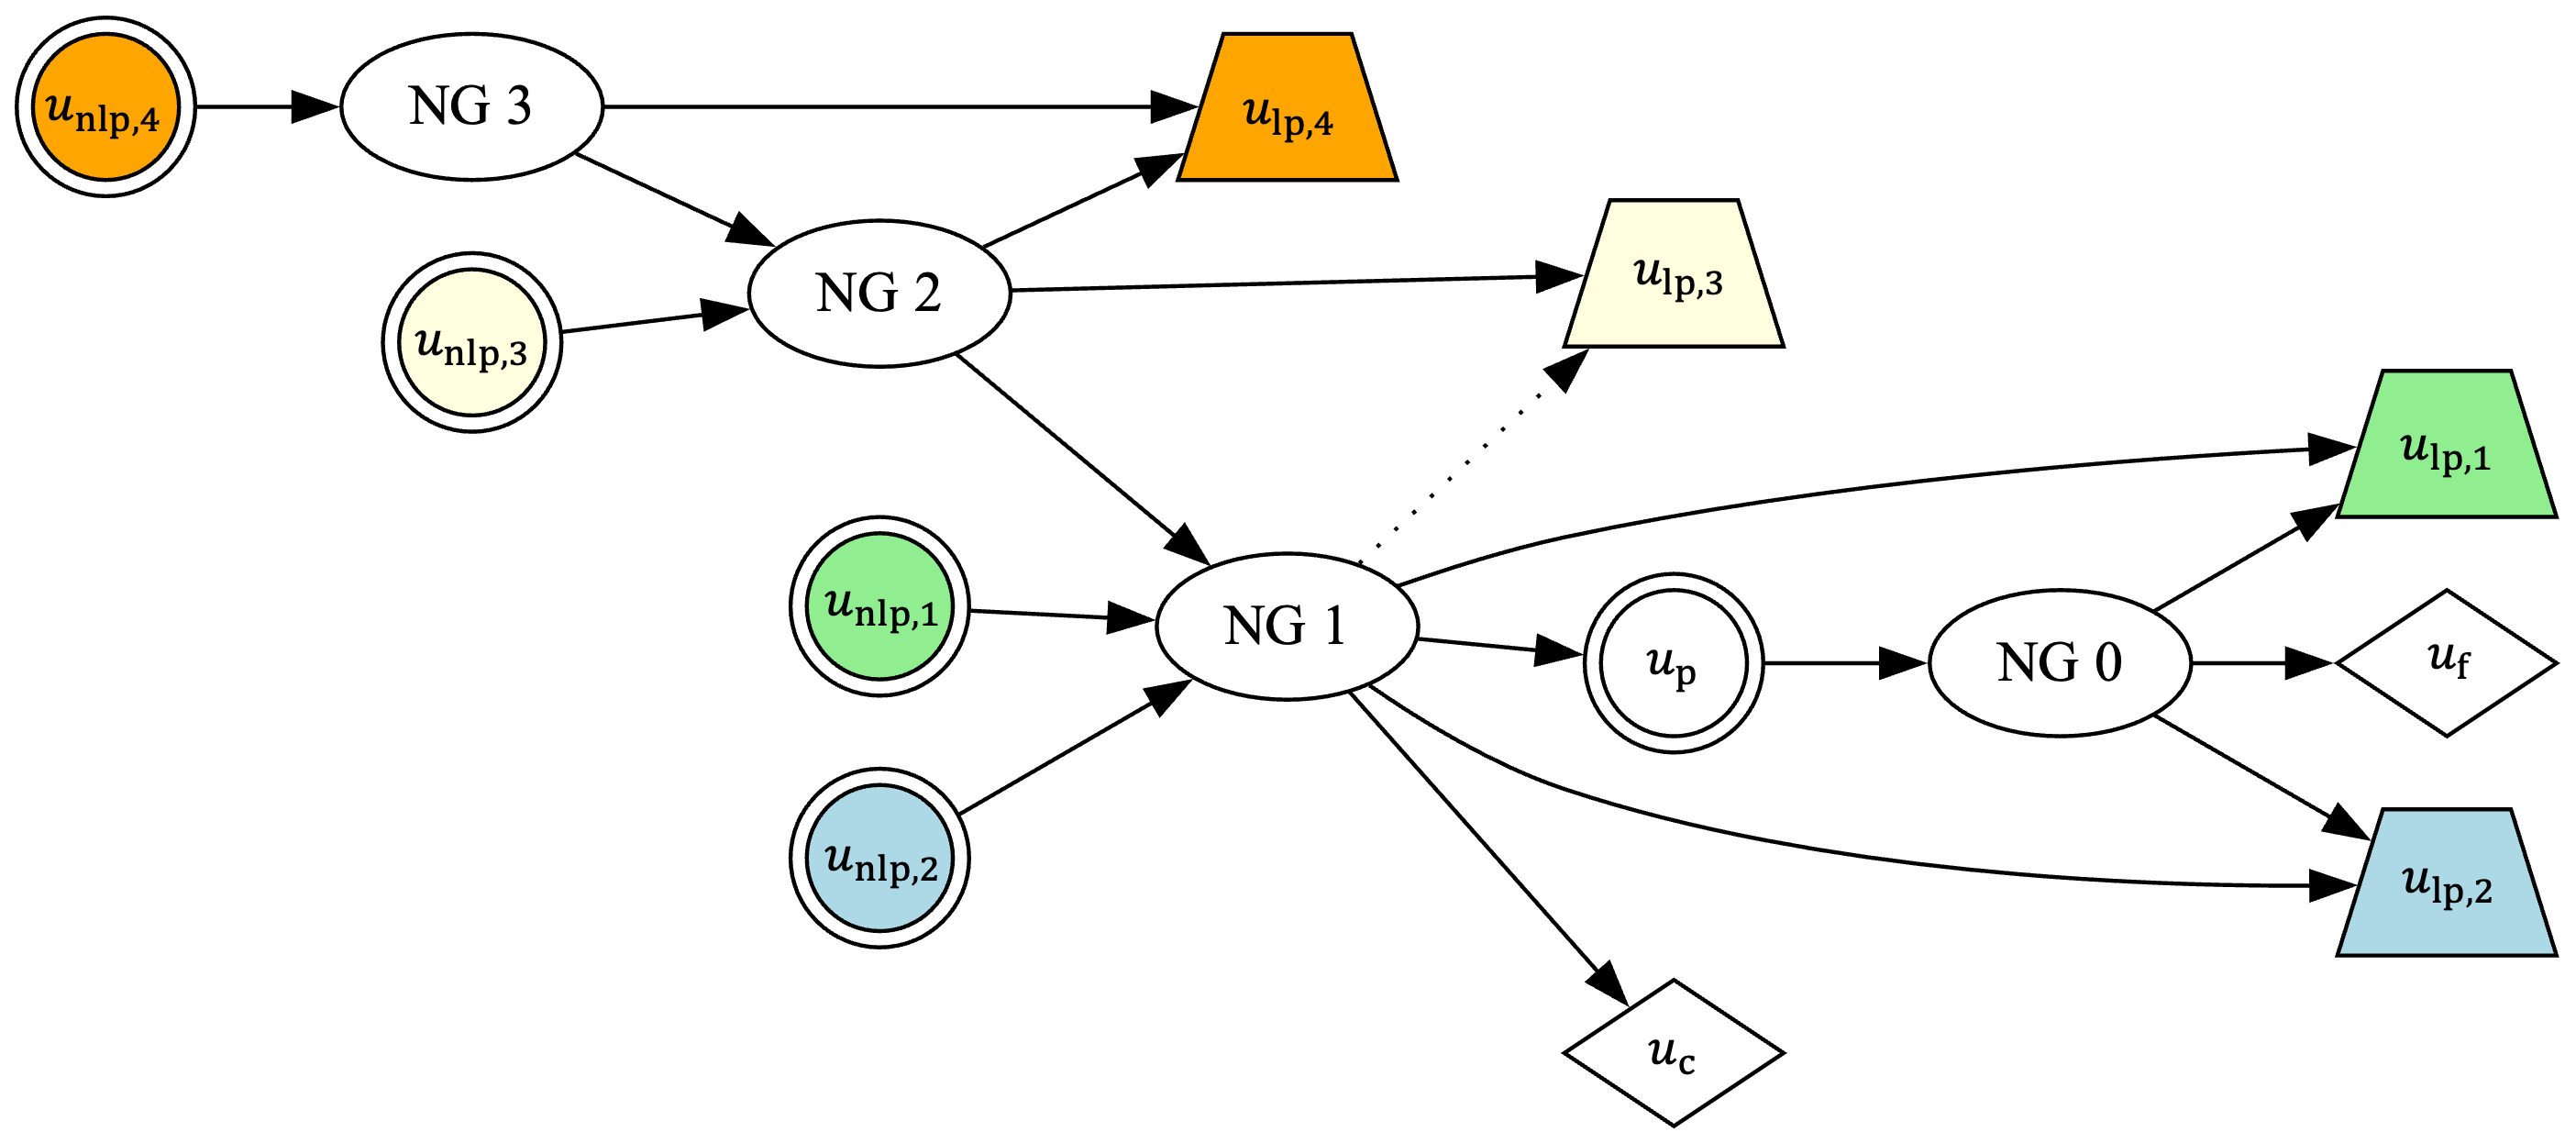
\includegraphics[width=14cm]{mgg_automl_zero_vag/ag/invalid_lp.png}
  \caption{妥当なアルゴリズムの条件3を満たすAG(上)と満たさないAG(下). 図においてNGは, ノードグループで複数のノードの集合である. 両者のAGの違いは, NG1から$u_{\mathrm{lp}, 3}$へのエッジが存在するかどうかのみで, その他は同等のAGである. 上のグラフでは, $\forall u \in \mathrm{NG3}$に対して, $\pi(1) = 2, \pi(2) = 3, \pi(3) = 4$とすれば, $u_{\mathrm{lp}, 2} \in D_G(u_\mathrm{p}),\ u_{\mathrm{lp}, 3} \in D_G(u_{\mathrm{nlp}, 2}),\ u_{\mathrm{lp}, 4} \in D_G(u_{\mathrm{nlp},3}),\ u \in D_G(u_{\mathrm{nlp}, 4})$を満たす. しかし, NG1から$u_{\mathrm{lp}, 3}$へのエッジが存在しない下のAGでは, $u_{\mathrm{nlp}, 2}$から$u_{\mathrm{lp}, 3}$への経路が存在しないため, $u_{\mathrm{lp}, 3} \not\in D_G(u_{\mathrm{nlp}, 2})$となり, NG3に含まれるノードに対して条件が満たされない..}
  \label{fig:mgg_automl_zero_vag:lp_validity}
\end{figure}


条件3については, 具体例を挙げて説明する. Fig.\ref{fig:mgg_automl_zero_vag:lp_validity}上に条件3を満たすAG, Fig.\ref{fig:mgg_automl_zero_vag:lp_validity}下に条件3を満たさないAGを示す. 図においてNGは, ノードグループで複数のノードの集合である. 上下の2つのグラフの違いは, NG1から$u_{\mathrm{lp}, 3}$へのエッジが存在するかどうかである. $u_{\mathrm{lp}, 3}$へのエッジが存在する上のAGでは条件3を満たす. 実際, $D_G(u_\mathrm{p})$に属さない各ノードに対して, 条件3を満たす系列$\pi$を構築ができる. 例えば, $\forall u \in \mathrm{NG3}$であれば, $\pi(1) = 2, \pi(2) = 3, \pi(3) = 4$とすれば, $u_{\mathrm{lp}, 2} \in D_G(u_\mathrm{p}),\ u_{\mathrm{lp}, 3} \in D_G(u_{\mathrm{nlp}, 2}),\ u_{\mathrm{lp}, 4} \in D_G(u_{\mathrm{nlp},3}),\ u \in D_G(u_{\mathrm{nlp}, 4})$を満たす. また, $u_{\mathrm{nlp}, 2}$であれば, $\pi(1) = 2$とすれば, $u_{\mathrm{lp}, 2} \in D_G(u_\mathrm{p}),\ u_{\mathrm{nlp}, \pi(1)} = u_{\mathrm{nlp}, 2}$を満たす. しかし, NG1から$u_{\mathrm{lp}, 3}$へのエッジが存在しないFig.\ref{fig:mgg_automl_zero_vag:lp_validity}下のAGでは, $u_{\mathrm{nlp}, 2}$から$u_{\mathrm{lp}, 3}$への経路が存在しないため, $u_{\mathrm{lp}, 3} \not\in D_G(u_{\mathrm{nlp}, 2})$となり, NG3に含まれるノードに対して条件が満たされない.

提案手法では, この妥当なアルゴリズムの条件を満たすVAGのみを探索することで, 既存手法の非妥当なアルゴリズムが探索対象となっている問題に対処する. VAGのみを探索対象とするために, 初期個体や突然変異による子個体の生成時にも, VAGのみが生成されるようにする必要がある. これらの詳細は, 第\ref{sec:proposed:initialization}節と第\ref{sec:proposed:mutation}節で述べる.

\subsection{VAGのノードのNLP媒介数}\label{subsec:proposed:ag:nlp_count}

VAGのノード$u \in U$におけるNLP媒介数$ C_\mathrm{nlp}(u) $を, 妥当なアルゴリズムの条件3を満たす最小の系列の長さと定義する. ただし, $u_\mathrm{p}$と$ D_G(u_\mathrm{p}) $内のノード$u$に対しては, $C_\mathrm{nlp}(u) = 0$と定義する 例えば, Fig.\ref{fig:mgg_automl_zero_vag:lp_validity}上のVAGでは, $\forall u \in \mathrm{NG3}$に対しては, $\pi(1) = 2, \pi(2) = 3, \pi(3) = 4$とすれば, $u_{\mathrm{lp}, 2} \in D_G(u_\mathrm{p}),\ u_{\mathrm{lp}, 3} \in D_G(u_{\mathrm{nlp}, 2}),\ u_{\mathrm{lp}, 4} \in D_G(u_{\mathrm{nlp},3}),\ u \in D_G(u_{\mathrm{nlp}, 4})$であり, 条件3を満たす最小の系列となるため, $C_\mathrm{nlp}(u) = 3$となる.

\subsection{AGの同一性と構造的同一性}\label{subsec:proposed:ag:equivalent}

本節では, AGに対する同一性と条件を弱めた構造的同一性について述べる. 2つのアルゴリズムが同一であるとは, 定数ノード, 入力ベクトルノード, 正解ラベルノード, LPノード, 命令ノード, 予測ノード, NLPノードを完全に保存する同型写像が存在することである. また, 構造的に同一であるとは定数ノードの値とLPノードの初期値のみが異なることを許容した同一性である. 本節では, それぞれの同一性について厳密に定義して, 具体例を挙げて説明する.

\subsubsection{同一性}

2つのアルゴリズムグラフ$G^A = (U^A, E^A)$, $G^B = (U^B, E^B)$が同一である ($G^A \equiv G^B$) とは, 以下の条件を満たす同型写像$ f: U_1 \rightarrow U_2 $が存在することと定義する.

\begin{enumerate}
  \item $f$が全単射である.
  \item $ \forall u_1, u_2 \in U^A, \forall n \in \mathbb{N} $に対して, $ (u_1, n, u_2) \in E^A \Leftrightarrow (f(u_1), n, f(u_2)) \in E^B $が成り立つ.
  \item $G^A$の入力ベクトルノードを$u_{\mathrm{f}}^A$, $G^B$の入力ベクトルノードを$u_{\mathrm{f}}^B$とすると, $f(u_{\mathrm{f}}^A) = u_{\mathrm{f}}^B$が成り立つ.
  \item $G^A$の正解ラベルノードを$u_\mathrm{c}^A$, $G^B$の正解ラベルノードを$u_\mathrm{c}^B$とすると, $f(u_\mathrm{c}^A) = u_\mathrm{c}^B$が成り立つ.
  \item $G^A$の予測ノードを$u_\mathrm{p}^A$, $G^B$の予測ノードを$u_\mathrm{p}^B$とすると, $f(u_\mathrm{p}^A) = u_\mathrm{p}^B$が成り立つ.
  \item $G^A$の任意の定数ノード$ u_\mathrm{const}^A \in U $に対して以下が成立する.
  \begin{enumerate}
    \item $f(u_\mathrm{const}^A)$は$G^B$の定数ノードである.
    \item $u_\mathrm{const}^A$と$f(u_\mathrm{const}^A)$に割り当てられている定数値が等しい.
  \end{enumerate}
  \item $G^A$の任意の命令ノード$u_\mathrm{op}^A \in U $に対して以下が成立する.
  \begin{enumerate}
    \item $f(u_\mathrm{op}^A)$は$G^B$の命令ノードである.
    \item $u_\mathrm{op}^A$と$f(u_\mathrm{op}^A)$に割り当てられている命令が等しい.
  \end{enumerate}
  \item $G^A$の任意のLPノード$u_\mathrm{lp}^A \in U $に対して以下が成立する.
  \begin{enumerate}
    \item $f(u_\mathrm{lp}^A)$は$G^B$のLPノードである.
    \item $u_\mathrm{lp}^A$と$f(u_\mathrm{lp}^A)$に割り当てられている学習パラメータの初期値が等しい.
  \end{enumerate}
  \item $G^A$の任意のNLPノード$u_\mathrm{nlp}^A \in U $に対して以下が成立する.
  \begin{enumerate}
    \item $f(u_\mathrm{nlp}^A)$は$G^B$のNLPノードである.
    \item NLPノード$u_\mathrm{nlp}^A$に対応するLPノードを$u_\mathrm{lp}^A$とすると, $G^B$においてNLPノード$f(u_\mathrm{nlp}^A)$に対応するLPノードは$f(u_\mathrm{lp}^A)$である.
  \end{enumerate}
\end{enumerate}

\noindent
AGが同一である関係はAG全体の集合$\mathcal{G}$上の同値関係となる. すなわち, AGの同一性は反射律, 対称律, 推移律を満たす. 実際, 反射律は恒等写像, 対称律は同型写像の逆写像, 推移律は二つの同型写像の合成写像を考えることで容易に示される.

\subsubsection{構造的同一性}
AGの同一性から定数ノードの値と学習パラメータの初期値の同一条件を外した構造的同一性を定義する. 2つのアルゴリズムグラフ$G^A = (U^A, E^A)$, $G^B = (U^B, E^B)$が構造的に同一である ($G^A \equiv_\mathrm{struct} G^B$) とは, 同型写像の条件のうち6 (b)と8 (b)を除いた条件を満たす写像$ f: U_1 \rightarrow U_2 $が存在することと定義する. 構造的同一性の関係も同一性の関係と同様に, $\mathcal{G}$上の同値関係となる.

構造的同一性に関して, 具体例を挙げて説明する. Fig.\ref{fig:mgg_automl_zero_vag:eq1}に, Fig.\ref{fig:mgg_automl_zero_vag:affine}のAGと構造的同一のAGを示す. 2つのAGの違いは, 定数ノードの値, LPノードの初期値のみである. また, Fig.\ref{fig:mgg_automl_zero_vag:neq1}と\ref{fig:mgg_automl_zero_vag:neq2}に, Fig.\ref{fig:mgg_automl_zero_vag:affine}のAGと構造的同一性を持たないAGを示す. Fig.\ref{fig:mgg_automl_zero_vag:neq1}のAGは命令ノードに割り当てられている命令が異なり, Fig.\ref{fig:mgg_automl_zero_vag:neq2}のAGは命令ノードに割り当てられている子ノードの順序が異なる.

\begin{figure}
  \centering
  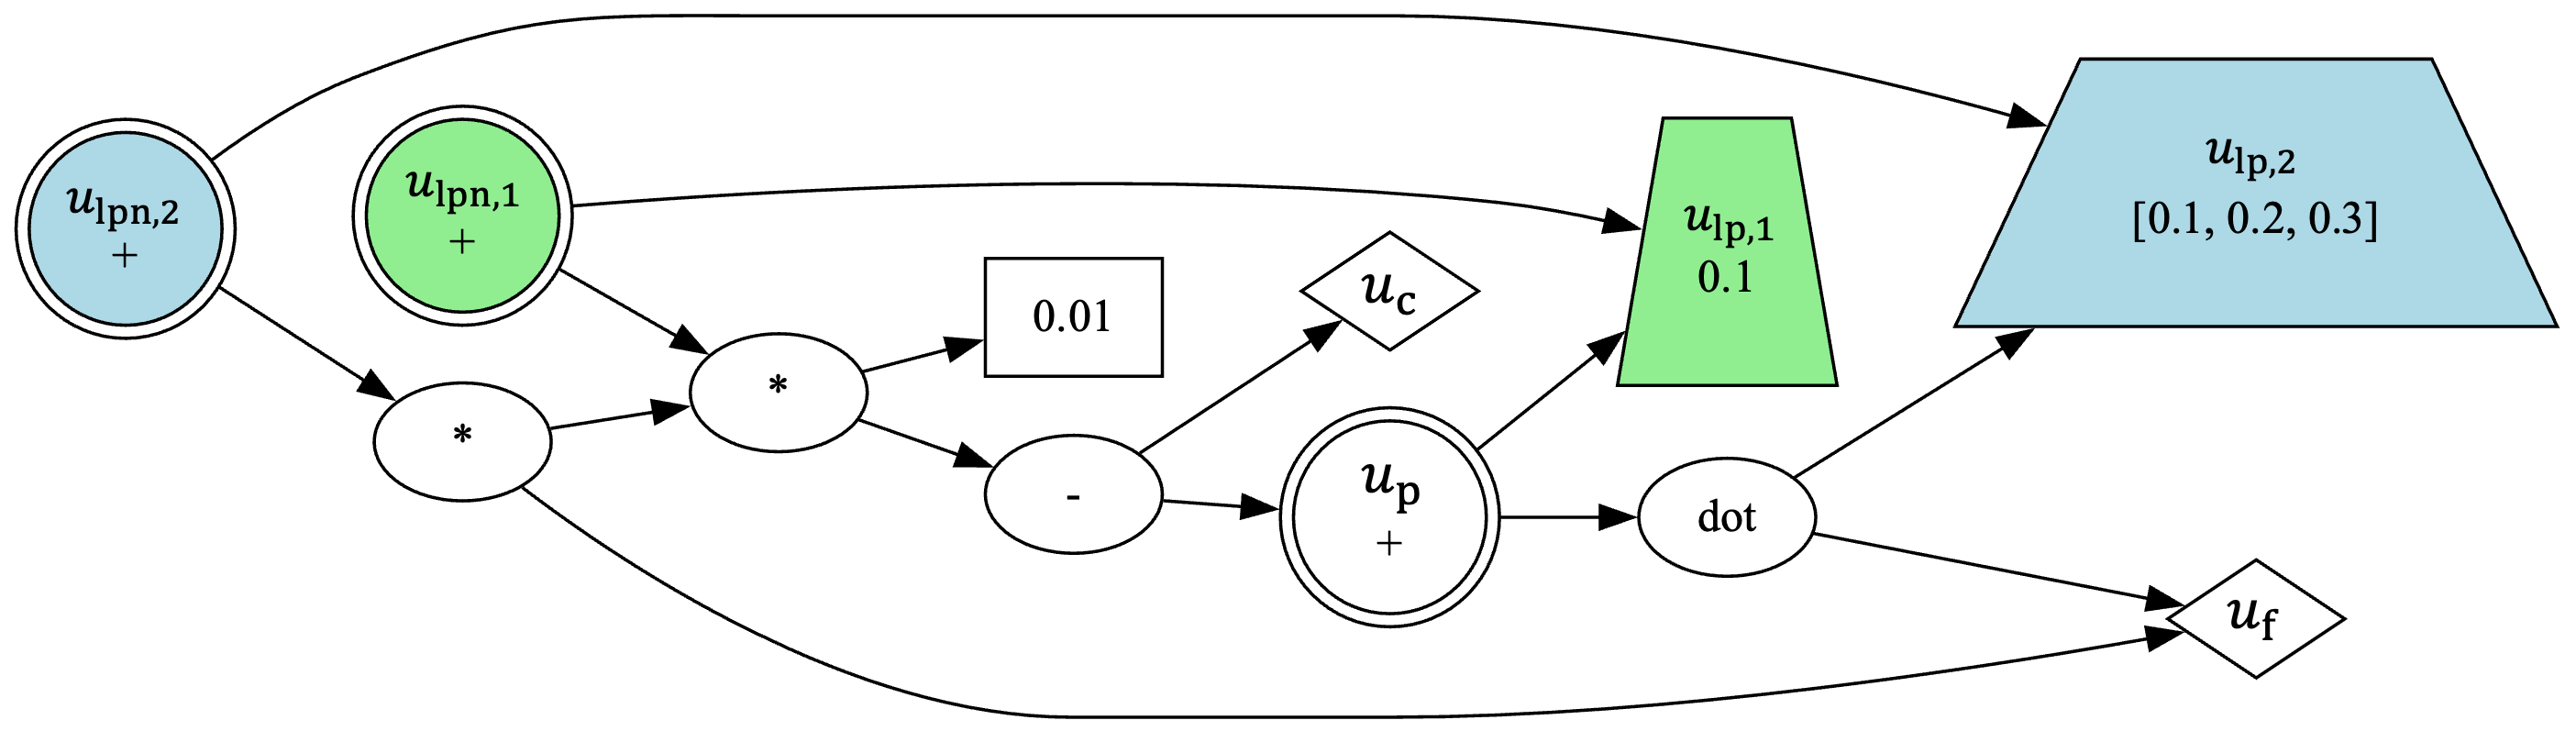
\includegraphics[width=14cm]{mgg_automl_zero_vag/ag/eq.png}
  \caption{Fig.\ref{fig:mgg_automl_zero_vag:affine}のAGと構造的同一のAG. 2つのAGの違いは, 定数ノードの値, LPノードの初期値のみである}
  \label{fig:mgg_automl_zero_vag:eq1}
\end{figure}

\begin{figure}
  \centering
  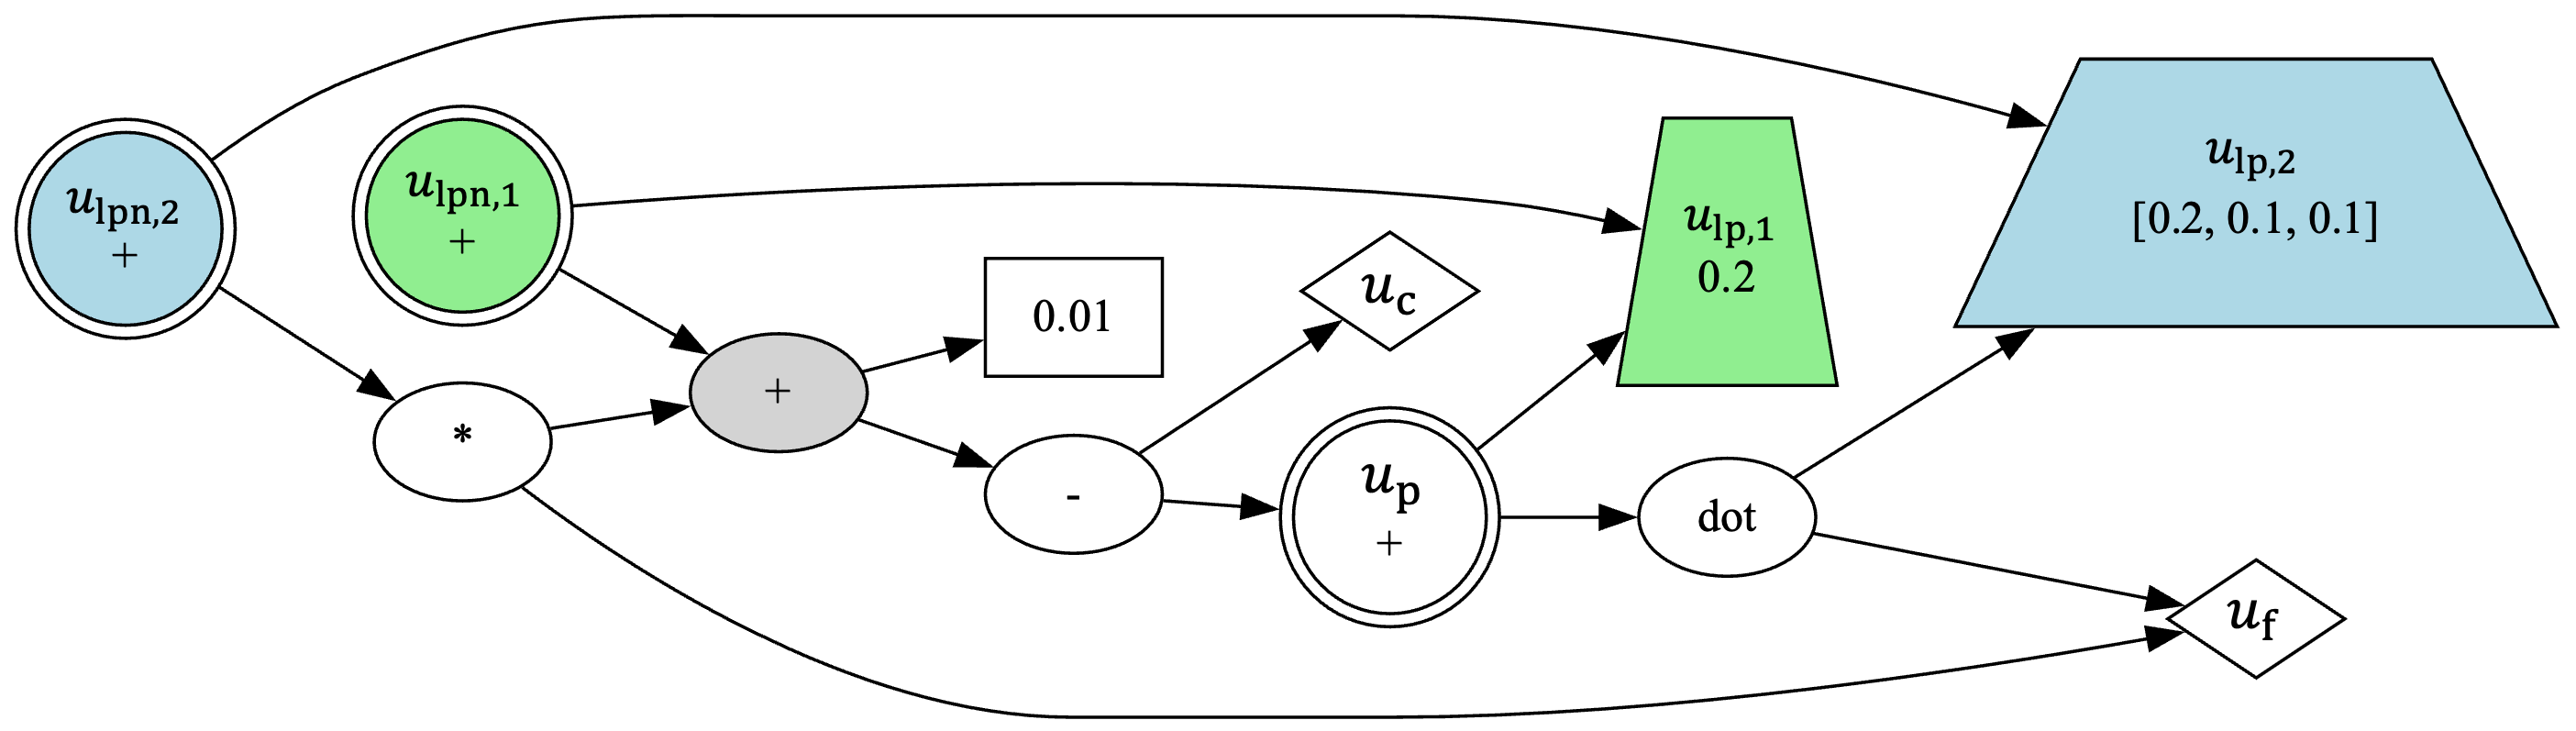
\includegraphics[width=14cm]{mgg_automl_zero_vag/ag/neq1.png}
  \caption{Fig.\ref{fig:mgg_automl_zero_vag:affine}のAGと構造的同一ではないAG. 灰色で着色された命令ノードに割り当てられている命令が異なる.}
  \label{fig:mgg_automl_zero_vag:neq1}
\end{figure}

\begin{figure}
  \centering
  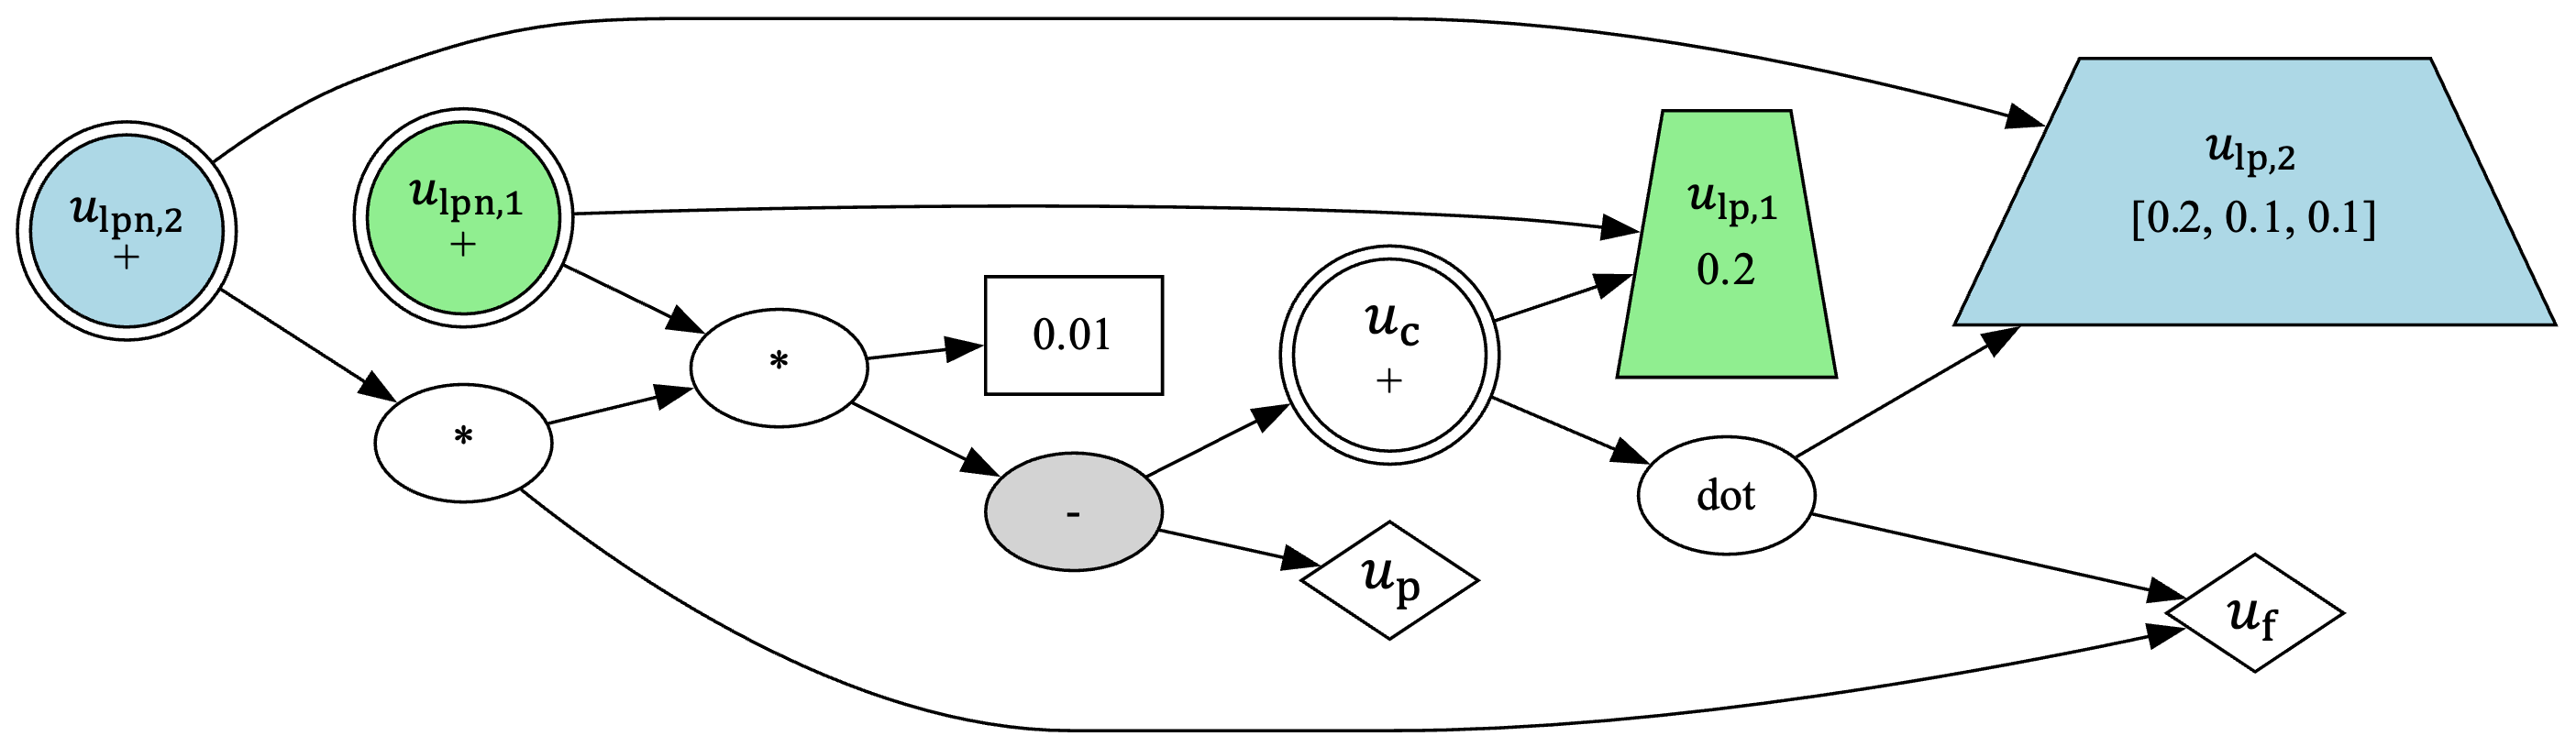
\includegraphics[width=14cm]{mgg_automl_zero_vag/ag/neq2.png}
  \caption{Fig.\ref{fig:mgg_automl_zero_vag:affine}のAGと構造的同一ではないAG. 灰色で命令ノードに割り当てられている子ノードの順序が異なる.}
  \label{fig:mgg_automl_zero_vag:neq2}
\end{figure}

\section{初期個体の生成}\label{sec:proposed:initialization}

提案手法では, VAGのみを探索対象とするために, 予測ノード$u_\mathrm{p}$を起点として, 妥当なアルゴリズムの条件を反映させながら, グラフを段階的に構築していくことでVAGの生成を行う. 具体的には, 予測ノード$u_\mathrm{p}$と$D_G(u_\mathrm{p})$を構築した後で, ノードのNLP媒介数が小さい順でNLPノード$u_{\mathrm{nlp},i}$と$D_G(u_{\mathrm{nlp},i})$を構築する. ここで, $D_G(u)$は$u$を始点として, 予測ノード$u_\mathrm{p}$を経由点として持たない経路で到達可能なノードの集合である. つまり, $u' \in U$であれば$u$を始点, $u'$を終点とする経路で, $u_\mathrm{p}$を経由点として持たない経路が存在する. 経路や経由点の詳細な定義は付録\ref{chap:ordered_directed_graph}を参照されたい.

本節では, 第\ref{subsec:proposed:initialization:basic_operation}節で初期個体を生成するために必要なノードの基本操作について説明した後で, 第\ref{subsec:proposed:initialization:s1}節で$u_\mathrm{p}$と$D_G(u_\mathrm{p})$を構築する方法, 第\ref{subsec:proposed:initialization:nlp}節でNLPノード$u_{\mathrm{nlp},i}$と$D_G(u_{\mathrm{nlp},i})$を構築する方法について説明する.

\subsection{ノードの基本操作} \label{subsec:proposed:initialization:basic_operation}

アルゴリズムグラフ$G=(U, E)$において, ノード$u$と$D_G(u)$の構築をするために必要な基本操作を以下に示す. 以下の操作の説明において, ノード$u \in U$の配下の未使用入力の集合$A(u)$を以下のように定義する:
$$
A(u) = \{ (u_\mathrm{op}, n) \in U \times \mathbb{N} \ :\ u_\mathrm{op} \in u \cup D_G(u),\ n \in N_\mathrm{in}(u_\mathrm{op}),\ \not\exists u' \in U,\ (u_\mathrm{op}, n, u') \in E \}
$$
\noindent
ここで, $N_\mathrm{in}(u_\mathrm{op})$は命令ノード$u_\mathrm{op}$の命令の入力の数を表す. $A(u)$は$u \cup D_G(u)$内の命令ノードのうち, 入力(子ノード)に空きがあるノードとその順序値の組みを集めた集合である. また, $A(u) \neq \emptyset$である時, 命令ノード$u$配下には未使用の入力が存在すると表現する.

\subsubsection{命令ノード構築操作 (add\_op\_node)}

命令ノード構築操作は, 指定された型$\mathrm{type}$を出力の型とする命令ノード$u_\mathrm{op}$を作成して, $G$に追加する操作$U \leftarrow U \cup \{ u_\mathrm{op} \}$である. 入力は, アルゴリズムグラフ$G$, 作成する命令ノードの型$\mathrm{type}$, 命令セット$\mathrm{OP}$で, 出力は構築された命令ノード$u_\mathrm{op}$である.

\subsubsection{命令ノード拡張操作 (extend\_op\_node)}
命令ノード拡張操作は, ノード$u$配下の未使用入力$(u_\mathrm{op},n) \in A(u)$を一様ランダムに選択して, 型が整合的な命令ノード$u_\mathrm{op}'$を構築して割り当てる操作$G \leftarrow G \cup \{ u_\mathrm{op}' \},\ E \leftarrow E \cup \{ (u_\mathrm{op}, n, u_\mathrm{op}') \} $である. 命令ノード$u_\mathrm{op}'$は, 命令ノード構築操作によって初期化される. 入力は, アルゴリズムグラフ$G$, 命令ノード拡張操作の対象ノード$u$, 命令セット$\mathrm{OP}$であり, 出力は拡張して構築された命令ノードである.

\subsubsection{接続操作 (connect\_node)}
接続操作は, ノード$u$配下のそれぞれの未使用入力$(u_\mathrm{op},n) \in A(u)$に対して, $u_\mathrm{op}$の第$n$引数と型が整合的な$u' \in U$を一様ランダムに選択し, 一定確率$p_\mathrm{conn}$で割り当てる操作$E \leftarrow E \cup \{ (u_\mathrm{op}, n, u') \} $である. 入力は, アルゴリズムグラフ$G$, 接続操作の対象ノード$u$, 接続確率$p_\mathrm{conn}$であり, 出力は存在しない.

\subsubsection{ノード指定接続操作 (connect\_specifed\_node)}
ノード指定接続操作は, ノード$u$の配下の未使用入力$(u_\mathrm{op},n) \in A(u)$を一様ランダムに選択して, 指定されたノード$u_0$を割り当てる操作$E \leftarrow E \cup \{ (u_\mathrm{op}, n, u_0) \} $である. ただし, $u_\mathrm{op}$の第$n$引数と型と指定されたノード$u_0$の型は整合的である必要がある. 入力は, アルゴリズムグラフ$G$, ノード指定接続操作の対象ノード$u$, 接続するノード$u_0$であり, 出力は存在しない.

\subsubsection{LPノード構築操作 (add\_lp\_node)}
LPノード構築操作は, $\{v\} \cup D_G(v)$に含まれる命令ノードのうち, 入力(子ノード)に空きがあるノードを一様ランダムに1つ選択し, 選択されたノードの入力と整合的な型を持つLPノードを初期化して割り当てる操作である. ここで, LPノードを初期化する際には, 学習パラメータの初期値は標準正規分布に従ってランダムに初期化される. 構築されたノードは, アルゴリズムグラフ$G$に追加される. 入力は, アルゴリズムグラフ$G$, LPノード構築操作の対象となるノード$v$であり, 出力は構築したLPノードである.

\subsubsection{終端接続操作 (connect\_terminal\_nodes)}
終端接続操作は, ノード$u$配下のそれぞれの未使用入力$(u_\mathrm{op},n) \in A(u)$に対して, $u_\mathrm{op}$の第$n$引数と型が整合的な終端ノード$u_\mathrm{term} \in U$を一様ランダムに選択し, 一定確率$\hat{p}_\mathrm{conn}$で割り当てる操作$E \leftarrow E \cup \{ (u_\mathrm{op}, n, u_\mathrm{term}) \} $である. 入力は, アルゴリズムグラフ$G$, 終端接続操作の対象となるノード$v$, 接続確率$\hat{p}_\mathrm{conn}$であり, 出力は存在しない

\subsubsection{定数割当操作 (add\_const\_nodes)}
定数割当操作は, ノード$u$配下のそれぞれの未使用入力$(u_\mathrm{op},n) \in A(u)$に対して, 定数ノード$u_\mathrm{const}$を初期化して割り当てる操作$U \leftarrow U \cup \{u_\mathrm{const}\},\ E \leftarrow E \cup \{ (u_\mathrm{op}, n, u_\mathrm{const}) \} $である. ここで, 各定数ノード$u_\mathrm{const}$を初期化する際には, スカラー型の場合は標準正規分布に従ってランダムに初期化され, ベクトル型や行列型の場合は各要素が標準正規分布に従ってランダムに初期化される. 入力は, アルゴリズムグラフ$G$, 定数割当操作の対象となるノード$v$であり, 出力は存在しない.

\subsection{$u_\mathrm{p}$と$D_G(u_\mathrm{p})$の構築} \label{subsec:proposed:initialization:s1}

$u_\mathrm{p}$と$D_G(u_\mathrm{p})$の構築方法をAlgorithm \ref{algorithm:construct_s1_node}に示す. 予測ノード$u_\mathrm{p}$と$D_G(u_\mathrm{p})$の構築では, 命令数$N_{\mathrm{OP}}^{(0)}$, 学習パラメータの最大数$N_{\mathrm{LP}, \mathrm{max}}^{(0)}$, 接続確率$p^{(0)}_\mathrm{conn}$, 終端接続確率$\hat{p}^{(0)}_\mathrm{conn}$を入力として受け取り, NLP媒介数0まで構築済みのアルゴリズムグラフ$G^{(0)}$, NLP媒介数0の学習パラメータの集合$S_\mathrm{LP}^{(0)}$を出力する. 詳細なアルゴリズムの説明を以下に示す.

\begin{breakablealgorithm}
  \caption{$u_\mathrm{p}$と$D_G(u_\mathrm{p})$の構築}
  \label{algorithm:construct_s1_node}
  \begin{algorithmic}[1]
    \REQUIRE \ \\
    \begin{itemize}
      \item 命令セット$\mathrm{OP}^{(0)}$
      \item 命令数$N_{\mathrm{OP}}^{(0)}$
      \item 学習パラメータの数$N_{\mathrm{LP}}^{(0)}$
      \item 接続確率$p^{(0)}_\mathrm{conn}$
      \item 終端接続確率$\hat{p}^{(0)}_\mathrm{conn}$
    \end{itemize}
    \ENSURE \ \\
    \begin{itemize}
      \item NLP媒介数$0$まで構築済みのアルゴリズムグラフ$G^{(0)}$
      \item NLP媒介数$0$のLPノードの集合$S_\mathrm{LP}^{(0)}$
    \end{itemize}
    \STATE $ V_G \leftarrow \{ u_\mathrm{f} \} $
    \STATE $ E_G \leftarrow \emptyset $
    \STATE $ G^{(0)} \leftarrow (V_G, E_G) $
    \STATE $ S_\mathrm{LP}^{(0)} \leftarrow \emptyset  $
    \STATE $ u_\mathrm{p} \leftarrow \mathrm{add\_op\_node}(G, \mathrm{SCALAR}, \mathrm{OP}^{(0)}) $
    \STATE $ \mathrm{connect\_node}(G, u_\mathrm{p}, p^{(0)}_\mathrm{conn}, \mathrm{OP}) $
    \FOR{$i \leftarrow 2$ to $N_{\mathrm{OP}}^{(0)}$}
    \STATE $ u_\mathrm{op} \leftarrow \mathrm{extend\_op\_node}(G, u_\mathrm{p}, \mathrm{OP}^{(0)}) $
    \STATE $ \mathrm{connect\_node}(G, u_\mathrm{op}, p^{(0)}_\mathrm{conn}, \mathrm{OP}^{(0)}) $
    \ENDFOR
    \IF{$ u_\mathrm{f} \not\in D_G(u_\mathrm{p})$}
    \STATE $ \mathrm{connect\_specified\_node}(G, u_\mathrm{p}, u_\mathrm{f}) $
    \ENDIF
    \FOR{$i \leftarrow 1$ to $N_{\mathrm{LP}}^{(0)}$}
    \STATE $ u_\mathrm{lp} \leftarrow \mathrm{add\_lp\_node}(G, u_\mathrm{p}) $
    \STATE $ S_\mathrm{LP}^{(0)} \leftarrow S_\mathrm{LP}^{(0)} \cup \{ u_\mathrm{lp} \} $
    \ENDFOR
    \STATE $ \mathrm{connect\_terminal\_nodes}(G, u_\mathrm{p}, \hat{p}^{(0)}_\mathrm{conn}) $
    \STATE $ \mathrm{add\_const\_nodes}(G, u_\mathrm{p}) $
    \RETURN $G^{(0)}$, $S_\mathrm{LP}^{(0)}$
  \end{algorithmic}
\end{breakablealgorithm}

以下に, Algorithm \ref{algorithm:construct_s1_node}の詳細な説明を示す.

\begin{description}
  \item[1行目] アルゴリズムグラフのノードの集合に$u_\mathrm{f}$を入れて初期化する.
  \item[2行目] アルゴリズムグラフのエッジの集合には何も追加せずに初期化する.
  \item[3行目] ノードとエッジからアルゴリズムグラフを初期化する.
  \item[4行目] NLP媒介数が0のLPノードの集合を空集合で初期化する.
  \item[5行目] 命令ノード構築操作によって$u_\mathrm{p}$ノードを構築する.
  \item[6行目] 作成された$u_\mathrm{p}$ノードに対して接続操作を適用する.
  \item[7-10行目] 所与の命令数になるまで命令ノード拡張操作と接続操作を繰り返す.
  \item[11-13行目] 予測ラベル$u_\mathrm{p}$に$u_\mathrm{f}$が使われていない場合は, ノード指定接続操作で$u_\mathrm{f}$を接続する.
  \item[14-17行目] $N_\mathrm{LP}^{(0)}$個の学習パラメータをLPノード構築操作で終端ノードに追加する.
  \item[18行目] 終端接続操作によって, 空きがあるノードを一定確率で既存の終端ノードと接続する.
  \item[19行目] 終端接続操作を適用後にも埋まらなかったノードを定数割当操作によって, 定数ノードで埋める.
  \item[20行目] NLPノードの構築ステップで利用するために, NLP媒介数$0$まで構築したアルゴリズムグラフとLPノードの集合を返却する.
\end{description}

\subsection{NLPノード$u_\mathrm{nlp}$と$D_G(u_\mathrm{nlp})$の構築} \label{subsec:proposed:initialization:nlp}

NLPノード$u_{\mathrm{nlp},j}$と$D_G(u_{\mathrm{nlp},j})$の構築は, $S_\mathrm{LP}^{(k)} = \emptyset$になるまで繰り返す. NLP媒介数$k$のNLPノードとその子孫ノードの構築方法をAlgorithm \ref{algorithm:construct_nlp_node}に示す. NLP媒介数$k$のNLPノード$u_{\mathrm{nlp},j}$と$D_G(u_{\mathrm{nlp},j})$の構築では, 命令セット$\mathrm{OP}^{(k)}$, 命令数$N_{\mathrm{OP}}^{(k)}$, 学習パラメータの数$N_{\mathrm{LP}}^{(k)}$, 接続確率$p^{(k)}_\mathrm{conn}$, 終端接続確率$\hat{p}^{(k)}_\mathrm{conn}$, NLP媒介数$k-1$まで構築済みのアルゴリズムグラフ$G^{(k-1)}$, NLP媒介数$k-1$のLPノードの集合$S_\mathrm{LP}^{(k-1)}$を入力として受け取り, NLP媒介数$k$まで構築済みのアルゴリズムグラフ$G^{(k)}$, NLP媒介数$k$のLPノードの集合$S_\mathrm{LP}^{(k)}$を出力する. 詳細なアルゴリズムの説明を以下に示す.

\newpage

\begin{breakablealgorithm}
  \caption{NLP媒介数$k$のNLPノード$u_{\mathrm{nlp},j}$と$D_G(u_{\mathrm{nlp},j})$の構築}
  \label{algorithm:construct_nlp_node}
  \begin{algorithmic}[1]
    \REQUIRE \ \\
    \begin{itemize}
      \item 命令セット$\mathrm{OP}^{(k)}$
      \item 命令数$N_{\mathrm{OP}}^{(k)}$
      \item 学習パラメータの数$N_{\mathrm{LP}}^{(k)}$
      \item 接続確率$p^{(k)}_\mathrm{conn}$
      \item 終端接続確率$\hat{p}^{(k)}_\mathrm{conn}$
      \item NLP媒介数$k-1$まで構築済みのアルゴリズムグラフ$G^{(k-1)}$
      \item NLP媒介数$k-1$のLPノードの集合$S_\mathrm{LP}^{(k-1)}$
    \end{itemize}
    \ENSURE \ \\
    \begin{itemize}
      \item NLP媒介数$k$まで構築済みのアルゴリズムグラフ$G^{(k)}$
      \item NLP媒介数$k$のLPノードの集合$S_\mathrm{LP}^{(k)}$
    \end{itemize}
    \STATE $ G^{(k)} \leftarrow G^{(k-1)} $
    \STATE $ S_\mathrm{NLP}^{(k)} \leftarrow \emptyset $
    \STATE $ S_\mathrm{LP}^{(k)} \leftarrow \emptyset $
    \FOR{$ u_{\mathrm{lp},j} \in S_\mathrm{LP}^{(k-1)}$}
    \STATE $ u_{\mathrm{nlp},j} = \mathrm{add\_op\_node}(G, \mathrm{type}(u_{\mathrm{lp},j}), \mathrm{OP}^{(k)}) $
    \STATE $ \mathrm{connect\_node}(G, u_{\mathrm{nlp},j}, p^{(k)}_\mathrm{conn}, \mathrm{OP}^{(k)}) $
    \STATE $ S_\mathrm{NLP}^{(i)} \leftarrow S_\mathrm{NLP}^{(k)} \cup \{ u_{\mathrm{nlp},j} \} $
    \ENDFOR
    \FOR{$i \leftarrow N_\mathrm{LP}^{(k-1)} $ to $N_{\mathrm{OP}}^{(k)}$}
    \STATE $u_{\mathrm{nlp},j} \leftarrow \mathrm{random}(S_\mathrm{NLP}^{(k)}) $
    \STATE $ u_\mathrm{op} \leftarrow \mathrm{extend\_op\_node}(G,u_{\mathrm{nlp},j}, \mathrm{OP}^{(k)}) $
    \STATE $ \mathrm{connect\_node}(G, u_\mathrm{op}, p^{(k)}_\mathrm{conn}, \mathrm{OP}^{(k)}) $
    \ENDFOR
    \FORALL{$u_{\mathrm{nlp},j} \in S_\mathrm{NLP}^{(k)} $}
    \IF{$ u_{\mathrm{lp},j} \not\in D_G(u_\mathrm{nlp})$}
    \STATE $ \mathrm{connect\_specified\_node}(G,u_{\mathrm{nlp},j}, u_{\mathrm{lp},j}) $
    \ENDIF
    \IF{$k = 1$ and $u_\mathrm{p} \in \not\in D_G(u_\mathrm{nlp})$}
    \STATE $ \mathrm{connect\_specified\_node}(G,u_{\mathrm{nlp},j}, u_\mathrm{p}) $
    \ENDIF
    \IF{$k = 1$ and $u_\mathrm{c} \not\in D_G(u_\mathrm{nlp})$}
    \STATE $ \mathrm{connect\_specified\_node}(G,u_{\mathrm{nlp},j}, u_\mathrm{c}) $
    \ENDIF
    \ENDFOR
    \FOR{$i \leftarrow 1$ to $N_{\mathrm{LP}}^{(k)}$}
    \STATE $u_{\mathrm{nlp},j} \leftarrow \mathrm{random}(S_\mathrm{NLP}^{(k)}) $
    \STATE $ \hat{u}_\mathrm{lp} \leftarrow \mathrm{add\_lp\_node}(G,u_{\mathrm{nlp},j}) $
    \STATE $ S_\mathrm{LP}^{(k)} \leftarrow S_\mathrm{LP}^{(k)} \cup \{ \hat{u}_\mathrm{lp} \} $
    \ENDFOR
    \FORALL{$u_{\mathrm{nlp},j} \in S_\mathrm{NLP}^{(k)} $}
    \STATE $ \mathrm{connect\_terminal\_nodes}(G,u_{\mathrm{nlp},j}, \hat{p}^{(k)}_\mathrm{conn}) $
    \ENDFOR
    \FORALL{$u_{\mathrm{nlp},j} \in S_\mathrm{NLP}^{(k)} $}
    \STATE $ \mathrm{add\_const\_nodes}(G,u_{\mathrm{nlp},j}) $
    \ENDFOR
    \RETURN $G^{(k)}$, $S_\mathrm{LP}^{(k)}$
  \end{algorithmic}
\end{breakablealgorithm}

Algorithm \ref{algorithm:construct_nlp_node}の詳細な説明を以下に示す.

\begin{description}
  \item[1行目] NLP媒介数$k-1$まで構築されたグラフを引き継ぐ.
  \item[2行目] NLP媒介数$k$のNLPノードの集合$S_\mathrm{NLP}^{(k)}$を空集合で初期化する.
  \item[3行目] NLP媒介数$k$のLPノードの集合$S_\mathrm{LP}^{(k)}$を空集合で初期化する.
  \item[4-7行目] NLP媒介数$k-1$の各LPノードに基づいてNLPノードを命令ノード構築操作で追加する. ただし, $\mathrm{type}(u_{\mathrm{lp},j})$は$u_{\mathrm{lp},j}$の型を意味する.
  \item[9-13行目] $\mathrm{random}$関数でNLP媒介数$k$のNLPノードから一様ランダムに取得した上で, 命令ノード拡張操作と接続操作を繰り返す.
  \item[14行目-24行目] 各NLPノードに対して必要な依存関係が存在しない場合にノード指定接続操作を用いて追加する. 妥当なアルゴリズム条件より, NLPノード$u_{\mathrm{nlp},j}$は対応するLPノード$u_{\mathrm{lp},j}$が$D_G(u_{\mathrm{nlp},j})$に含まれている必要があり, NLP媒介数1の場合は, 正解ラベルノード$u_\mathrm{c}$, 予測ノード$u_\mathrm{p}$も$D_G(u_{\mathrm{nlp},j})$に含まれている必要がある.
  \item[25-29行目] 所与の学習パラメータの個数になるまで, $\mathrm{random}$関数でNLP媒介数$k$のNLPノードから一様ランダムに取得した上でLPノード構築操作を繰り返す.
  \item[30-32行目] 終端接続操作によって, 空きがあるNLPノードの子孫ノードを一定確率で既存の終端ノードと接続する.
  \item[33-35行目] 終端接続操作を適用後にも埋まらなかったノードを定数割当操作によって, 定数ノードで埋める.
  \item[36行目] NLP媒介数$k+1$のNLPノードの構築ステップで利用するために, NLP媒介数$k$まで構築したアルゴリズムグラフとLPノードの集合を返却する.
\end{description}

\section{突然変異による子個体生成}\label{sec:proposed:mutation}

提案手法では, 既存手法の突然変異の問題点に対処するために, 本節で解説するVAGを用いた以下の7つの突然変異操作を提案する.

\begin{enumerate}
  \item 定数ノードの値の変更
  \item LPノードの初期値の変更
  \item 定数ノードを接続に置き換え
  \item 接続を定数ノードに置き換え
  \item 接続関係の変更
  \item 部分グラフの再構築
  \item NLPノードをルートとする部分グラフの再構築
  \item 予測ノードをルートする部分グラフの再構築
\end{enumerate}
\noindent
突然変異を行う際には, ぞれぞれ所与の選択確率$p_{\mathrm{mutate}}(1), p_{\mathrm{mutate}}(2), \cdots, p_{\mathrm{mutate}}(8) $に従って, これらの突然変異操作のいずれかを適用する. ここで, $\sum p_{\mathrm{mutate}}(i) = 1$であることに注意されたい. 提案手法は既存手法とは異なり, 非妥当な突然変異が起こらないように設計する. また, AGの部分グラフを用いた突然変異により, 特定の変数の計算に必要な部分命令列を局所的に変更することが可能となる. これにより, 良質なアルゴリズムの部分構造を維持しつつ, 有望な探索空間を効率的に探索することが期待される.

\subsection{定数ノードの値の変更}
定数ノードの変更の突然変異では, 定数ノードに割り当てられている値$x$を, 以下の式に基づいて$x'$に更新する.
\begin{equation*}
  x' = \begin{cases}
    -x & \text{with probability } p_\mathrm{flip} \\
    x \exp(N(0,1)) & \text{with probability } 1 - p_\mathrm{flip}
  \end{cases}
\end{equation*}
\noindent
ここで, $p_\mathrm{flip}$は符号反転を行う確率, $N(0,1)$は標準正規分布に従う乱数を意味する. 定数ノードがベクトルや行列の場合は, 各要素に対して独立に更新を行う. また, 本更新式は既存手法のRE-AutoML-Zeroで利用されている突然変異における定数値の更新と同じ計算式を利用している.

\subsection{LPノードの初期値の変更}
LPノードの初期値の変更の突然変異では, LPノードに割り当てられている学習パラメータの初期値を, 定数ノードの値の変更と同様の更新式に基づいて更新する.

\subsection{定数ノードを接続に置き換え}
定数ノードを接続に置き換える突然変異では, 定数ノードと繋がっているエッジを除去して, 別のノードと接続する変更を行う. 定数ノードを接続に置き換える突然変異の具体例をFig.\ref{fig:mgg_automl_zero_vag:mutation:const_to_connection}に示す. この例では, op1ノードと0.01が設定されている定数ノードの間のエッジを外して, op1をop3に接続する変化を示している.

\begin{figure}
  \centering
  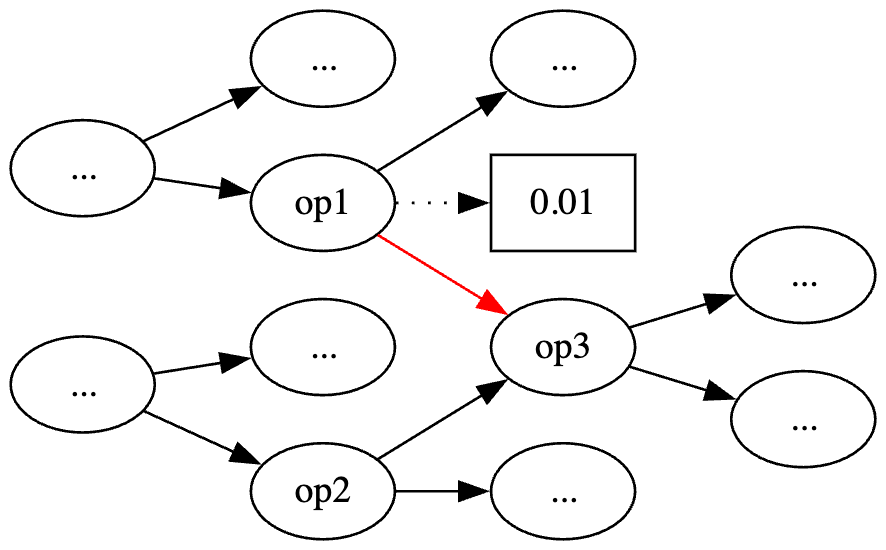
\includegraphics[width=6.5cm]{mgg_automl_zero_vag/mutations/const_to_connection.png}
  \caption{定数ノードを接続に置き換える突然変異の具体例. この例では, op1ノードと0.01が設定されている定数ノードの間のエッジを外して, op1をop3に接続する変化を示している.}
  \label{fig:mgg_automl_zero_vag:mutation:const_to_connection}
\end{figure}

\subsection{接続を定数ノードに置き換え}
接続を定数ノードに置き換える突然変異は, 複数の親ノードを持つノード$u \in U$とその親ノード$u_\mathrm{parent}$を一様ランダムに選択した上で, $u$と$u_\mathrm{parent}$の間のエッジを除去して, $u$の子ノードに定数ノードを割当てる操作である. ただし, 突然変異後にも妥当なアルゴリズムの条件を満たす$u$, $v$のみが選択対象であることに注意されたい. また, この突然変異操作は, 定数ノードを接続に置き換える操作の逆操作であると考えることができる. 接続を定数ノードに置き換える突然変異の具体例をFig.\ref{fig:mgg_automl_zero_vag:mutation:const_to_connection}に示す. この例では, op1ノードと親ノードを複数持つop3ノードの間のエッジを外して, op1の子ノードに0.01が設定されている定数ノードを割り当てている.

\begin{figure}
  \centering
  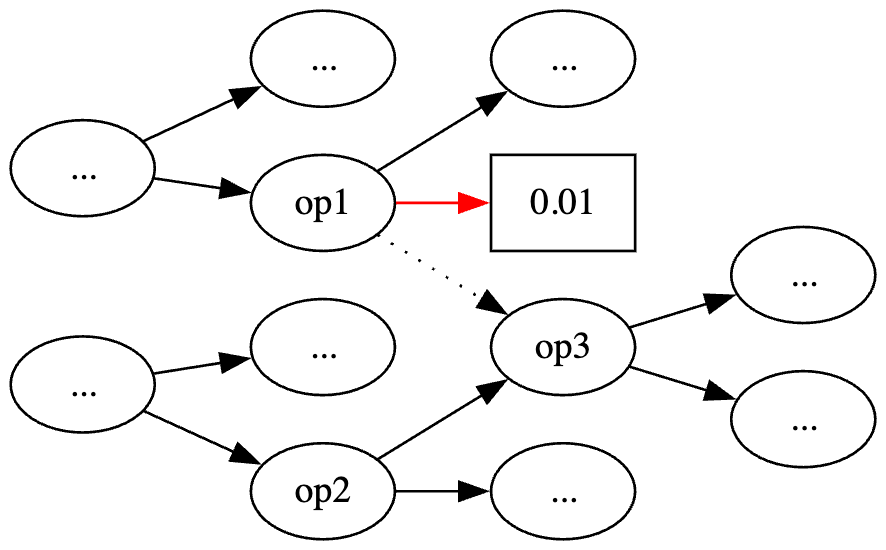
\includegraphics[width=6.5cm]{mgg_automl_zero_vag/mutations/connection_to_const.png}
  \caption{接続を定数ノードに置き換える突然変異の例. この例では, op1ノードと複数の親ノードを持つop3ノードの間のエッジを外して, op1の子ノードに0.01が設定されている定数ノードを割り当てている.}
  \label{fig:mgg_automl_zero_vag:mutation:connection_to_const}
\end{figure}

\subsection{接続関係の変更}
接続関係を変更する突然変異は, 複数の親ノードを持つノード$v$とその親ノード$u$を一様ランダムに選択した上で, $u$と$v$の間のエッジを除去して, $u$を別のノードと接続する操作である. ただし, 突然変異後にも妥当なアルゴリズムの条件を満たす$u$, $v$のみが選択対象であることに注意されたい. 接続関係を変更する突然変異の具体例を\ref{fig:mgg_automl_zero_vag:mutation:change_connection}に示す. この例では, op1ノードと親ノードを複数持つop4ノードの間のエッジを外して, op1ノードとop3ノードを接続している.

\begin{figure}
  \centering
  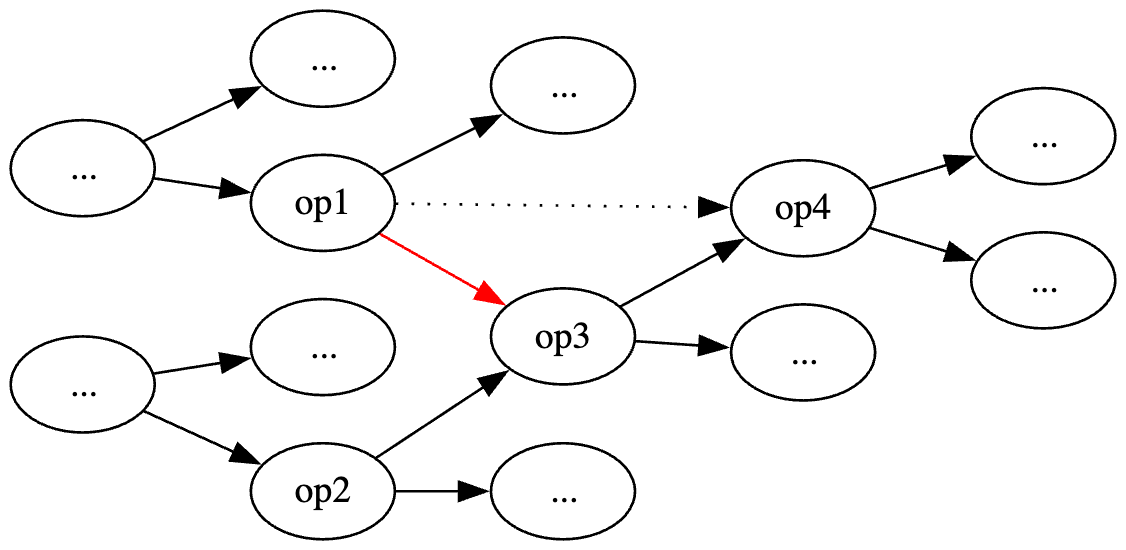
\includegraphics[width=8.2cm]{mgg_automl_zero_vag/mutations/change_connection.png}
  \caption{接続関係を変更する突然変異の具体例. この例では, op1ノードと親ノードを複数持つop4ノードの間のエッジを外して, op1ノードとop3ノードを接続している.}
  \label{fig:mgg_automl_zero_vag:mutation:change_connection}
\end{figure}

\subsection{部分グラフの再構築}

部分グラフの再構築は以下の手順で行われる.

\begin{enumerate}
  \item 選択する部分グラフの葉ノードを除くサイズ$s$を所与の確率分布$p_\mathrm{size}$に従って決定する.
  \item 部分グラフのルートノード$u_\mathrm{root}$を一様ランダムに決定する.
  \item 以下の条件を満たす$s-1$個の命令ノード$ u_\mathrm{op,1},u_\mathrm{op,2},u_{\mathrm{op},s-1} \in D_G(u_\mathrm{root})$を以下の条件を満たすように取得する.
  \begin{itemize}
    \item 任意の$ i $に対して, $u_\mathrm{op,i}$は命令ノードである.
    \item 任意の$ i $に対して, $u_\mathrm{op,i}$はNLPノードではない.
    \item 任意の$ i $に対して, $u_\mathrm{op,i}$は予測ノードではない.
    \item 任意の$ i $に対して, $u_\mathrm{root}$から$u_\mathrm{op,i}$への経路で, 経由点は$ u_\mathrm{op,1},u_\mathrm{op,2},u_{\mathrm{op},s-1}$のみであるものが存在する.
  \end{itemize}
  \item $u_\mathrm{root}$および$ u_\mathrm{op,1},u_\mathrm{op,2},u_{\mathrm{op},s-1}$とそれらの子ノードを含めた部分グラフを選択する.
  \item 選択された部分グラフをルートノードの型と終端ノードを保持した状態で以下の手順で再構築する.
  \begin{enumerate}
    \item ルートノードの命令を型を維持した状態で一様ランダムに変更する.
    \item 命令ノード拡張操作で1で決定したサイズになるまで命令ノードを追加する.
    \item 元の部分グラフの全ての終端ノードをノード指定接続操作で追加する.
  \end{enumerate}
\end{enumerate}

部分グラフの再構築を具体例を用いて説明する. サイズが2の部分グラフを, Fig.\ref{fig:mgg_automl_zero_vag:mutation:subgraph}の灰色の領域に示した. $s6$が部分グラフのルートノードであり, 他の部分グラフのノードは$s6$の子孫に含まれる. $s0$, $s1$, $s3$は, 部分グラフ内に子ノードを持たないので, 部分グラフの終端ノードである. また, $s4$はNLPノードでも, $s1$ノードでもなく, 親ノードは元のグラフを含めて1つである. そのため, Fig.\ref{fig:mgg_automl_zero_vag:mutation:subgraph}において灰色で示した部分グラフは, 再構成するための部分木の条件を満たしている. この部分グラフを突然変異させた結果をFig.\ref{fig:mgg_automl_zero_vag:mutation:mutated_subgraph}に示す. 突然変異の前と後で, 部分グラフのサイズ, ルートノードの型, 葉ノードに違いがないことに注意されたい.

\begin{figure}
  \centering
  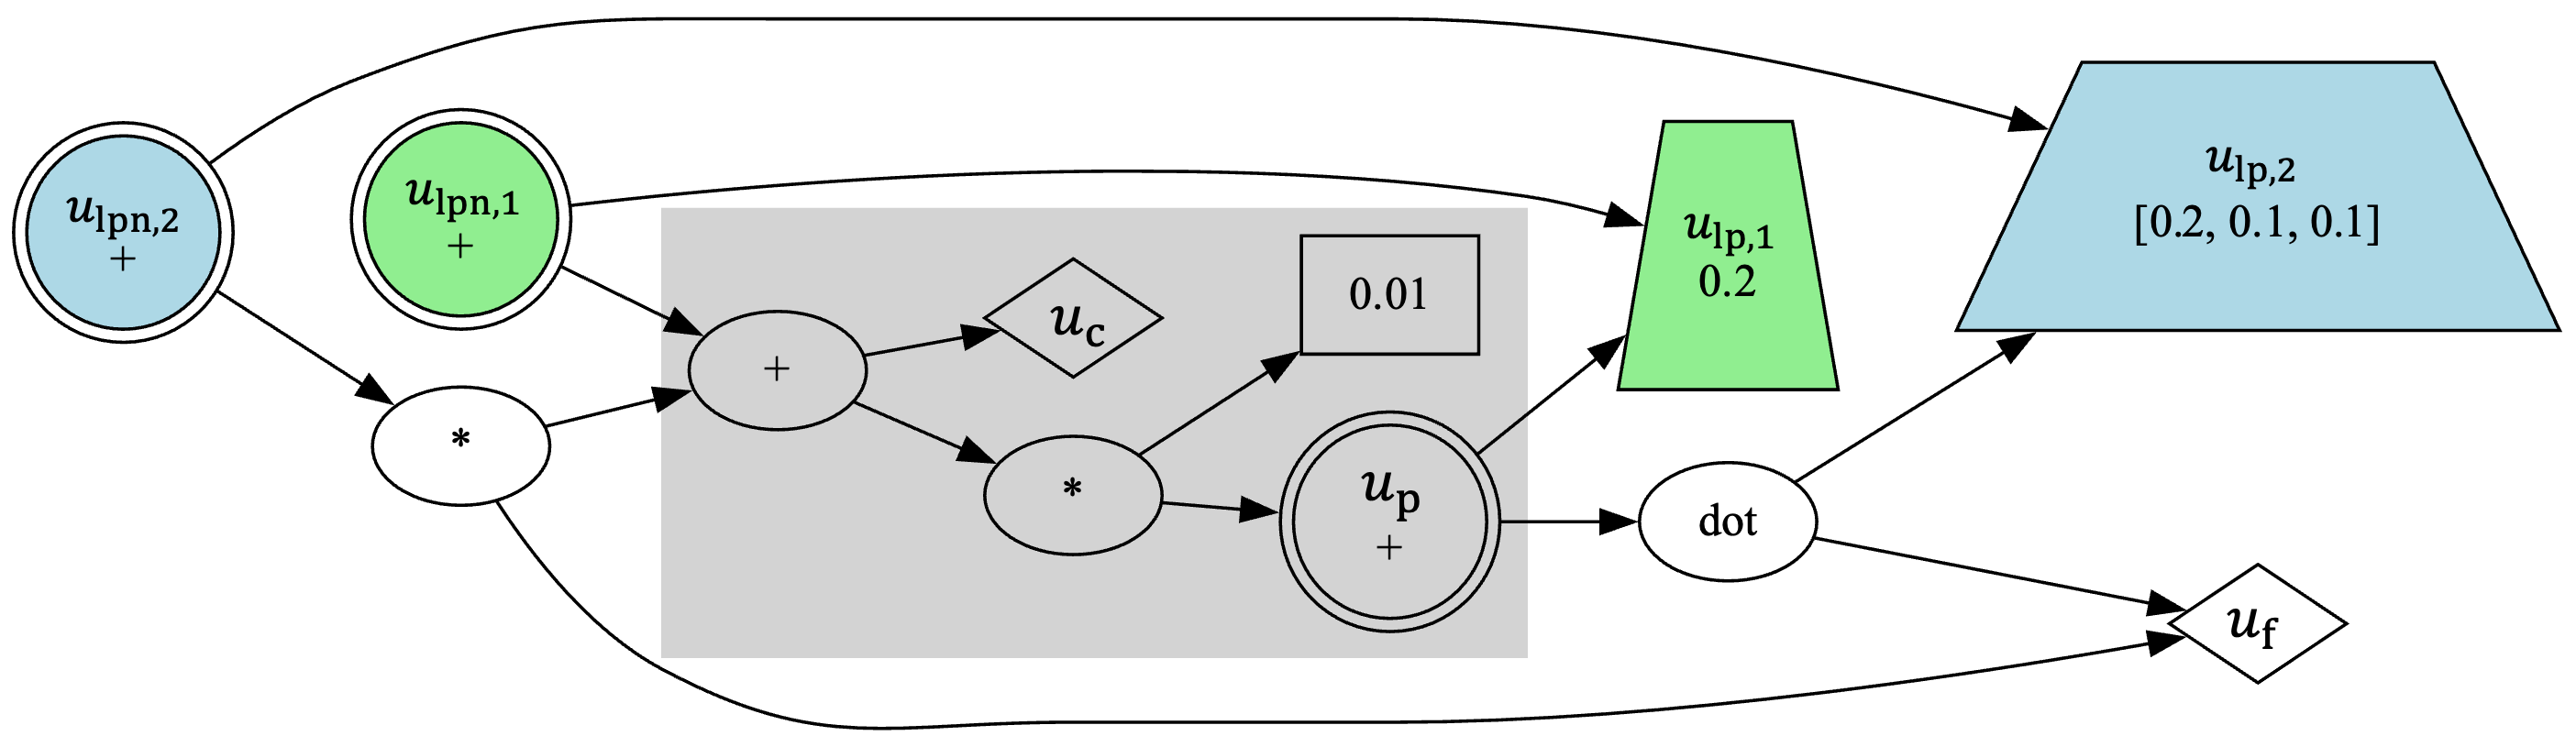
\includegraphics[width=14cm]{mgg_automl_zero_vag/mutations/subgraph.png}
  \caption{部分グラフの再構築の突然変異において選択される部分グラフの例. 灰色の範囲が部分グラフの全体を意味する. 本突然変異で選択する部分グラフでは, ルートノードと葉ノード以外のノードに, 親を複数持つノード, NLPノード, $s1$ノードを含めることはできない.}
  \label{fig:mgg_automl_zero_vag:mutation:subgraph}
\end{figure}

\begin{figure}
  \centering
  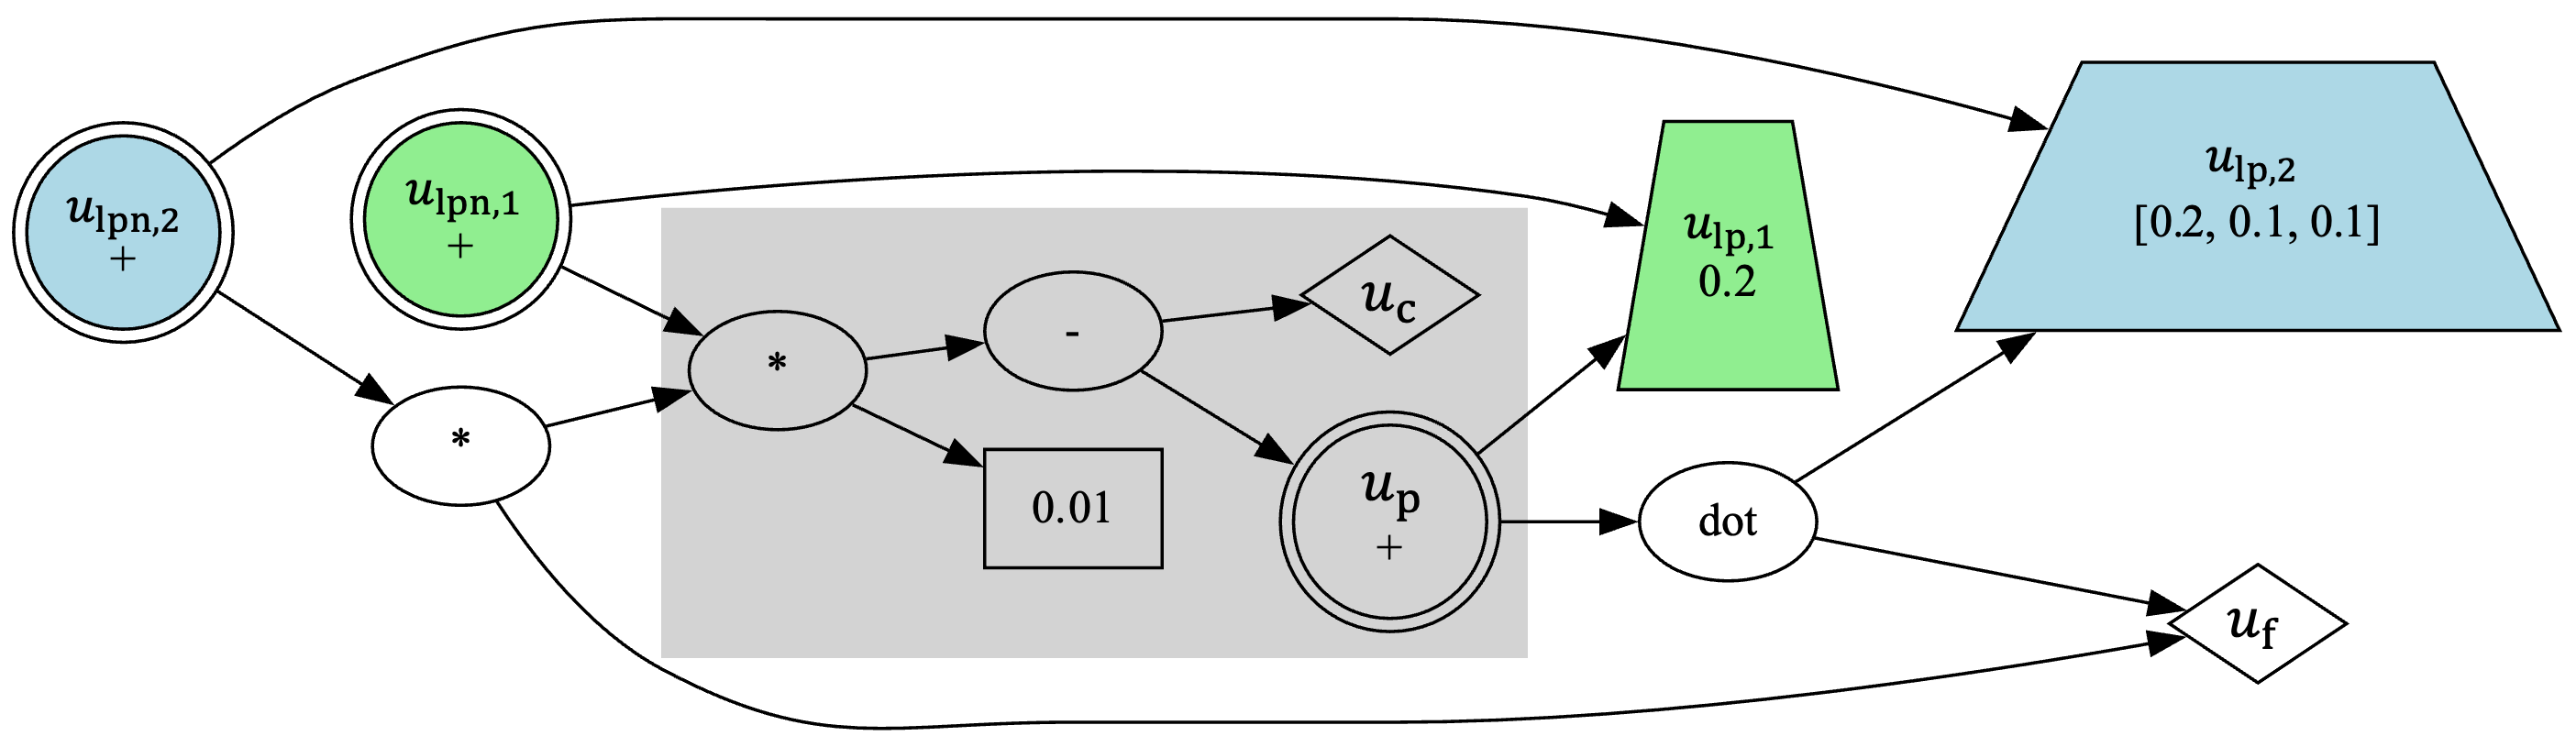
\includegraphics[width=14cm]{mgg_automl_zero_vag/mutations/mutated_subgraph.png}
  \caption{Fig.\ref{fig:mgg_automl_zero_vag:mutation:subgraph}に部分グラフの再構築の突然変異を適用した例. ルートノードの型と葉ノードは突然変異前と完全に同じであることに注意されたい.}
  \label{fig:mgg_automl_zero_vag:mutation:mutated_subgraph}
\end{figure}

部分グラフの再構築による突然変異は, 関数内の特定変数の計算に必要な部分命令列の変更に対応する. 既存手法では関数全体を書き換える突然変異が高頻度で発生し, 良質な部分命令列が破壊的に変更されていた. 一方, 提案手法における部分グラフの再構築は, 関数内の特定変数の計算に必要な部分のみを変更するため, 関数内の良質な部分命令列を維持した突然変異が可能となると考えられる.

\subsection{NLPノード$u_\mathrm{nlp}$と$D(u_\mathrm{nlp})$の再構築}

NLPノード$u_\mathrm{nlp}$と$D(u_\mathrm{nlp})$の再構築する突然変異では, NLPノード$u_\mathrm{nlp}$の計算にのみ利用されているノードと$C_\mathrm{nlp}(u_\mathrm{nlp}) < C_\mathrm{nlp}(u)$を満たすノード$u \in U$を削除した上で初期個体生成時と似た方法で再構築を行う. $u_\mathrm{nlp}$の計算にのみ利用されているノード除去は, 子ノードを再帰的に見ていき, 予測ノード$u_\mathrm{p}$, NLPノード, 親を複数持つノードが出現したら, それらのノードは除去せずに停止する. Fig.\ref{fig:mgg_automl_zero_vag:mutation:reconstruct_nlp}にNLPノード$v6$が選択された場合に, 除去されるノードおよびエッジを点線で示している. ノードを除去した後の再構築は, 第\ref{subsec:proposed:initialization:nlp}節で述べた構築方法を$k=C_\mathrm{nlp}(u_\mathrm{nlp})$から再度実行することで実現する. ただし, $k=C_\mathrm{nlp}(u_\mathrm{nlp}) + 1$以降は完全に同じだが, $k=C_\mathrm{nlp}(u_\mathrm{nlp})$では一部の処理が異なる. $k=C_\mathrm{nlp}(u_\mathrm{nlp})$においては, 除去されたNLPノードを初期化操作により再度初期化した上で, Algorithm \ref{algorithm:construct_nlp_node}の9行目から処理を開始する. ただし, $\mathrm{random}$関数では, 常に再構築の対象として$u_\mathrm{nlp}$が選択されるものとし, 9行目のfor文や25行目のfor文の最初の$i$の値は, 既に構築済みの他のノードに基づいて設定されるものとする.

\begin{figure}
  \centering
  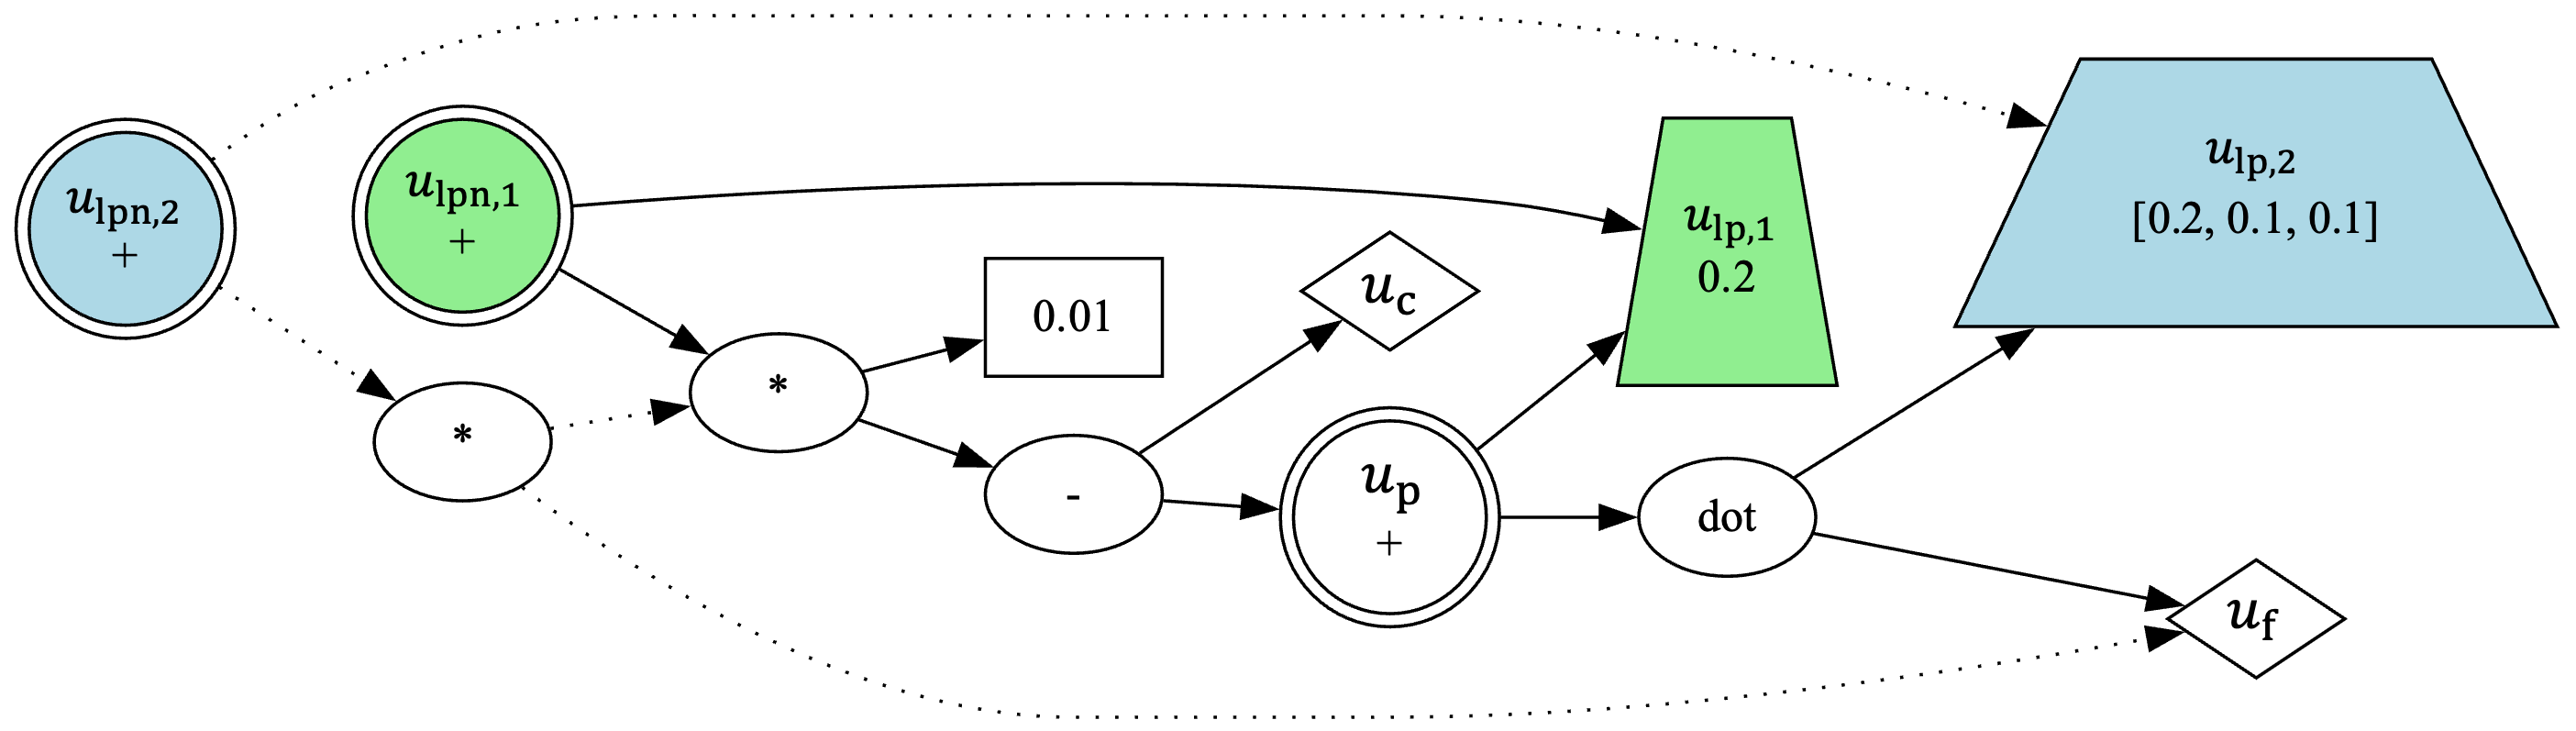
\includegraphics[width=14cm]{mgg_automl_zero_vag/mutations/reconstruct_nlp.png}
  \caption{NLPノード$v6$の再構築をする際に除去されるノード. 点線で囲まれたノードが除去されるノードであり, 点線で示されたエッジが除去されるエッジである. }
  \label{fig:mgg_automl_zero_vag:mutation:reconstruct_nlp}
\end{figure}

\subsection{予測ノード$u_\mathrm{p}$と$D(u_\mathrm{p})$の再構築}
予測ノード$u_\mathrm{p}$をルートとする部分グラフの再構築は, 初期個体生成と同等の操作である. 一般に, 機械学習アルゴリズムの予測式が変更される際には, 学習パラメータの構造が大きく変化するため, 既存のNLPノードを維持した突然変異は困難である. この再構築は破壊的な変異であるため, その選択確率を抑制し, 代わりに初期集団を大きくすることが望ましい. ただし, $s1$ノードの再構築による突然変異を完全に除外すると, NLP媒介数0の学習パラメータの構成変更が不可能となり, 探索空間が不当に制限される可能性がある点に注意されたい.

\section{多様性維持の工夫}\label{sec:proposed:diversity}

\subsection{世代交代モデルMGGの利用}

\begin{figure}[tbp]
  \centering
  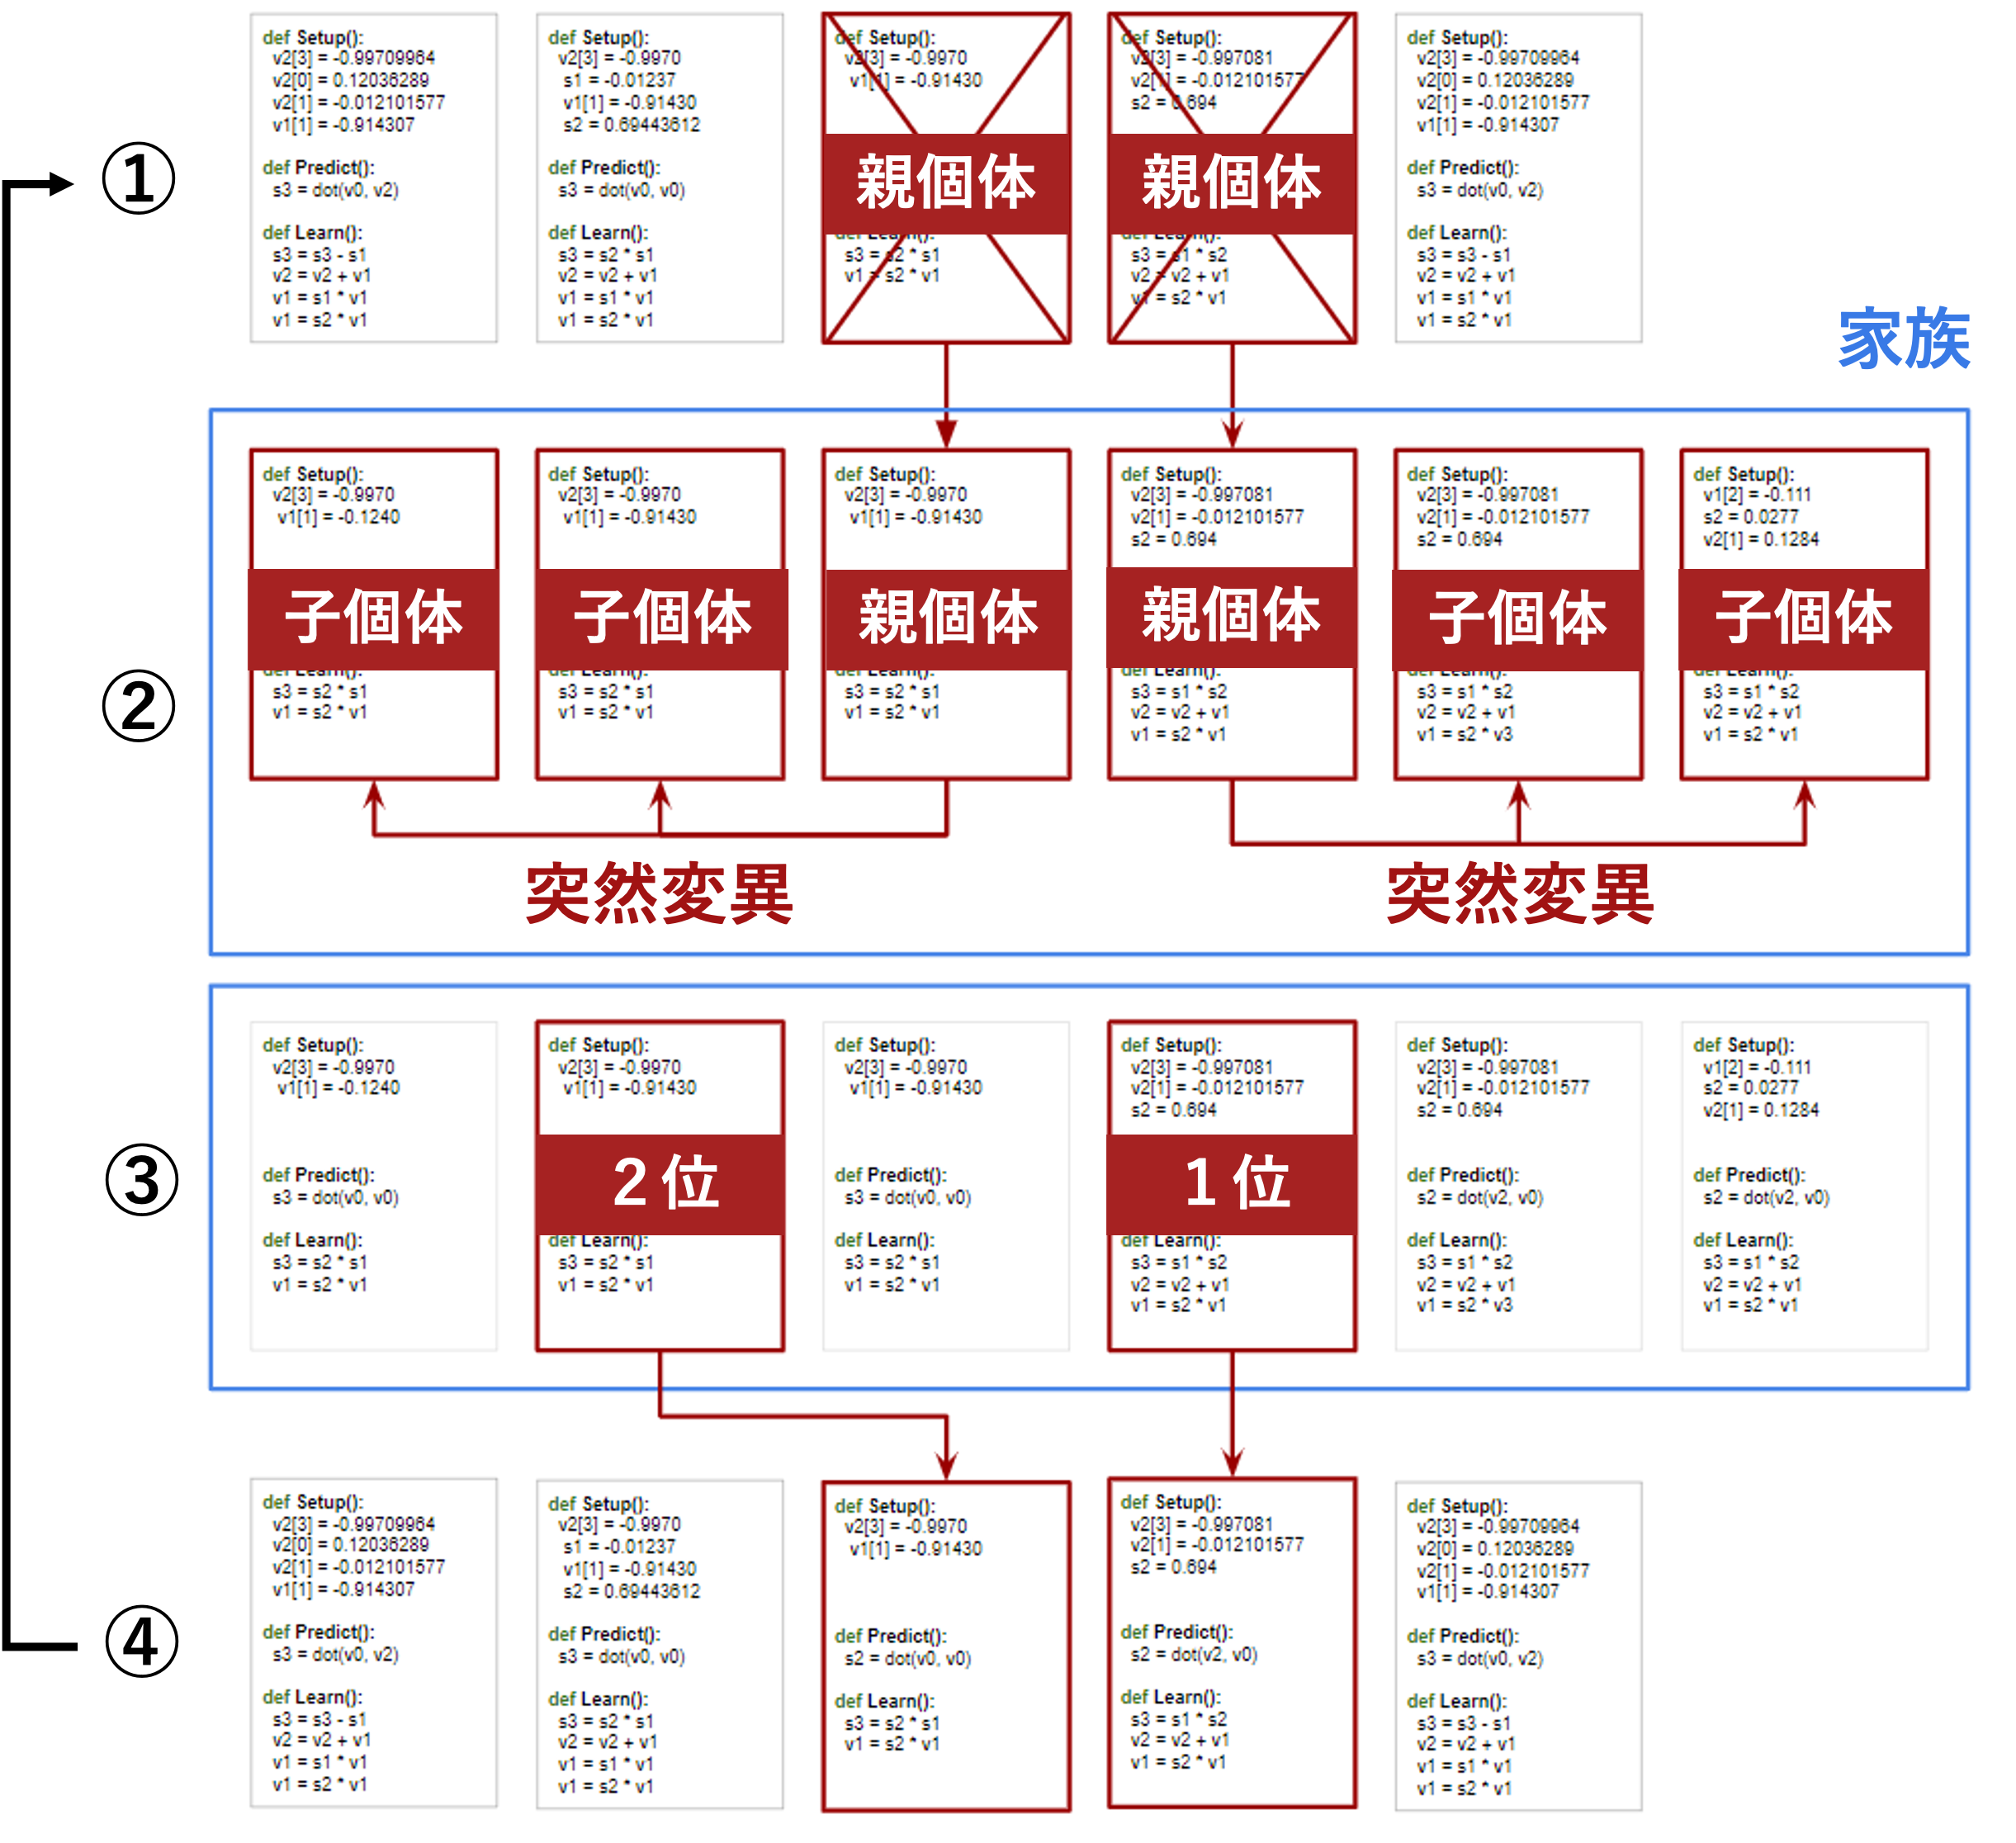
\includegraphics[width=14cm]{mgg_automl_zero_vag/ag/mgg.png}
  \caption{MGGによる世代交代の流れ}
  \label{fig:mgg}
\end{figure}

提案手法では, 集団の多様性を維持しやすくするため, RE-AutoML-Zeroと同様の方法で初期集団を生成した後に, Fig.\ref{fig:mgg}に示したMGGによる世代交代を繰り返し行う. 各世代交代では, STEP1で無作為に2つのアルゴリズム$p_a$, $p_b$を親個体として取り出し, STEP2で$p_a$を突然変異させた個体を$N_\mathrm{children} / 2$個, $p_b$を突然変異させた個体を$N_\mathrm{children} / 2$個つくり, 合計で$N_\mathrm{children}$個の子個体を生成する. その後のSTEP3,4では, 生成した$N_\mathrm{children}$個の子個体と親個体$p_a$, $p_b$を合わせた家族に対して生存選択で2つ個体を選択して集団に戻す. 生存選択の詳細については, 第\ref{subsec:prposed:diversity:survival_selection}節で説明する. 集団サイズ$N_\mathrm{pop}$, 子個体生成数$N_\mathrm{children}$はユーザパラメータである.

世代交代モデルをMGGに置き換えることで, 第\ref{subsec:problem:existing_problem:diversity}節で述べた3つの集団の多様性を低下させる要因に対処できると考えられる. MGGでは, Fig.\ref{fig:mgg}のSTEP1で淘汰される候補となった親個体も, Fig.\ref{fig:mgg}のSTEP3, 4の生存選択で集団に戻される可能性があるため, 集団内の個体が無条件で淘汰されることはない. また, Fig.\ref{fig:mgg}のSTEP1で無作為に複製選択するため, トーナメント選択のような強い選択圧がかかりにくいと考えられる. 加えて, STEP3, 4における生存選択で選ばれる個体が, 淘汰される候補である親個体の家族に限定されているため, 淘汰される個体と無関係な個体が次世代に引き継がれることが少ない.

\subsection{集団内の同一個体の排除}
本節では, 既存手法の同一のアルゴリズムが集団内に存在し, 集団の多様性が低下する問題への対処を説明する. 提案手法では, 同一なアルゴリズムを集団内から排除する工夫を導入する. 具体的には, 初期個体の生成時は初期集団内にグラフ構造が同一な個体が存在しないようにする. また, 子個体生成時には突然変異の特性によって, 排除するべきアルゴリズムが異なる. グラフ構造を変更する突然変異の場合は, 家族と集団に同一のグラフ構造を持つ個体が存在しないようにする. 定数ノードやLPノードに割り当てられているパラメータを変更する突然変異の場合は, 家族と集団にグラフ構造とパラメータがどちらも同一となる個体が存在しないようにする.

提案手法で導入する同一個体の排除は, アルゴリズムの探索の特徴を踏まえると妥当であると考えられる. 一般に, グラフ構造に変化すると, 変化前のグラフ構造で最適化された定数や学習パラメータの初期値は, 無意味になることが多い. そのため, 集団ではグラフ構造を幅広く探索していきつつ, 有望なアルゴリズムの定数値や学習パラメータの初期値を最適化していくことが重要であると考えられる. 故に, 初期集団において定数値や学習パラメータの初期値のみが異なり, グラフ構造が同一の個体が存在する意義は少ないと考えられる. また, 突然変異によって, グラフ構造が変わった結果, 集団内にグラフ構造が同一な個体が存在する場合は, 既に集団内に存在する個体の方が定数値や学習パラメータの初期値が最適化されていると考えられる. そのため, 集団内に存在する個体のみを残しておけば良いと考えられる. 一方で, 定数値や学習パラメータの初期値が突然変異によって変わった場合は, グラフ構造, 定数値, 学習パラメータの初期値が完全に同一な個体が存在する場合以外は, 新たな有望な個体である可能性があるため, 排除することは避けるべきである.

\subsection{希少度に基づく生存選択} \label{subsec:prposed:diversity:survival_selection}
探索序盤における類似個体や同一個体の急激な増加は, 改善の見込みがある有望な個体の淘汰につながるため, MGGで利用する生存選択は慎重に決定する必要がある. 佐藤らのMGGの生存選択では, 家族の中で最良適合度を持つ個体とルート選択で選ばれた個体を集団に戻す方法が採用されている\cite{mgg}. しかし, この生存戦略は子個体が改善する見込みが高い連続値の最適化において有力な手法であり, 子個体が改悪している可能性が高い離散最適化においては適切ではない可能性が高い. 離散最適化におけるMGGの生存選択では, 家族の適合度の上位2つの個体を集団に戻す手法も一般的である. 一方, この手法では初期段階で適合度の良い局所解に収束する可能性を高めてしまうという課題がある.

提案手法では, 多様性維持と探索効率のバランスを取るための生存選択手法として, 集団内の希少度を利用する方法を提案する. 具体的には, 家族において最も適合度が高い個体と以下のスコア$S(a)$が最大となる個体$\arg \min_a S(a, \mathcal{T}_\mathrm{search}, P)$を集団に戻す.

$$
 S(a, \mathcal{T}_\mathrm{search}, P) = (1-w_\mathrm{r}) F(a, \mathcal{T}_\mathrm{search}) + w_\mathrm{r} R(a, P), \quad
 R(a, P) = \frac{1}{N_{\mathrm{discrete}}(P, a) + 1}
$$

\noindent
ここで, $a$は個体, $F(a, \mathcal{T}_\mathrm{search})$は$\mathcal{T}_\mathrm{search}$に対するアルゴリズムの適合度, $w_\mathrm{r}$はアルゴリズムの希少度をどの程度重要視するかの重み, $N_\mathrm{discrete}(P, a)$は集団$P$において$a$とグラフ構造が同一の個体の数を表す. $R(a, P)$は集団$P$における個体$a$の希少度を意味しており, 集団内の個体が少ないほど大きい値となる. スコア$S(a, \mathcal{T}_\mathrm{search}, P)$に基づいて, 生存選択を行うことで, 探索序盤で同一個体や類似個体が急速に増える問題に対処できると考えられる.

\subsection{詳細なアルゴリズム}
Algorithm \ref{algorithm:mgg_automl_zero}に提案手法の世代交代アルゴリズムを示す. このアルゴリズムは, タスク集合$\mathcal{T}_\mathrm{search}$, 集団サイズ$N_\mathrm{pop}$, 子個体生成数$N_\mathrm{children}$, 最大評価回数$ N_\mathrm{eval}$を入力として受け取り, 探索の結果発見されたアルゴリズムを出力する.

\begin{breakablealgorithm}
  \caption{提案手法の世代交代アルゴリズム}
  \label{algorithm:mgg_automl_zero}
  \begin{algorithmic}[1]
    \REQUIRE タスク集合$\mathcal{T}_\mathrm{search}$, 集団サイズ$N_\mathrm{pop}$, 子個体生成数$N_\mathrm{children}$, 最大評価回数$ N_\mathrm{eval}$
    \ENSURE 発見されたアルゴリズム
    \STATE $\mathrm{eval\_num} \leftarrow 0 $
    \STATE $P \leftarrow \emptyset $
    \FOR{$ i = 1 $ to $ N_\mathrm{pop}$}
    \WHILE{true}
    \STATE $\mathrm{algorithm} \leftarrow  \mathrm{generate\_algorithm\_graph}()$
    \IF{$\mathrm{is\_unique\_structure}(P, \mathrm{algorithm})$}
    \STATE break
    \ENDIF
    \ENDWHILE
    \STATE $\mathrm{fitness} \leftarrow  F(a, \mathcal{T_\mathrm{search}})$
    \STATE $\mathrm{eval\_num} \leftarrow \mathrm{eval\_num} + 1 $
    \STATE $\mathrm{individual} \leftarrow  (\mathrm{algorithm}, \mathrm{fitness}) $
    \STATE $P \leftarrow P \cup \{ \mathrm{individual} \} $
    \ENDFOR
    \WHILE{$\mathrm{eval\_num} < N_\mathrm{eval}$}
    \STATE $\mathrm{parent1} \leftarrow \mathrm{random}(P)$
    \STATE $ \mathrm{parent2} \leftarrow \mathrm{random}(P)$
    \STATE $ F = \{ \mathrm{parent1}, \mathrm{parent2} \} $
    \STATE $ P \leftarrow P \setminus F $
    \FOR{$i = 1$ to $N_\mathrm{children}$}
    \IF{$i \equiv 0 \pmod{2}$}
    \STATE $\mathrm{parent} \leftarrow \mathrm{parent1}$
    \ELSE
    \STATE $\mathrm{parent} \leftarrow \mathrm{parent2}$
    \ENDIF
    \WHILE{true}
    \STATE $\mathrm{algorithm} \leftarrow \mathrm{copy}(\mathrm{parent})$
    \STATE $(\mathrm{algorithm}, \mathrm{mutation\_type}) \leftarrow \mathrm{mutate}(\mathrm{algorithm})$
    \IF{$\mathrm{mutation\_type} = \mathrm{STRUCTURE}$ \\ \qquad and $\mathrm{is\_unique\_structure}(P \cup F, \mathrm{algorithm})$}
    \STATE break
    \ELSIF{$\mathrm{mutation\_type} = \mathrm{PARAMETER}$ \\ \qquad and $\mathrm{is\_unique}(P \cup F, \mathrm{algorithm})$}
    \STATE break
    \ENDIF
    \ENDWHILE
    \STATE $\mathrm{fitness} \leftarrow  F(\mathrm{algorithm}, \mathcal{T_\mathrm{search}})$
    \STATE $\mathrm{eval\_num} \leftarrow \mathrm{eval\_num} + 1 $
    \STATE $\mathrm{individual} \leftarrow  (\mathrm{algorithm}, \mathrm{fitness}) $
    \STATE $F \leftarrow F \cup \{ \mathrm{individual} \} $
    \ENDFOR
    \STATE $\mathrm{individual1} \leftarrow  \mathrm{get\_best\_fitness(F)}$
    \STATE $F \leftarrow F \setminus \{\mathrm{individual1} \}$
    \STATE $\mathrm{individual2} \leftarrow  \mathrm{get\_best\_score(F)}$
    \STATE $P \leftarrow P \cup \{\mathrm{individual1}, \mathrm{individual2}\}$
    \ENDWHILE
    \STATE $\mathrm{best\_algorithm} \leftarrow  \mathrm{get\_best\_fitness}(P)$
    \RETURN $\mathrm{best\_algorithm}$
  \end{algorithmic}
\end{breakablealgorithm}

Algorithm \ref{algorithm:mgg_automl_zero}の詳細な説明を以下に示す.

\begin{description}
  \item[1行目] 評価回数のカウンターを0で初期化する.
  \item[2行目] 集団$P$を初期化する.
  \item[3-14行目] グラフ構造が同一の個体が集団内に含まれないように, 初期集団個体を生成して, 適合度を計算する.
  \begin{description}
    \item[4-9行目] 集団$P$に存在しないグラフ構造が得られるまで, 初期個体を生成し続ける.
    \begin{description}
      \item[5行目] 第\ref{sec:proposed:initialization}説で述べた初期個体生成方法で個体を生成する関数$\mathrm{generate\_algorithm\_graph}$を用いてアルゴリズムグラフを生成する.
      \item[6-8行目] 集団$P$に同一のグラフ構造をもつアルゴリズムグラフが存在する場合は個体の生成を行う. 同一のグラフ構造をもつアルゴリズムグラフの存在性は, $\mathrm{is\_unique\_structure}$関数によって判定される.
    \end{description}
    \item[10行目] アルゴリズムグラフを評価して適合度を計算する.
    \item[11行目] 評価回数のカウンターをインクリメントする.
    \item[12行目] アルゴリズムグラフと適合度のペアを個体として代入する.
    \item[13行目] 集団に個体を追加する.
  \end{description}
  \item[15行目] 評価回数の上限に到達するまで世代交代を繰り返す.
  \begin{description}
    \item[16行目] 1つ目の親個体を一様ランダムに取得する.
    \item[17行目] 2つ目の親個体を一様ランダムに取得する.
    \item[18行目] 家族の集合を2つの親個体で初期化する.
    \item[19行目] 選択された2つの親個体を集団から削除する.
    \item[20-39行目] 所与の個数に到達するまで子個体を生成する.
    \begin{description}
      \item[21-25行目] 各親個体から生成する子個体数を揃えられるように親個体を選択する.
      \item[26-34行目] 重複排除の条件が満たされるまで子個体生成を繰り返す.
      \begin{description}
        \item[27行目] 親個体をコピーする.
        \item[28行目] 第\ref{sec:proposed:mutation}節の突然変異による子個体生成を行う$\mathrm{mutate}$関数を実行する. $\mathrm{mutate}$の返り値は, 突然変異後のアルゴリズムグラフと突然変異の種類である. 突然変異の種類は, 定数ノードの定数値の変更とLPノードの学習パラメータの初期値の変更の場合は$\mathrm{PARAMETER}$となり, それ以外の場合は$\mathrm{STRUCTURE}$となる.
        \item[29-31行目] グラフ構造の変更を伴う突然変異の場合は, 家族と集団に同一のグラフ構造を持つ個体が存在した場合は子個体の生成をやり直す. 同一のグラフ構造をもつアルゴリズムグラフの存在性は, $\mathrm{is\_unique\_structure}$関数によって判定される.
        \item[31-33行目] パラメータの変更のみの突然変異の場合は, 家族と集団に完全に同一の個体が存在した場合は子個体の生成をやり直す. 完全同一のアルゴリズムグラフの存在性は, $\mathrm{is\_unique}$関数によって判定される.
      \end{description}
      \item[35行目] アルゴリズムグラフを評価して適合度を計算する.
      \item[36行目] 評価回数のカウンターをインクリメントする.
      \item[37行目] アルゴリズムグラフと適合度のペアで子個体として代入する.
      \item[38行目] 家族$F$に作成した子個体を追加する.
    \end{description}
    \item[40行目] 家族$F$の中で最も適合度が高い個体を取得する.
    \item[41行目] 家族$F$から最も適合度が高い個体を除去する.
    \item[42行目] 家族$F$の中で最もスコア$S(a,\mathcal{T}_\mathrm{search}, P)$が高い個体を取得する関数$\mathrm{get\_best\_score}$を実行して, 希少度と適合度を考慮したスコアが最も高い個体を取得する.
    \item[43行目] 集団に最も適合度が高い個体と希少度と適合度を考慮したスコア$S(a,\mathcal{T}_\mathrm{search}, P)$が最も高い個体を戻す.
  \end{description}
  \item[45行目] 集団の中で最も適合度の高い個体を取得する.
  \item[46行目] 集団の中で最も適合度の高い個体を返却する.
\end{description}

\chapter{実験} \label{chap:exp}

\section{目的}\label{sec:exp:purpose}

本実験の目的は, 回帰アルゴリズムや分類アルゴリズムの探索問題をローカルPCの少ない計算リソース上で実行し, 提案手法と既存手法の探索性能を比較をすることである. 既存手法であるEstebanらの手法RE-AutoML-Zero\cite{automl_zero}に比べて, 提案手法のMGG-AutoML-Zero+VAGの方が, 所与の評価回数で高い適合度のアルゴリズムが得られることを確認する.

\section{比較手法}\label{sec:exp:compair_method}
既存手法であるEstebanらの手法RE-AutoML-Zeroと提案手法のMGG-AutoML-Zero+VAGを比較する.

\section{ベンチマーク問題}\label{sec:exp:benchmark}

\subsection{問題設定の概要}

本実験では, Table.\ref{table:exp_benchmarks}に示した合計24種類のベンチマーク問題を利用して実験を行う. 回帰問題と分類問題それぞれで, 線形, アフィン, 非線形の特性を持つ問題を用いる. また, それぞれの問題に対して, ノイズがない場合とノイズが正規分布$N(0,0.1)$に従う場合の計2種類の問題を用意する.

\begin{table*}[tbp]
  \caption{実験で利用する合計24種類のベンチマーク問題. 回帰問題と分類問題それぞれで, 線形, アフィン, 非線形の特性を持つ問題を利用. また, それぞれの問題に対して, ノイズがない場合とノイズが正規分布$N(0,0.1)$に従う場合の計2種類の問題を用意.}
  \label{table:exp_benchmarks}
  \centering
  \begin{tabular}{|l|l||cc|}
    \hline
    \multicolumn{2}{|c||}{問題設定} & \multicolumn{2}{|c|}{ノイズ} \\
    \hline
    \hline
    \multirow{3}{*}{回帰問題}
    & 線形 &  なし & $N(0,0.1)$ \\
    & アフィン& なし & $N(0,0.1)$ \\
    & 非線形 &  なし & $N(0,0.1)$ \\
    \hline
    \multirow{3}{*}{分類問題}
    & 線形 &  なし & $N(0,0.1)$ \\
    & アフィン& なし & $N(0,0.1)$ \\
    & 非線形&  なし & $N(0,0.1)$ \\
    \hline
  \end{tabular}
\end{table*}

\begin{table*}[tbp]
  \caption{回帰問題のベンチマーク問題. 問題設定における探索に利用するタスクの数$\left|\mathcal{T}_\mathrm{search} \right|$, 最終評価に利用するタスクの数$\left|\mathcal{T}_\mathrm{eval} \right|$, 各タスクの学習用データの数$\left|D_\mathrm{train}\right|$, 各タスクの検証データの数$\left|D_\mathrm{valid}\right|$}
  \label{table:regression_exp_benchmark}
  \centering
  \begin{tabular}{|c|c|c|c|}
    \hline
    & 線形回帰問題 & アフィン回帰問題 & 非線形回帰問題 \\
    \hline
    \hline
    $\left|\mathcal{T}_\mathrm{search} \right|$ & 10 & 10 & 100 \\
    $\left|\mathcal{T}_\mathrm{eval} \right|$ & 10 & 10 & 100 \\
    $\left|D_\mathrm{train}\right|$ & 1000 & 1000 & 1000 \\
    $\left|D_\mathrm{valid}\right|$ & 100 & 100 & 100 \\
    \hline
  \end{tabular}
\end{table*}

\subsection{タスク集合の構成}
本節では, 各問題設定のタスク集合の構成方法について説明する. 全ての問題設定で共通して, 探索用のタスク集合$\mathcal{T}_\mathrm{search}$および最終評価用のタスク集合$\mathcal{T}_\mathrm{eval}$に含まれるタスクは10個とした. また, タスク$T \in \mathcal{T}$の学習データと検証用データの個数は, それぞれ1000個と100個として, エポック数は1, 問題の次元は4に設定した. それぞれのタスクの入力ベクトル$\bm{x}_j$と正解ラベル$y_j$の構成方法を問題設定ごとに以下に示す. 以下の説明において, $\bm{v} \sim \bm{N}(N,0)$はベクトル$\bm{v}$が各要素が平均$N$, 分散$0$の正規分布に従うことを意味し, $U(x)$は$x \leq 0$の時に$0$, $x > 0$の時に$1$となるステップ関数, $n_j$はTable.\ref{table:exp_benchmarks}に示したノイズの確率分布に従う変数である.

\subsubsection{線型回帰問題}
$$
  \bm{x}_j \sim \bm{N}(0, 1), \quad y_j = \bm{w} \cdot \bm{x}_j + n_j \quad
  \bm{w} \sim \bm{N}(0, 1)
$$

\subsubsection{アフィン回帰問題}
$$
  \bm{x}_j \sim \bm{N}(0, 1), \quad y_j = \bm{w}, \cdot \bm{x}_j + u + n_j,\quad \bm{w} \sim \bm{N}(0, 1), \quad u \sim N(0, 1)
$$

\subsubsection{非線形回帰問題}
非線形回帰タスクは, 中間層が1層4ノードのランダムな重みのニューラルネットワークで, 中間層の出力を$\bm{v}_{j}=\left(v_{j, 1}, v_{j, 2}, v_{j, 3}, v_{j, 4}\right)^{\mathrm{T}}$とすると, 入力ベクトル$\bm{x}_j$と正解ラベル$y_j$は以下のように構成される.

\begin{gather*}
  \bm{x}_j \sim \bm{N}(0, 1), \quad v_{j, k} = \mathrm{ReLU}\left(\bm{x}_{j} \cdot \bm{w}_{k}\right), \quad y_j = \bm{v}_{j} \cdot \bm{w}_{\mathrm{out}} + n_j \\
\bm{w}_{k} \sim \bm{N}(0, 1), \quad \bm{w}_{\mathrm{out}} \sim \bm{N}(0, 1)
\end{gather*}

\subsubsection{線型分類問題}
$$
  \bm{x}_j \sim \bm{N}(0, 1), \quad y_j = U(\bm{w} \cdot \bm{x}_j + n_j) \quad
  \bm{w} \sim \bm{N}(0, 1)
$$

\subsubsection{アフィン分類問題}
$$
  \bm{x}_j \sim \bm{N}(0, 1), \quad y_j = U(\bm{w} \cdot \bm{x}_j + u + n_j),\quad \bm{w} \sim \bm{N}(0, 1), \quad u \sim N(0, 1)
$$

\subsubsection{非線形分類問題}
非線形回帰タスクは, 中間層が1層4ノードのランダムな重みのニューラルネットワークで, 中間層の出力を$\bm{v}_{j}=\left(v_{j, 1}, v_{j, 2}, v_{j, 3}, v_{j, 4}\right)^{\mathrm{T}}$とすると, 入力ベクトル$\bm{x}_j$と正解ラベル$y_j$は以下のように構成される.
\begin{gather*}
  \bm{x}_j \sim \bm{N}(0, 1), \quad v_{j, k} = \mathrm{ReLU}\left(\bm{x}_{j} \cdot \bm{w}_{k}\right), \quad y_j = U(\bm{v}_{j} \cdot \bm{w}_{\mathrm{out}} + n_j) \\
\bm{w}_{k} \sim \bm{N}(0, 1), \quad \bm{w}_{\mathrm{out}} \sim \bm{N}(0, 1)
\end{gather*}

\subsection{Normalize / Loss / Rescale 関数の設定} \label{sec:exp:functions}

本節では, アルゴリズムを評価する際に利用するNormalize関数, Loss関数, Rescale関数の設定について説明する. 各関数の詳細は, 第\ref{subsec:problem:existing_method:algorithm_eval}節を参照されたい.

回帰問題の Normalize関数, Loss関数, Rescale関数の設定を以下に示す.
\begin{eqnarray*}
\mathrm{Normalize}(s1) &=& s1 \\
\mathrm{Loss}(y, s1) &=& \left|y - s1\right| \\
\mathrm{Rescale}(l) &=& 1 - \frac{2}{\pi} \arctan\left(\sqrt{l}\right)
\end{eqnarray*}
\noindent
回帰問題においては, 予測ラベルをそのまま利用し, 二乗誤差を計算するように設定している. 適合度が高いほど良いアルゴリズムであるため, Rescale関数では, 損失関数の平均値を$[0,1]$に変換した上で, 1が高い適合度となるように逆転している.

分類問題のNormalize関数, Loss関数, Rescale関数の設定を以下に示す.
\begin{eqnarray*}
\mathrm{Normalize}(s1) &=& \mathrm{sigmoid}(s1) \\
\mathrm{Loss}(y, s1) &=&
\begin{cases}
  1 & |y-s1| \geq 0.5 \\
  0 & |y-s1| < 0.5
\end{cases} \\
\mathrm{Rescale}(l) &=& 1 - l
\end{eqnarray*}
\noindent
分類問題においては, 予測ラベルを分類確率に変換するために, Normalize関数にsigmoid関数を適用している. また, Loss関数は分類確率に基づいて分類した結果, 正しい分類であれば0, 誤った分類であれば1を返すように設定している. 適合度が高いほど良いアルゴリズムであるため, Rescale関数では1から誤分類率を引いた分類成功率を返すように設定している.

\section{評価基準}\label{sec:proposed:exp:eval}

本実験では, それぞれの問題設定で乱数を変えて10試行の実験を行い, 所与の評価回数までに発見されたアルゴリズムの適合度の平均値を評価基準とする. 第\ref{sec:exp:functions}説の定義より, 適合度は回帰問題の場合であれば全てのタスクの検証データに対して完全に誤差なしで回帰できた場合に1, 分類問題であれば全てのタスクの検証データを正しく分類できた場合に1となる. しかし, 一般には学習データと検証データは独立であるため, 完全な適合度1を達成することは難しい. また, 各実験における打ち切り適合度は0.999, 打ち切り評価回数は線形回帰/分類の問題では20,000回, アフィン回帰/分類の問題では2,000,000回, 非線形回帰/分類の問題では20,000,000回とした.

\section{実験設定}\label{sec:proposed:exp:setting}

本節では, 既存手法と提案手法のユーザパラメータの設定について説明する. 本実験は, 既存手法と提案手法の探索性能を比較することが目的なので, EstebanらのSection 4.1の実験と同様, それぞれの問題設定に対して良質なアルゴリズムを再現する上で必要な命令に限定した\cite{automl_zero}. 具体的には, 各問題に対する命令セットについては, Table.\ref{table:exp
:setting:ops}に示した通りに限定する. 各命令の詳細は, 付録\ref{chap:ops}を参照されたい. 命令セット以外の既存手法と提案手法のユーザパラメータは, それぞれTable.\ref{table:exp:setting:conventional}とTable.\ref{table:exp:setting:proposed}に示した値を用いた. 既存手法における設定値は, EstebanらのSection 4.1の実験と同じ値に設定した\cite{automl_zero}. 本実験では, 命令数が固定されているため, 命令を増減する突然変異に関しては, 既存手法および提案手法のいずれでも利用しないものとする.

\begin{table*}[tbp]
  \caption{実験で利用する命令セット. これらの命令セットはEstebanらのSection 4.1の実験と同様に設定している\cite{automl_zero}. 各命令の詳細は, 付録\ref{chap:ops}を参照されたい.}
  \label{table:exp
  :setting:ops}
  \centering
  \begin{tabular}{|l|l|l|}
    \hline
    問題設定 & 関数 & 命令セット \\
    \hline
    \hline
    \multirow{3}{*}{線形}
    & Setup &  OP56, OP57 \\
    & Predict, $\mathrm{OP}^{(0)}$ & OP27  \\
    & Learn, $\mathrm{OP}^{(1)}$ &  OP2, OP3, OP18, OP23 \\
    \hline
    \multirow{3}{*}{アフィン}
    & Setup &  OP56, OP57 \\
    & Predict, $\mathrm{OP}^{(0)}$ & OP1, OP27  \\
    & Learn, $\mathrm{OP}^{(1)}$&  OP1, OP2, OP3, OP18,
    OP23 \\
    \hline
    \multirow{3}{*}{非線形}
    & Setup & OP56, OP63, OP64 \\
    & Predict, $\mathrm{OP}^{(0)}$ & OP27, OP31, OP48 \\
    & Learn, $\mathrm{OP}^{(1)}$& OP2, OP3, OP16, OP18, OP23, OP25, OP28, OP40  \\
    \hline
  \end{tabular}
\end{table*}

\begin{table*}[tbp]
  \caption{既存手法の回帰問題におけるハイパーパラメータの設定値. これらの設定値はEstebanらのSection 4.1の実験と同じ値に設定している\cite{automl_zero}.}
  \label{table:exp:setting:conventional}
  \centering
  \begin{tabular}{|c|c|c|c|c|c|c|c|}
    \hline
    \multicolumn{3}{|c|}{パラメータ} & \multicolumn{3}{c|}{設定値} \\
    \hline
    \multicolumn{2}{|c|}{名前} & 数式表記 & 線形 & アフィン & 非線形 \\
    \hline
    \hline
    \multicolumn{2}{|c|}{集団サイズ} & $N_\mathrm{pop}$ & 1000 & 1000 & 1000 \\
    \hline
    \multicolumn{2}{|c|}{トーナメントサイズ} & $K$ & 10 & 10 & 10 \\
    \hline
    \multicolumn{2}{|c|}{突然変異確率} & $p_\mathrm{mutate}$ & 0.9 & 0.9 & 0.9 \\
    \hline
    \multirow{3}{*}{アドレス数}
    & スカラー & - & 4 & 5 & 4 \\
    & ベクトル & - & 3 & 3 & 8 \\
    & 行列 & - & 1 & 1 & 2 \\
    \hline
    \multirow{3}{*}{命令数}
    & Setup      & - & 5 & 6 & 21 \\
    & Predict    & - & 1 & 2 & 3 \\
    & Learn      & - & 4 & 6 & 9 \\
    \hline
  \end{tabular}
\end{table*}

\begin{table*}[tbp]
  \caption{提案手法におけるハイパーパラメータの設定値.}
  \label{table:exp:setting:proposed}
  \centering
  \begin{tabular}{|l|c|c|c|c|c|c|}
    \hline
    \multicolumn{2}{|c|}{パラメータ} & \multicolumn{3}{c|}{設定値} \\
    \hline
    名前 & 数式表記 & 線形 & アフィン & 非線形 \\
    \hline
    \hline
    集団サイズ    & $N_\mathrm{pop}$ & 1000 & 1000 & 10000 \\
    \hline
    子個体生成数  & $K$ & 100 & 100 & 1000 \\
    \hline
    \multirow{2}{*}{命令数}
    & $N_\mathrm{OP}^{(0)}$ & 1 & 2 & 3 \\
    & $N_\mathrm{OP}^{(1)}$ & 4 & 6 & 9 \\
    \hline
    パラメータ数 & $N_\mathrm{LP}^{(0)}$ & 1 & 2 & 2 \\
    \hline
    \multirow{2}{*}{接続確率}
    & $p^{(0)}_\mathrm{conn}$ & 0.3 & 0.3 & 0.3 \\
    & $p^{(1)}_\mathrm{conn}$ & 0.3 & 0.3 & 0.3 \\
    \hline
    \multirow{2}{*}{終端接続確率}
    & $\hat{p}^{(0)}_\mathrm{conn}$ & 0.3 & 0.3 & 0.3 \\
    & $\hat{p}^{(1)}_\mathrm{conn}$ & 0.3 & 0.3 & 0.3 \\
    \hline
    \multirow{8}{*}{突然変異の選択確率}
    & $p_\mathrm{mutate}(1)$ & 0.05 & 0.05 & 0.05 \\
    & $p_\mathrm{mutate}(2)$ & 0.05 & 0.05 & 0.05 \\
    & $p_\mathrm{mutate}(3)$ & 0.05 & 0.05 & 0.05 \\
    & $p_\mathrm{mutate}(4)$ & 0.05 & 0.05 & 0.05 \\
    & $p_\mathrm{mutate}(5)$ & 0.2 & 0.2 & 0.2 \\
    & $p_\mathrm{mutate}(6)$ & 0.25 & 0.25 & 0.25 \\
    & $p_\mathrm{mutate}(7)$ & 0.175 & 0.175 & 0.175 \\
    & $p_\mathrm{mutate}(8)$ & 0.175 & 0.175 & 0.175 \\
    \hline
    符号反転確率 & $p_\mathrm{flip}$ & 0.1 & 0.1 & 0.1 \\
    \hline
    \multirow{3}{*}{部分グラフの再構成の大きさの選択確率}
    & $p_\mathrm{size}(1)$ & 0.2 & 0.2 & 0.2 \\
    & $p_\mathrm{size}(2)$ & 0.6 & 0.6 & 0.6 \\
    & $p_\mathrm{size}(3)$ & 0.2 & 0.2 & 0.2 \\
    \hline
    希少度の重み & $w_\mathrm{rare}$ & 0.4 & 0.4 & 0.4 \\
    \hline
  \end{tabular}
\end{table*}

\section{実験環境}\label{sec:proposed:exp:environement}

本実験は, 手元のローカルPCの環境で実行した. 具体的には, メモリが32GBでCPUは12コアのApple M2 Maxが搭載されたMacBook Pro 2023を利用した. また, OSはmacOS Sequoiaのバージョン15.0.1, 実行環境はJava openjdk 21.0.1を利用した. EstebanらのAutoML-Zeroのように, 大規模な計算リソースを利用していない点に注意されたい.

\section{実験結果}\label{sec:proposed:exp:result}

既存手法と提案手法で, 線型回帰アルゴリズム, アフィン回帰アルゴリズム, 非線形回帰アルゴリズムの探索を行った結果をTable.\ref{table:exp:result:regression}からTable.\ref{table:exp:result:classification_noizy_0.1}に示す. 実験の結果より, 所与の評価回数で発見できるアルゴリズムの適合度は, 既存手法に比べて提案手法の方が全体的に高いことがわかる. 特に, ノイズなしの回帰問題では線形回帰問題では133\%, アフィン回帰では117\%, 非線形回帰では42\%の適合度向上が見られる.

\begin{table*}[tbp]
  \caption{ノイズなしの回帰問題における既存手法と提案手法の性能の比較.}
  \label{table:exp:result:regression}
  \centering
  \begin{tabular}{|c|c|c|c|c|c|c|}
    \hline
    \multirow{2}{*}{No. } & \multicolumn{2}{c|}{線形回帰問題} & \multicolumn{2}{c|}{アフィン回帰問題} & \multicolumn{2}{c|}{非線形回帰問題} \\
    \cline{2-7}
    & 既存手法 & 提案手法 & 既存手法 & 提案手法 & 既存手法 & 提案手法 \\
    \hline \hline
    1       & 0.392  & 1.000 & 0.691 & 1.000 & 0.497 & 0.581 \\
    2       & 0.475  & 1.000 & 1.000 & 1.000 & 0.378 & 0.505 \\
    3       & 0.353  & 1.000 & 0.943 & 1.000 & 0.395 & 0.505 \\
    4       & 0.392  & 1.000 & 0.369 & 1.000 & 0.327 & 0.630 \\
    5       & 0.384  & 1.000 & 0.351 & 1.000 & 0.288 & 0.426 \\
    6       & 0.433  & 1.000 & 0.448 & 1.000 & 0.425 & 0.579 \\
    7       & 0.384  & 1.000 & 0.305 & 1.000 & 0.341 & 0.503 \\
    8       & 0.382  & 1.000 & 0.488 & 1.000 & 0.331 & 0.770 \\
    9       & 0.371  & 1.000 & 0.318 & 1.000 & 0.290 & 0.434 \\
    10      & 0.426  & 1.000 & 0.948 & 1.000 & 0.327 & 0.427 \\
    \hline
    平均    & 0.399 & 1.000 & 0.586 & 1.000 & 0.360 & 0.536  \\
    標準偏差 & 0.032 & 0.000 & 0.256 & 1.000 & 0.059 & 0.098 \\
    \hline
  \end{tabular}
\end{table*}

\begin{table*}[tbp]
  \caption{ノイズなしの分類問題における既存手法と提案手法の性能の比較.}
  \label{table:exp:result:classification}
  \centering
  \begin{tabular}{|c|c|c|c|c|c|c|}
    \hline
    \multirow{2}{*}{No. } & \multicolumn{2}{c|}{線形分類問題} & \multicolumn{2}{c|}{アフィン分類問題} & \multicolumn{2}{c|}{非線形分類問題} \\
    \cline{2-7}
    & 既存手法 & 提案手法 & 既存手法 & 提案手法 & 既存手法 & 提案手法 \\
    \hline \hline
    1       & 0.971 & 0.977 & 0.949 & 0.984 & 0.872 & 0.960 \\
    2       & 0.959 & 0.972 & 0.766 & 0.987 & 0.802 & 0.940 \\
    3       & 0.987 & 0.987 & 0.919 & 0.986 & 0.818 & 0.958 \\
    4       & 0.983 & 0.992 & 0.892 & 0.978 & 0.930 & 0.982 \\
    5       & 0.992 & 0.983 & 0.680 & 0.990 & 0.906 & 0.966 \\
    6       & 0.974 & 0.981 & 0.901 & 0.984 & 0.884 & 0.950 \\
    7       & 0.978 & 0.975 & 0.815 & 0.981 & 0.924 & 0.978 \\
    8       & 0.972 & 0.964 & 0.933 & 0.981 & 0.938 & 0.958 \\
    9       & 0.984 & 0.995 & 0.839 & 0.981 & 0.822 & 0.966 \\
    10      & 0.976 & 0.975 & 0.933 & 0.982 & 0.864 & 0.956 \\
    \hline
    平均 &    0.978 & 0.980 & 0.863 & 0.983 & 0.876 & 0.961 \\
    標準偏差 & 0.009 & 0.009 & 0.079 & 0.003 & 0.447 & 0.011 \\
    \hline
  \end{tabular}
\end{table*}

\begin{table*}[tbp]
  \caption{$N(0,0.1)$に従うノイズを付与した回帰問題における既存手法と提案手法の性能の比較.}
  \label{table:exp
  :result:regression_noizy_0.1}
  \centering
  \begin{tabular}{|c|c|c|c|c|c|c|}
    \hline
    \multirow{2}{*}{No. } & \multicolumn{2}{c|}{線形回帰問題} & \multicolumn{2}{c|}{アフィン回帰問題} & \multicolumn{2}{c|}{非線形回帰問題} \\
    \cline{2-7}
    & 既存手法 & 提案手法 & 既存手法 & 提案手法 & 既存手法 & 提案手法 \\
    \hline \hline
    1       & 0.368 & 0.934 & 0.366 & 0.939 & 0.502 & 0.572 \\
    2       & 0.473 & 0.912 & 0.443 & 0.939 & 0.376 & 0.522 \\
    3       & 0.350 & 0.933 & 0.428 & 0.935 & 0.366 & 0.527\\
    4       & 0.391 & 0.933 & 0.368 & 0.934 & 0.366 & 0.477\\
    5       & 0.382 & 0.935 & 0.358 & 0.935 & 0.312 & 0.433\\
    6       & 0.440 & 0.936 & 0.422 & 0.937 & 0.424 & 0.888\\
    7       & 0.430 & 0.928 & 0.306 & 0.936 & 0.379 & 0.493\\
    8       & 0.375 & 0.936 & 0.915 & 0.936 & 0.304 & 0.471 \\
    9       & 0.368 & 0.930 & 0.315 & 0.936 & 0.292 & 0.394\\
    10      & 0.424 & 0.932 & 0.387 & 0.934 & 0.316 & 0.415 \\
    \hline
    平均 & 0.400 & 0.931 & 0.431 & 0.936 & 0.364 & 0.519 \\
    標準偏差 & 0.036 & 0.006 & 0.159 & 0.002 & 0.058 & 0.127 \\
    \hline
  \end{tabular}
\end{table*}

\begin{table*}[tbp]
  \caption{$N(0,0.1)$に従うノイズを付与した分類問題における既存手法と提案手法の性能の比較.}
  \label{table:exp:result:classification_noizy_0.1}
  \centering
  \begin{tabular}{|c|c|c|c|c|c|c|}
    \hline
    \multirow{2}{*}{No. } & \multicolumn{2}{c|}{線形分類問題} & \multicolumn{2}{c|}{アフィン分類問題} & \multicolumn{2}{c|}{非線形分類問題} \\
    \cline{2-7}
    & 既存手法 & 提案手法 & 既存手法 & 提案手法 & 既存手法 & 提案手法 \\
    \hline \hline
    1       & 0.985 & 0.971 & 0.970 & 0.974 & 0.840 & 0.940 \\
    2       & 0.967 & 0.970 & 0.770 & 0.979 & 0.802 & 0.896 \\
    3       & 0.962 & 0.965 & 0.909 & 0.977 & 0.824 & 0.900 \\
    4       & 0.970 & 0.970 & 0.899 & 0.981 & 0.892 & 0.918 \\
    5       & 0.985 & 0.980 & 0.881 & 0.981 & 0.858 & 0.906 \\
    6       & 0.971 & 0.969 & 0.970 & 0.974 & 0.866 & 0.914 \\
    7       & 0.979 & 0.968 & 0.971 & 0.980 & 0.894 & 0.940 \\
    8       & 0.967 & 0.977 & 0.919 & 0.975 & 0.888 & 0.938 \\
    9       & 0.966 & 0.974 & 0.962 & 0.968 & 0.822 & 0.900 \\
    10      & 0.982 & 0.981 & 0.922 & 0.978 & 0.856 & 0.936 \\
    \hline
    平均 & 0.973 & 0.972 & 0.917 & 0.977 & 0.854 & 0.918  \\
    標準偏差 & 0.008 & 0.005 & 0.056 & 0.004 & 0.029 & 0.016 \\
    \hline
  \end{tabular}
\end{table*}

\chapter{考察} \label{chap:consideration}

\section{実験結果について}
各問題設定おける探索用のタスク集合$\mathcal{T}_\mathrm{search}$に対する既存手法と提案手法の適合度の推移をTable.\ref{fig:exp:result:linear_regression}からTable.\ref{fig:exp:result:noisy_two_layers_nn_classification}に示す. これらの結果より, 既存手法において探索が停滞している問題設定においても, 提案手法は段階的に適合度が改善していることがわかる. これは, 提案手法が既存手法よりも探索空間の冗長性が削減されており, 改善の見込みがある有望の個体を集団内に維持できていることを示唆している.

また, 第\ref{chap:exp}章の実験で発見された非線形回帰アルゴリズムをCode.\ref{code:found_algorithm}に示す. このアルゴリズムを解釈すると, 活性化関数がReLUの1層のニューラルネットワークと類似したアルゴリズムであることとがわかる. 特に, Learn関数では, ReLU関数の導関数である$\mathrm{heaviside}$関数で勾配の計算をした上で, ニューラルネットワークの重みに対する勾配降下法を適用していると考えられる.

\begin{figure}[H]
  \centering
  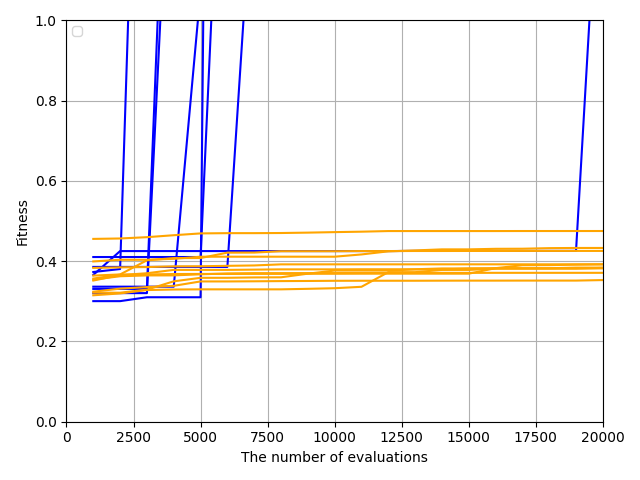
\includegraphics[width=8cm]{exp/linear_regression.png}
  \caption{線形回帰問題における10試行分の既存手法(オレンジ色)と提案手法(青色)の適合度推移. 横軸は評価回数, 縦軸は適合度を意味する. 適合度は初期集団生成後から100回刻みで計測した.}
  \label{fig:exp:result:linear_regression}
\end{figure}

\begin{figure}[H]
  \centering
  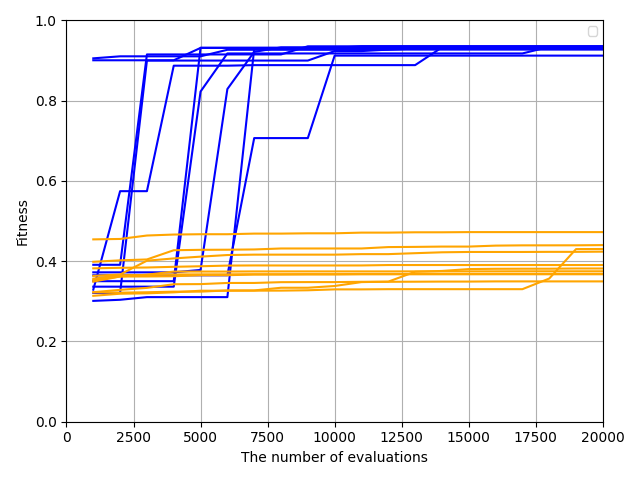
\includegraphics[width=8cm]{exp/noisy_linear_regression.png}
  \caption{$N(0,0.1)$に従うノイズを付与した線形回帰問題における10試行分の既存手法(オレンジ色)と提案手法(青色)の適合度推移. 横軸は評価回数, 縦軸は適合度を意味する. 適合度は初期集団生成後から100回刻みで計測した.}
  \label{fig:exp:result:noisy_linear_regression}
\end{figure}

\begin{figure}[H]
  \centering
  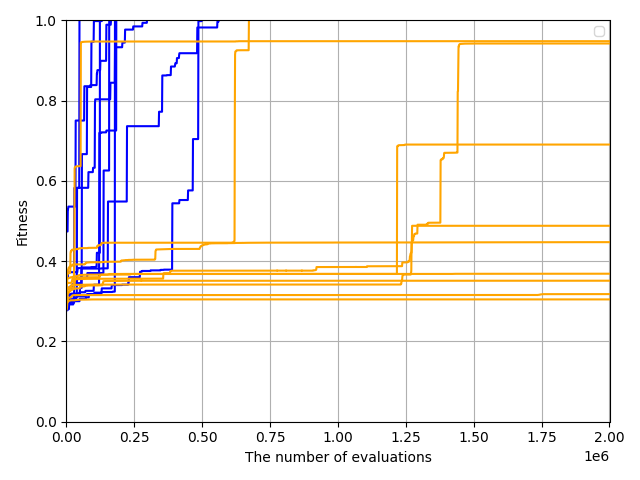
\includegraphics[width=9cm]{exp/affine_regression.png}
  \caption{アフィン回帰問題における10試行分の既存手法(オレンジ色)と提案手法(青色)の適合度推移. 横軸は評価回数, 縦軸は適合度を意味する. 適合度は初期集団生成後から100回刻みで計測した.}
  \label{fig:exp:result:affine_regression}
\end{figure}

\begin{figure}[H]
  \centering
  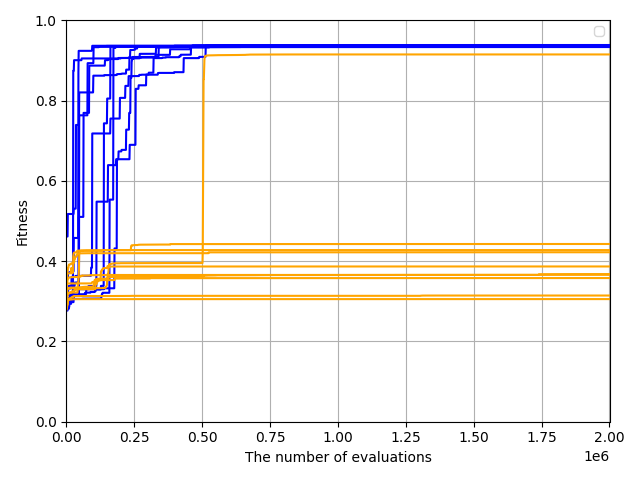
\includegraphics[width=9cm]{exp/noisy_affine_regression.png}
  \caption{$N(0,0.1)$に従うノイズを付与したアフィン回帰問題における10試行分の既存手法(オレンジ色)と提案手法(青色)の適合度推移. 横軸は評価回数, 縦軸は適合度を意味する. 適合度は初期集団生成後から100回刻みで計測した.}
  \label{fig:exp:result:noisy_affine_regression}
\end{figure}

\begin{figure}[H]
  \centering
  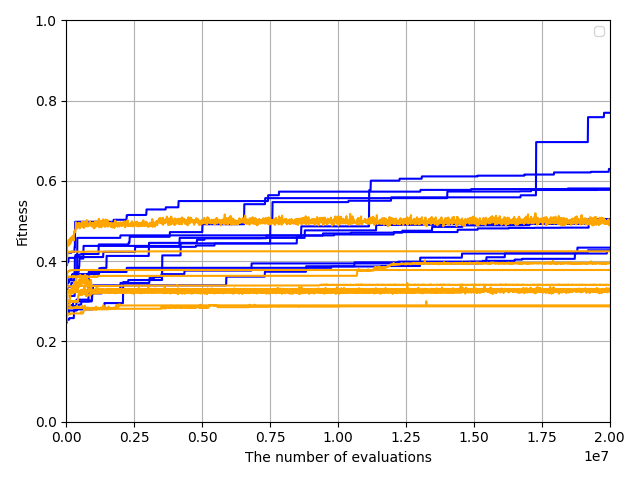
\includegraphics[width=9cm]{exp/two_layers_nn_regression.png}
  \caption{非線形回帰問題における10試行分の既存手法(オレンジ色)と提案手法(青色)の適合度推移. 横軸は評価回数, 縦軸は適合度を意味する. 適合度は初期集団生成後から100回刻みで計測した.}
  \label{fig:exp:result:two_layers_nn_regression}
\end{figure}


\begin{figure}[H]
  \centering
  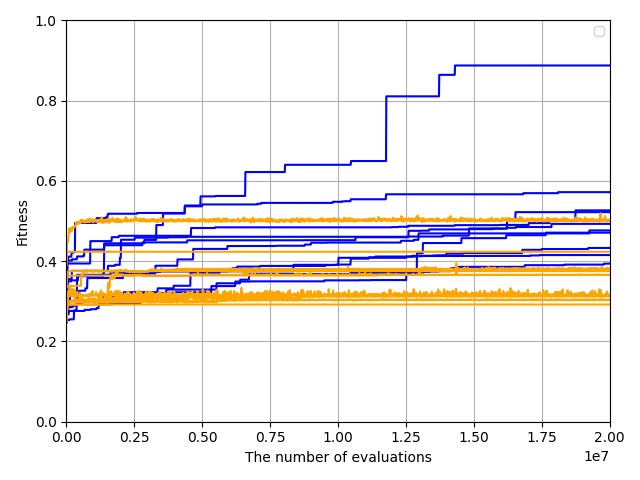
\includegraphics[width=9cm]{exp/noisy_two_layers_nn_regression.png}
  \caption{$N(0,0.1)$に従うノイズを付与した非線形回帰問題における10試行分の既存手法(オレンジ色)と提案手法(青色)の適合度推移. 横軸は評価回数, 縦軸は適合度を意味する. 適合度は初期集団生成後から100回刻みで計測した.}
  \label{fig:exp:result:noisy_two_layers_nn_regression}
\end{figure}

\begin{figure}[H]
  \centering
  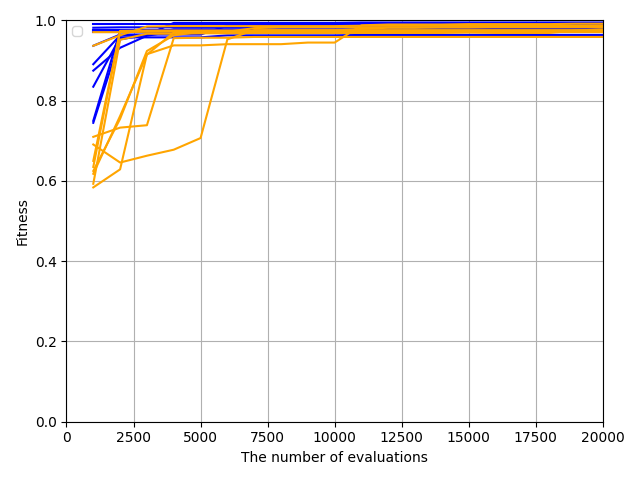
\includegraphics[width=9cm]{exp/linear_classification.png}
  \caption{線形分類問題における10試行分の既存手法(オレンジ色)と提案手法(青色)の適合度推移. 横軸は評価回数, 縦軸は適合度を意味する. 適合度は初期集団生成後から100回刻みで計測した.}
  \label{fig:exp:result:linear_classification}
\end{figure}

\begin{figure}[H]
  \centering
  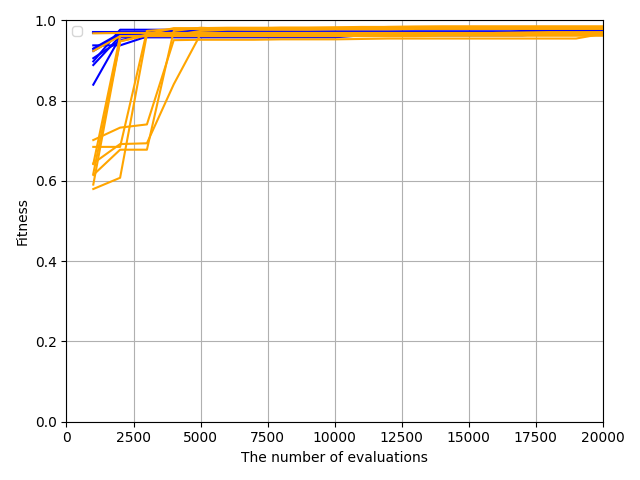
\includegraphics[width=9cm]{exp/noisy_linear_classification.png}
  \caption{$N(0,0.1)$に従うノイズを付与した線形分類問題における10試行分の既存手法(オレンジ色)と提案手法(青色)の適合度推移. 横軸は評価回数, 縦軸は適合度を意味する. 適合度は初期集団生成後から100回刻みで計測した.}
  \label{fig:exp:result:noisy_linear_classification}
\end{figure}

\begin{figure}[H]
  \centering
  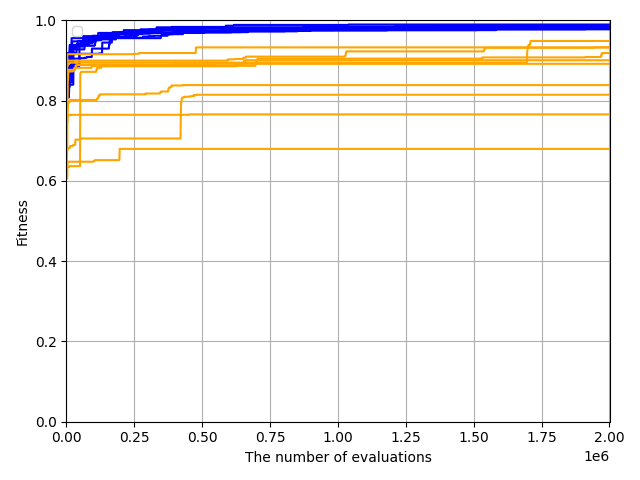
\includegraphics[width=9cm]{exp/affine_classification.png}
  \caption{アフィン分類問題における10試行分の既存手法(オレンジ色)と提案手法(青色)の適合度推移. 横軸は評価回数, 縦軸は適合度を意味する. 適合度は初期集団生成後から100回刻みで計測した.}
  \label{fig:exp:result:affine_classification}
\end{figure}

\begin{figure}[H]
  \centering
  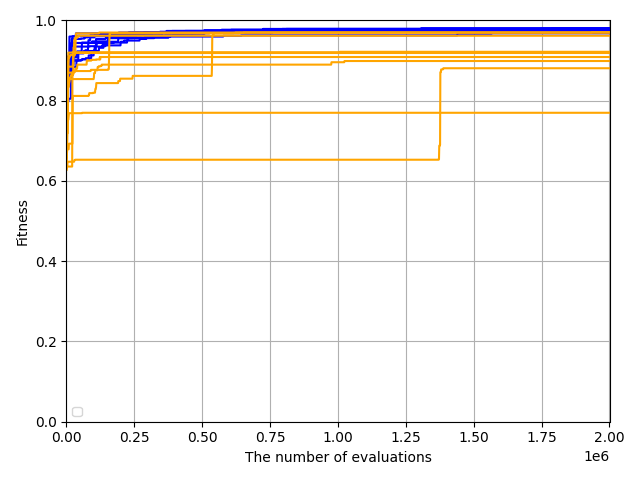
\includegraphics[width=9cm]{exp/noisy_affine_classification.png}
  \caption{$N(0,0.1)$に従うノイズを付与したアフィン分類問題における10試行分の既存手法(オレンジ色)と提案手法(青色)の適合度推移. 横軸は評価回数, 縦軸は適合度を意味する. 適合度は初期集団生成後から100回刻みで計測した.}
  \label{fig:exp:result:noisy_affine_classification}
\end{figure}

\begin{figure}[H]
  \centering
  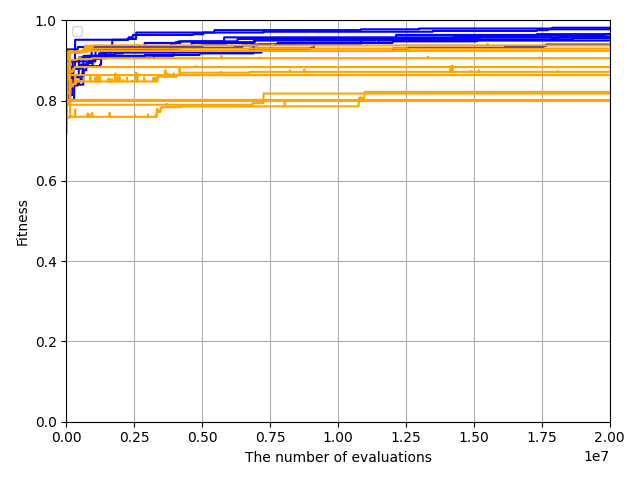
\includegraphics[width=9cm]{exp/two_layers_nn_classification.png}
  \caption{非線形分類問題における10試行分の既存手法(オレンジ色)と提案手法(青色)の適合度推移. 横軸は評価回数, 縦軸は適合度を意味する. 適合度は初期集団生成後から100回刻みで計測した.}
  \label{fig:exp:result:two_layers_nn_classification}
\end{figure}


\begin{figure}[H]
  \centering
  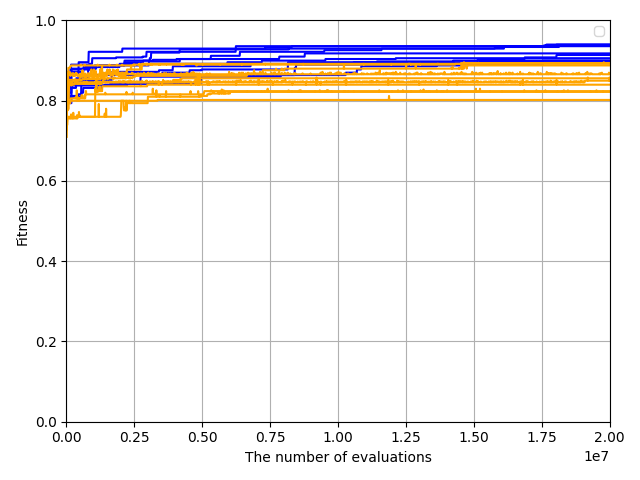
\includegraphics[width=9cm]{exp/noisy_two_layers_nn_classification.png}
  \caption{$N(0,0.1)$に従うノイズを付与した非線形分類問題における10試行分の既存手法(オレンジ色)と提案手法(青色)の適合度推移. 横軸は評価回数, 縦軸は適合度を意味する. 適合度は初期集団生成後から100回刻みで計測した.}
  \label{fig:exp:result:noisy_two_layers_nn_classification}
\end{figure}


\section{探索効率の比較} \label{sec:consideration:efficiency}
提案手法と既存手法の探索効率を比較するために, 第\ref{chap:exp}章の線形回帰の問題設定で, 適合度が1.00になる最適解の発見までにかかる評価回数を比較する実験を行った. 具体的には, 打ち切り評価回数は第\ref{chap:exp}章の実験の1000倍である$2 \times 10^8$回, 打ち切り適合度は0.999を設定して, 最適解が発見されるまでの評価回数を計測した. この実験の結果をTable.\ref{table:exp:result:linear}に示す. この結果より, 提案手法は既存手法のおよそ1/1000の評価回数で最適解の発見に成功していることがわかる.

\begin{table*}[tbp]
  \caption{線形回帰問題において最適解発見までに必要な評価回数の比較. 打ち切り評価回数は$2 \times 10^8$回, 打ち切り適合度は0.999を設定した. 評価回数が書かれていない試行は, 最適解が発見されず打ち切り評価回数に到達した.}
  \label{table:exp:result:linear}
  \centering
  \begin{tabular}{|c|r|r|}
    \hline
    No.  & 既存手法 & 提案手法  \\
    \hline \hline
    1       &  -  & 4,900 \\
    2       &  -  & 19,500  \\
    3       &  -  & 3,400 \\
    4       &  1,423,000  & 2,300 \\
    5       &  12,287,000  & 5,100  \\
    6       &  4,810,000 & 5,400  \\
    7       &  1,885,000 & 3,500  \\
    8       &  6,797,000 & 1,000 \\
    9       &  1,939,000  & 1,000 \\
    10      &  8,658,000  & 6,600 \\
    \hline
    最適解の発見率 & 7/10 & 10/10\\
    平均 & 5,399,857 &  5,270 \\
    標準偏差 & 3,544,279  & 4,828  \\
    \hline
  \end{tabular}
\end{table*}

\begin{figure}[t]
  \begin{lstlisting}[caption=提案手法MGG-AutoML-Zero+VAGによって発見された非線形回帰のアルゴリズム,label=code:found_algorithm,basicstyle=\small\ttfamily]
  def Setup():
    v9[0] = 0.1292114413108869
    v9[1] = -0.2505831388740483
    v9[2] = 0.12620974617641995
    v9[3] = -0.0927704715743739
    v4[0] = 0.25345634793978156
    v4[1] = -0.08198893900983063
    v4[2] = 0.8014245536744797
    v4[3] = 0.010866990780659367
    s3 = 1.4885836334477234
    v1[0] = -0.2070414761633693
    v1[1] = 0.10284085463491824
    v1[2] = 0.2167110168418553
    v1[3] = 0.01683729653416114
    m0[0, 0] = -0.0979146690138854
    m0[0, 1] = 0.04255247850261564
    m0[0, 2] = -0.3568448431607237
    m0[0, 3] = -1.3577788838503895
    m0[1, 0] = 6.035751444417415
    m0[1, 1] = -0.6687873811147038
    m0[1, 2] = -0.16350991278782046
    m0[1, 3] = -0.15973189880280841
    m0[2, 0] = 1.3238446302023488
    m0[2, 1] = -0.2353881355163895
    m0[2, 2] = 2.590326515451852
    m0[2, 3] = 5.842738211926392
    m0[3, 0] = -3.172535391257986
    m0[3, 1] = -2.2259992680585774
    m0[3, 2] = 1.4764090181451432
    m0[3, 3] = 0.314381472387436

  def Predict():
    v8 = dot(m0, v0)
    v10 = maximum(v8, v1)
    s1 = dot(v9, v10)

  def Learn():
    s2 = s0 - s1
    v5 = s2 * v9
    v7 = heaviside(v8, 1.0)
    v6 = s3 * v7
    v3 = v5 * v6
    v2 = s2 * v4
    m1 = outer(v3, v0)
    v1 = v1 + v2
    m0 = m0 + m1
  \end{lstlisting}
  \end{figure}

\section{探索空間の冗長性} \label{sec:consideration:redundancy}

本節では, 既存手法において探索空間がどの程度冗長であるかを定量的に述べる. 具体的には, 第\ref{chap:exp}章の線形回帰問題と同じ探索空間で, 初期個体の生成と同様の方法で100,000個のアルゴリズムを生成した時の非妥当なアルゴリズムの割合を計測した. その結果, 既存手法の探索空間のうち99.9\%以上が非妥当なアルゴリズムであることがわかった.

\section{非妥当な突然変異} \label{sec:consideration:invalid}

本節では, 既存手法における非妥当な突然変異の割合を調査する. この調査は, 第\ref{chap:exp}章の実験のノイズなしの既存手法の線形回帰問題の設定と同様の条件で, 妥当なアルゴリズムを突然変異させた場合に, 非妥当になる割合を計測した. その結果, 既存手法による子個体生成は, 99.6\%以上の割合で, 非妥当な突然変異が発生していることがわかった.

\section{提案手法の各工夫の有効性}

本節では, 我々が導入したアルゴリズムグラフと多様性維持の工夫の有効性を確認するための考察実験について述べる. 考察手法としては, 既存手法と同様のREによる世代交代でアルゴリズムの表現のみをVAGにした手法RE-AutoML-Zero+VAGを用いる. 言い換えれば, RE-AutoML-Zero+VAGには, 提案手法の集団の多様性維持の工夫を除いた手法である. また, 実験は 第\ref{chap:exp}章のノイズなしのアフィン回帰問題設定で行い, 既存手法RE-AutoML-Zero, 考察手法RE-AutoML-Zero+VAG, 提案手法MGG-AutoML-Zero+VAGの最適解発見までの評価回数を比較する.

アフィン回帰問題における実験結果を表\ref{table:exp:result:aggregation:affine_regression}に示す. 表中では, 最適解を発見できなかった試行については評価回数を記載していない. 実験結果から, 既存手法が30試行中わずか1試行でしか最適解を発見できなかったのに対し, 既存手法にVAGを導入した考察手法は全試行において最適解の発見に成功したことがわかる. これは, VAGによって探索空間が効果的に削減され, より効率的な探索が可能になったためと考えられる. 一方で, 考察手法は提案手法と比較すると, 最適解発見までの平均評価回数が多く, その分散も大きくなっている. この結果は, 提案手法で導入した多様性維持の工夫が, 改善の見込みがある有望な個体を集団中に効果的に保持できていることを示唆している.

\begin{table*}[tbp]
  \caption{アフィン回帰問題における考察実験の結果. 既存手法RE-AutoML-Zero, 考察手法RE-AutoML-Zero+VAG, 提案手法MGG-AutoML-Zero+VAGのそれぞれに対して, アフィン回帰問題で最適解を発見するまでにかかった評価回数を示した. 最適解が発見できなかった試行については, 評価回数は書かれていない.}
  \label{table:exp:result:aggregation:affine_regression}
  \centering
  \begin{tabular}{|c|c|c|c|}
    \hline
    No. & 既存手法 & 考察手法 & 提案手法  \\
    \hline \hline
    1       & - & 384,000   & 130,600 \\
    2       & 672,000 & 753,000   & 560,800 \\
    3       & - & 56,000    & 178,600 \\
    4       & - & 72,000    & 157,400 \\
    5       & - & 346,000   &  47,900 \\
    6       & - & 640,000   & 123,100 \\
    7       & - & 10,000    & 163,900 \\
    8       & - & 1,547,000 & 183,500 \\
    9       & - & 818,000   & 498,800 \\
    10      & - & 103,000   & 296,400 \\
    \hline
    最適解の発見率 & 0/10 & 10/10 & 10/10 \\
    平均 &  672,000 & 472,900 & 234,100 \\
    標準偏差& 0 & 435,765 & 152,207 \\
    \hline
  \end{tabular}
\end{table*}

\chapter{結論} \label{chap:conclusion}

\section{本研究のまとめ}

本研究は, Estebanらが提案したAutoML-Zeroにおける探索効率の課題に着目し, AutoML-Zeroの人間の事前知識や介入を最小限にできる利点は残しつつ, 探索効率を改善する手法を提案した. EstebanらのAutoML-Zeroは, 機械学習アルゴリズムの自動探索において画期的な成果を示したものの, 膨大な計算リソースを必要とするという重要な課題が残されていた. 例えば, ReLU関数の再発明に成功した実験では, 1秒間あたり10,000モデルの評価が可能なCPUを搭載したマシンを10,000台使用し, 約5日間という大規模な計算を要した.

本研究では, この探索効率を低下させる要因として, (1)探索空間の冗長性に関する問題, (2)個体の良質な構造を子個体に継承できない問題, (3)集団の多様性維持に関する問題, という3つの課題に着目し, それぞれに対する解決策を提案した.

第一に, 探索空間の冗長性に関する問題に対しては, グラフ構造によるアルゴリズム表現を導入し, 機械学習アルゴリズムとして満たすべき条件を明確に規定した. これにより, 予測ラベルが代入されないアルゴリズムや, 入力ベクトルが予測に利用されていないアルゴリズム, 逐次更新される学習パラメータが存在しないアルゴリズムなど, 機械学習アルゴリズムとして非妥当なものを探索空間から除外することに成功した. その結果, 探索空間を99.9\%以上削減することができた. また, グラフ構造による表現により, 変数名の違いによる冗長性も排除することが可能となった.

第二に, 個体の良質な構造を子個体に継承できない問題に対しては, グラフ構造に基づく新たな突然変異操作を提案した. 既存手法では, 非妥当なアルゴリズムへの突然変異や, 関数全体を破壊的に変更する突然変異が高確率で発生していたが, 提案手法ではグラフ構造の特性を活用することで, 非妥当な突然変異を完全に防止することができた. さらに, 部分グラフの再構築による突然変異を導入することで, 関数内の特定の変数計算に必要な部分命令列のみを局所的に変更することが可能となった.

第三に, 集団の多様性維持に関する問題に対しては, Minimal Generation Gap (MGG)による世代交代モデルを採用し, さらに集団内の同一個体の排除および希少度を考慮した生存選択を導入した. 既存手法では, 世代交代モデルとしてRegularized Evolution (RE)を採用していたことにより, 集団の多様性維持が困難であるという問題が存在した. 加えて, 集団内における個体の重複や希少度が考慮されていなかったため, 同一もしくは類似したアルゴリズムが集団内で過度に増加してしまう傾向があった. そのため, 探索序盤で発見された局所最適なアルゴリズムに早期収束してしまい, 探索効率の低下を招いていた. これに対して提案手法では, MGGによる世代交代モデル, 集団内の同一個体の排除, 希少度を考慮した生存選択を導入することで, 集団の多様性を維持しやすい探索を実現した. これにより, アフィン回帰問題の最適解を発見するまでの評価回数を約1/3にすることができた.

提案手法の有効性を検証するため, ローカルPCという限られた計算リソース環境において, 主要な回帰問題と分類問題を用いた比較実験を実施した. その結果, 非線形回帰問題において, 同一評価回数内で発見されるアルゴリズムの適合度を42\%以上向上することを確認した. 特に, 線形回帰問題においては, 適合度0.999以上のアルゴリズムを発見するまでの評価回数を既存手法の1/1000まで削減することに成功した. これらの結果は, 提案手法が AutoML-Zeroの利点を保持しつつ, 探索効率を大幅に改善できることを示している.

以上の成果は, 機械学習アルゴリズムの自動探索における計算コストの大幅な削減を実現し, より実用的なAutoMLの実現に向けた重要な一歩となることが期待される.

\section{今後の課題}

本研究の今後の課題として, ハイパーパラメータのチューニング, 高度な問題設定による大規模実験の実施, AGの交差の実現が挙げられる. 本節では, それぞれの課題について説明する.

\subsection{ハイパーパラメータのチューニング}

提案手法には多くのハイパーパラメータが存在するが, 現状はそのチューニングができておらず, 一部のパラメータを除いて同一の値を利用し続けている. そのため, 実験に合わせた最適なパラメータの設定は今後の課題である. 突然変異の選択確率などのパラメータは, 探索の状況に合わせて動的に変化させることで, 更なる性能の改善も期待できる. そのため, 探索過程の突然変異やエリート個体を観察した上で, 各ユーザパラメータの推奨値の設定や動的な適応について検討していきたい.

\subsection{高度な問題設定による大規模実験}

本論文の実験では, 限られた命令セットで機械学習の問題設定の中でも比較的簡単な問題を扱って, 探索性能の確認を行った. 実際, 第\ref{chap:exp}章の実験で扱った問題設定は, 4次元の線形回帰問題, アフィン回帰問題, 非線形回帰問題, 線形分類問題, アフィン分類問題, 非線形分類問題であり, これらは基礎的な機械学習のベンチマーク問題として位置づけられる. 非線形の問題であったとしても, 1層のニューラルネットワークで十分高い適合度を達成することができる問題であった. 第\ref{chap:exp}章で述べたように, 命令セットも各問題設定において高い適合度を達成する上で必要な命令セットに限定して実験していた.

しかしながら, 第\ref{sec:consideration:efficiency}節の実験を通して, 線形回帰の問題設定において, 提案手法が既存手法よりも1000倍以上も効率的に探索を行えることが明らかになった. そのため, Estebanらが取り組んでいた全ての命令セットを利用してCIFAR-10やMNISTデータを分類する問題設定に, 限られた計算リソースと時間で挑戦することも現実的になってきたと考えられる. そこで, 大規模実験を通じた提案手法の有効性の検証や, 未知のアルゴリズムの発見に向けた大規模実験をしていきたい.

\subsection{AGの交叉の実現}

現状の提案手法の世代交代においては, 突然変異のみが利用されており交叉が導入されていないため, 複数の親個体の良質な部分構造を継承できる子個体を生成することができない. 一方で, 本論文の貢献として, アルゴリズムをグラフとして構造化することに成功した. そのため, 複数のAGの類似構造や対応関係を取れる仕組みを作ることで, 親個体の2つの性質を持つ子個体を生成する交叉の実現ができる可能性があるため, 交叉の手法について模索していきたい.

\bibliographystyle{jplain}
\bibliography{ref}

\chapter*{謝辞}

本研究を遂行するにあたり, 多大なるご指導とご助言を賜りました小野功教授に深く感謝する. また, ゼミにおいて貴重なご意見や有益なアイデアを頂いた小野功研究室のメンバーにも心より感謝する.

\appendix

\chapter{順序付き有向グラフ} \label{chap:ordered_directed_graph}

\section{はじめに}
本付録では, アルゴリズムグラフの定式化で用いた順序付き有向グラフについて述べる. 順序付き有向グラフとは, 各ノードの子ノード間に順序関係を持つ有向グラフである. 通常の有向グラフがエッジを2つのノードの組$(v_1, v_2)$として表現するのに対し, 順序付き有向グラフではエッジを始点ノード, 自然数で表される順序値, 終点ノードの組$(v_1, n, v_2)$として表現する. この拡張により, 非可換な命令(演算)の入力順序を扱うことが可能となる.

\section{定義}
順序付き有向グラフは, ノードの集合$U$とエッジの集合$E$からなるグラフ$G = (U, E)$である. ここで, $E \subset U \times \mathbb{N} \times U$であり, 各エッジ$e \in E$は, ノード$u_1 \in U$, 順序値$n \in \mathbb{N}$, ノード$u_2 \in U$の順序付きペア$(u_1, n, u_2)$で表現される. また, 同じノードの同じ順序値に複数のエッジを対応させることはできない, 言い換えれば以下の条件を満たす.
\begin{gather*}
\forall u_1, u_2, u_3 \in U,\ \forall n \in \mathbb{N} \\
(u_1, n, u_2) \in E \land (u_1, n, u_3) \in E \Rightarrow u_2 = u_3
\end{gather*}
\noindent
一方で, 順序値が違えば, 同じノード間に複数のエッジを持つことも可能である.

\section{経路と閉路}
順序付き有向グラフにおける経路とは, 以下の条件を満たすエッジの列$(e_1, e_2, \ldots, e_m)$である:
\begin{enumerate}
  \item $e_i = (u_i, n_i, u_{i+1}) \in E$
  \item $i \neq j \Rightarrow u_i \neq u_j$
\end{enumerate}
\noindent
$u_1$, $u_{m+1}$をそれぞれ経路の始点と終点と呼ぶ. また, $u_2, \cdots, u_m$を経由点と呼ぶ. 閉路は, 始点と終点が同じ経路, 言い換えれば$u_1 = u_{m+1}$となる経路である. 閉路を持たない順序付き有向グラフを非巡回順序付き有向グラフと呼ぶ. 非巡回順序付き有向グラフでは, エッジの終点ノードを始点ノードの子ノードとして考えることで, 各ノードに対して, 親ノードの集合, 子ノードの集合, 子孫ノードの集合, 祖先ノードの集合を一意に定義することができる.

AGでは計算の依存関係を表現するため, グラフに閉路が存在してはならないため, AGは非巡回順序付き有向グラフとして定式化した.

\section{トポロジカルソート}
非巡回順序付き有向グラフ$G = (U, E)$のトポロジカルソートとは, 全てのノードを一列に並べた順列$\sigma: \{1,2,\ldots,|U|\} \rightarrow U$であり, 以下の条件を満たす:

\begin{gather*}
\forall (u_1, n, u_2) \in E, \sigma^{-1}(u_1) < \sigma^{-1}(u_2)
\end{gather*}

ここで, $\sigma^{-1}(u)$は順列$\sigma$におけるノード$u$の位置を表す. この条件は, 全てのエッジ$(u_1,n,u_2) \in E$について, $u_1$が$u_2$より前に現れることを意味する. トポロジカルソートは, グラフが非巡回である場合に必ず存在し, 一般に一意ではない. ノードをトポロジカルソートすることで, アルゴリズムグラフにおける命令の実行順序を決定することが可能となる.

具体例として, 以下のグラフを考える:
\begin{itemize}
   \item ノード集合: $U = \{A, B, C\}$
   \item エッジ集合: $E = \{(A,1,B), (A,2,C), (B,1,C)\}$
\end{itemize}
\noindent
このとき, $\sigma: (A,B,C)$はトポロジカルソートとなる.


\section{弱連結性}
順序付き有向グラフが弱連結であるとは, 有向グラフの弱連結性と同様に, 無向グラフとして考えた時の連結性として定義される. 具体的には, 順序付き有向グラフ$G = (U, E)$から, それに対応する無向グラフ$G' = (U, E')$を生成し, $G'$が連結であるとき, $G$は弱連結であるという. ここで, $E' = \{(u_1, u_2)\ |\ (u_1, n, u_2) \in E\}$である. 機械学習アルゴリズムにおいては, 予測ラベルの計算と独立な依存関係を持つ命令は不要であるため, アルゴリズムグラフは弱連結な順序付き有向グラフとして定式化した.

\chapter{命令セット} \label{chap:ops}

本研究のアルゴリズムを構成するための命令セットをTable.\ref{table:instructions}に示す. この命令セットはEstebanらの論文\cite{automl_zero}に使われている命令セットと同様である.

\begin{center}
  {\renewcommand\arraystretch{1.9}
    {\scriptsize
      \begin{longtable}{l|l|lc|lc|l}
        \caption{アルゴリズムの各関数Setup, Predict, Learnを構成する命令の一覧. Estebanらの論文\cite{automl_zero}に示されている命令セットと同様である. }
        \\
        \hline
        \multirow{2}{*}{命令}
             & \multirow{2}{*}{コード例}
             & \multicolumn{2}{c|}{入力}                    & \multicolumn{2}{c|}{出力}
             & \multirow{2}{*}{説明}                                                                                                                                                                          \\
             &                                            & 変数/型                    & 定数              & 変数/型       & 添字                                                                                     \\
        \hline \hline
        \endfirsthead
        \hline
        \multirow{2}{*}{命令ID}
             & \multirow{2}{*}{コード例}
             & \multicolumn{2}{c|}{入力}                    & \multicolumn{2}{c|}{出力}
             & \multirow{2}{*}{説明}                                                                                                                                                                          \\
             &                                            & 変数/型                    & 定数              & 変数/型       & 添字                                                                                     \\
        \hline \hline
        \endhead

        \label{table:instructions}
        OP0  & no\_op                                     & -                       & -               & -          & -     & -                                                                              \\
        OP1  & $s2 = s3 + s0$                             & $a,b$/scalars           & -               & $c$/scalar & -     & $s_c = s_a + s_b$                                                              \\
        OP2  & $s4 = s0 - s1$                             & $a,b$/scalars           & -               & $c$/scalar & -     & $s_c = s_a - s_b$                                                              \\
        OP3  & $s8 = s5 * s5$                             & $a,b$/scalars           & -               & $c$/scalar & -     & $s_c = s_a s_b$                                                                \\
        OP4  & $s7 = s5 / s2$                             & $a,b$/scalars           & -               & $c$/scalar & -     & $s_c = s_a / s_b$                                                              \\
        OP5  & $s8 = \mathrm{abs}(s0)$                    & $a$/scalar              & -               & $b$/scalar & -     & $s_b = |s_a|$                                                                  \\
        OP6  & $s4 = 1/ s8$                               & $a$/scalar              & -               & $b$/scalar & -     & $s_b = 1/s_a$                                                                  \\
        OP7  & $s5 = \mathrm{sin}(s4)$                    & $a$/scalar              & -               & $b$/scalar & -     & $s_b = \mathrm{sin}(s_a)$                                                      \\
        OP8  & $s1 = \mathrm{cos}(s4)$                    & $a$/scalar              & -               & $b$/scalar & -     & $s_b = \mathrm{cos}(s_a)$                                                      \\
        OP9  & $s0 = \mathrm{tan}(s4)$                    & $a$/scalar              & -               & $b$/scalar & -     & $s_b = \mathrm{tan}(s_a)$                                                      \\
        OP10 & $s0 = \mathrm{arcsin}(s4)$                 & $a$/scalar              & -               & $b$/scalar & -     & $s_b = \mathrm{arcsin}(s_a)$                                                   \\
        OP11 & $s2 = \mathrm{arccos}(s0)$                 & $a$/scalar              & -               & $b$/scalar & -     & $s_b = \mathrm{arccos}(s_a)$                                                   \\
        OP12 & $s4 = \mathrm{arctan}(s0)$                 & $a$/scalar              & -               & $b$/scalar & -     & $s_b = \mathrm{arctan}(s_a)$                                                   \\
        OP13 & $s1 = \mathrm{exp}(s2)$                    & $a$/scalar              & -               & $b$/scalar & -     & $s_b = e^{s_a}$                                                                \\
        OP14 & $s0 = \mathrm{log}(s3)$                    & $a$/scalar              & -               & $b$/scalar & -     & $s_b = \log s_a$                                                               \\
        OP15 & $s3 = \mathrm{heaviside}(s0)$              & $a$/scalar              & -               & $b$/scalar & -     & $s_b = \mathbbm{1}_{\mathbb{R}+}(s_a)$                                         \\
        OP16 & $v2 = \mathrm{heaviside}(v2)$              & $a$/vector              & -               & $b$/vector & -     & $\forall i,\bm{v}_b^{(i)} = \mathbbm{1}_{\mathbb{R}+}(\bm{v}_a^{(i)})$         \\
        OP17 & $m7 = \mathrm{heaviside}(m3)$              & $a$/matrix              & -               & $b$/matrix & -     & $\forall i, jM_b^{(i, j)} = \mathbbm{1}_{\mathbb{R}+}(M_a^{(i, j)})$           \\
        OP18 & $v1 = s7 * v1$                             & $a,b$/sc, vec           & -               & $c$/vector & -     & $\bm{v}_c = s_a \bm{v}_b$                                                      \\
        OP19 & $v1 = \mathrm{bcast}(s3)$                  & $a$/scalar              & -               & $b$/vector & -     & $ \forall i,\bm{v}_b^{(i)} = s_a $                                             \\
        OP20 & $v5 = 1/v7$                                & $a$/vector              & -               & $b$/vector & -     & $ \forall i,\bm{v}_b^{(i)} = 1/s_a^{(i)} $                                     \\
        OP21 & $s0 = \mathrm{norm}(v3)$                   & $a$/scalar              & -               & $b$/vector & -     & $s_b = \left\| \bm{v}_a \right\|$                                              \\
        OP22 & $v3 = \mathrm{abs}(v3)$                    & $a$/vector              & -               & $b$/vector & -     & $\forall i,\bm{v}_b^{(i)} = \left| \bm{v}_a^{(i)} \right|$                     \\

        OP23 & $v5 = v0 + v9$                             & $a,b$/vectors           & -               & $c$/scalar & -     & $\bm{v}_c = \bm{v}_a + \bm{v}_b$                                               \\
        OP24 & $v1 = v0 - v9$                             & $a,b$/vectors           & -               & $c$/scalar & -     & $\bm{v}_c = \bm{v}_a - \bm{v}_b$                                               \\
        OP25 & $v8 = v0 * v9$                             & $a,b$/vectors           & -               & $c$/scalar & -     & $\forall i,\bm{v}_c^{(i)} = \bm{v}_a^{(i)} \bm{v}_b^{(i)}$                     \\
        OP26 & $v9 = v8 / v2$                             & $a,b$/vectors           & -               & $c$/scalar & -     & $\forall i,\bm{v}_c^{(i)} = \bm{v}_a^{(i)} / \bm{v}_b^{(i)}$                   \\
        OP27 & $s6 = \mathrm{dot}(v1, v5)$                & $a,b$/vectors           & -               & $c$/scalar & -     & $s_c = \bm{v}_a^T \bm{v}_b$                                                    \\
        OP28 & $m1 = \mathrm{outer}(v6, v5)$              & $a,b$/vectors           & -               & $c$/matrix & -     & $M_c = \bm{v}_a\bm{v}_b^T$                                                     \\
        OP29 & $m1 = a4 * m2$                             & $a,b$/sc/mat            & -               & $c$/matrix & -     & $M_c = s_a M_b$                                                                \\
        OP30 & $m3 = 1/m0$                                & $a$/matrix              & -               & $b$/matrix & -     & $ \forall i,j, M_b^{(i,j)} = 1/M_a^{(i, j)} $                                  \\
        OP31 & $v6 = \mathrm{dot}(m1, v0)$                & $a,b$/mat/vec           & -               & $c$/vector & -     & $\bm{v}_c = M_a \bm{v}_b$                                                      \\
        OP32 & $m2 = \mathrm{bcast}(v0, \mathrm{axis}=0)$ & $a$/vector              & -               & $b$/matrix & -     & $\forall i,j,M_b^{(i,j)}= \bm{v}_a^{(i)}$                                      \\
        OP33 & $m2 = \mathrm{bcast}(v0, \mathrm{axis}=1)$ & $a$/vector              & -               & $b$/matrix & -     & $\forall i,j,M_b^{(j,i)}= \bm{v}_a^{(i)}$                                      \\
        OP34 & $s2 = \mathrm{norm}(m1)$                   & $a$/matrix              & -               & $b$/scalar & -     & $s_b = \left\| \bm{v}_a \right\|$                                              \\
        OP35 & $v4 = \mathrm{norm}(m7, \mathrm{axis}=0)$  & $a$/matrix              & -               & $b$/vector & -     & $\forall i, \bm{v}_b^{(i)} = \left\| M_a^{(i, \cdot)} \right\|$                \\
        OP36 & $v4 = \mathrm{norm}(m7, \mathrm{axis}=1)$  & $a$/matrix              & -               & $b$/vector & -     & $\forall i, \bm{v}_b^{(i)} = \left\| M_a^{(\cdot, i)} \right\|$                \\
        OP37 & $m9 = \mathrm{transpose}(m3)$              & $a$/matrix              & -               & $b$/matrix & -     & $M_b = M_a^T$                                                                  \\
        OP38 & $m1 = \mathrm{abs}(m8)$                    & $a$/matrix              & -               & $b$/matrix & -     & $ \forall i,j, M_b^{(i,j)} = \left|M_a^{(i, j)}\right| $                       \\
        OP39 & $m2 = m2 + m0$                             & $a,b$/matrixes          & -               & $c$/matrix & -     & $M_c = M_a + M_b$                                                              \\
        OP40 & $m2 = m3 - m1$                             & $a,b$/matrixes          & -               & $c$/matrix & -     & $M_c = M_a - M_b$                                                              \\
        OP41 & $m3 = m2 * m3$                             & $a,b$/matrixes          & -               & $c$/matrix & -     & $\forall i,j, M_c^{(i,j)} = M_a^{(i,j)} M_b^{(i,j)}$                           \\
        OP42 & $m4 = m2 / m4$                             & $a,b$/matrixes          & -               & $c$/matrix & -     & $\forall i,j, M_c^{(i,j)} = M_a^{(i,j)} / M_b^{(i,j)}$                         \\
        OP43 & $m5 = \mathrm{matmul}(m5, m7)$             & $a,b$/matrixes          & -               & $c$/matrix & -     & $M_c = M_a M_b$                                                                \\
        OP44 & $s1 = \mathrm{minimun}(s2, s3)$            & $a,b$/scalars           & -               & $c$/scalar & -     & $s_c = \min{(s_a,s_b)}$                                                        \\
        OP45 & $v4 = \mathrm{minimun}(v3, v9)$            & $a,b$/vectors           & -               & $c$/vector & -     & $\forall i,\bm{v}_c^{(i)} = \min{\left(\bm{v}_a^{(i)},\bm{v}_b^{(i)}\right)}$  \\
        OP46 & $m5 = \mathrm{minimun}(m5, m7)$            & $a,b$/matrixes          & -               & $c$/matrix & -     & $\forall i,j,M_c^{(i,j)} = \min{\left(M_a^{(i,j)}, M_b^{(i,j)}\right)}$        \\
        OP47 & $s8 = \mathrm{maximum}(s3, s0)$            & $a,b$/scalars           & -               & $c$/scalar & -     & $s_c = \max{(s_a,s_b)}$                                                        \\
        OP48 & $v7 = \mathrm{maximum}(v3, v6)$            & $a,b$/vectors           & -               & $c$/vector & -     & $\forall i, \bm{v}_c^{(i)} = \max{\left(\bm{v}_a^{(i)},\bm{v}_b^{(i)}\right)}$ \\
        OP49 & $m7 = \mathrm{maximum}(m1, m0)$            & $a,b$/matrixes          & -               & $c$/matrix & -     & $\forall i,j, M_c^{(i,j)} = \max{\left(M_a^{(i,j)}, M_b^{(i,j)}\right)}$       \\
        OP50 & $s2 = \mathrm{mean}(v2)$                   & $a$/vector              & -               & $b$/scalar & -     & $s_b = \mathrm{mean}\left(\bm{v}_a\right)$                                     \\
        OP51 & $s2 = \mathrm{mean}(m8)$                   & $a$/matrix              & -               & $b$/scalar & -     & $s_b = \mathrm{mean}\left(M_a\right)$                                          \\
        OP52 & $v1 = \mathrm{mean}(m2, \mathrm{axis}=0)$  & $a$/matrix              & -               & $b$/vector & -     & $\forall i,\bm{v}_b^{(i)} = \mathrm{mean}\left(M_a^{(i,\cdot)}\right)$         \\
        OP53 & $v3 = \mathrm{stdev}(m2, \mathrm{axis}=0)$ & $a$/matrix              & -               & $b$/vector & -     & $\forall i,\bm{v}_b^{(i)} = \mathrm{stdev}\left(M_a^{(i,\cdot)}\right)$        \\
        OP54 & $s3 = \mathrm{stdev}(v3)$                  & $a$/vector              & -               & $b$/scalar & -     & $s_b = \mathrm{stdev}\left(\bm{v}_a\right)$                                    \\
        OP55 & $s4 = \mathrm{stdev}(m0)$                  & $a$/matrix              & -               & $b$/scalar & -     & $s_b = \mathrm{stdev}\left(M_a\right)$                                         \\
        OP56 & s2 = 0.7                                   & -                       & $ \gamma $      & $a$/scalar & -     & $s_a = \gamma $                                                                \\
        OP57 & v3[5] = -2.4                               & -                       & $\gamma$        & $a$/vector & $i$   & $\bm{v}_a^{(i)} = \gamma $                                                     \\
        OP58 & m2[5,1] = -0.03                            & -                       & $\gamma$        & $a$/matrix & $i,j$ & $M^{(i,j)}= \gamma$                                                            \\
        OP59 & $s4 = \mathrm{uniform}(-1,1)$              & -                       & $\alpha, \beta$ & $a$/scalar & -     & $s_a = \mathcal{U}(\alpha, \beta)$                                             \\
        OP60 & $v1 = \mathrm{uniform}(0.4,0.8)$           & -                       & $\alpha, \beta$ & $a$/vector & -     & $\forall i, \bm{v}_a^{(i)} = \mathcal{U}(\alpha, \beta)$                       \\
        OP61 & $m0 = \mathrm{uniform}(-0.5,0.6)$          & -                       & $\alpha, \beta$ & $a$/vector & -     & $\forall i, j, M_a^{(i, j)} = \mathcal{U}(\alpha, \beta)$                      \\
        OP62 & $s4 = \mathrm{gaussian}(0.1,0.7)$          & -                       & $\mu, \sigma$   & $a$/scalar & -     & $s_a = \mathcal{N}(\mu, \sigma)$                                               \\
        OP63 & $v8 = \mathrm{gaussian}(0.4,1)$            & -                       & $\mu, \sigma$   & $a$/vector & -     & $\forall i, \bm{v}_a^{(i)} = \mathcal{N}(\mu, \sigma)$                         \\
        OP64 & $m2 = \mathrm{gaussian}(-2,1.3)$           & -                       & $\mu, \sigma$   & $a$/vector & -     & $\forall i, j, M_a^{(i, j)} = \mathcal{N}(\mu, \sigma)$                        \\
        \hline
      \end{longtable}}}
\end{center}

\end{document}
